\documentclass[a4paper,10pt,final]{ThesisStyle}
%\documentclass[a4paper,11pt,draft]{ThesisStyle}

\usepackage{amsmath,amssymb}             % AMS Math
% \usepackage[french]{babel}
%\usepackage[latin1]{inputenc}
\usepackage[T1]{fontenc}
%\usepackage[left=1.5in,right=1.3in,top=1.1in,bottom=1.1in,includefoot,includehead,headheight=13.6pt]{geometry}
\usepackage[left=1.5in,right=1.5in,top=1.25in,bottom=1.25in,headheight=13.6pt]{geometry}
\renewcommand{\baselinestretch}{1.05}

% Table of contents for each chapter

\usepackage[nottoc, notlof, notlot]{tocbibind}
\usepackage{caption}
\usepackage{minitoc}
\setcounter{minitocdepth}{2}
\mtcindent=15pt
% Use \minitoc where to put a table of contents

\usepackage{aecompl}

% Glossary / list of abbreviations

\usepackage[intoc]{nomencl}
\renewcommand{\nomname}{List of Abbreviations}

\makenomenclature

% My pdf code

\usepackage{ifpdf}

\ifpdf
  \usepackage[pdftex]{graphicx}
  \DeclareGraphicsExtensions{.jpg}
  \usepackage[a4paper,pagebackref,hyperindex=true]{hyperref}
\else
  \usepackage{graphicx}
  \DeclareGraphicsExtensions{.ps,.eps}
  \usepackage[a4paper,dvipdfm,pagebackref,hyperindex=true]{hyperref}
\fi

\graphicspath{{.}{images/}}

% nicer backref links
\renewcommand*{\backref}[1]{}
\renewcommand*{\backrefalt}[4]{%
\ifcase #1 %
(Not cited.)%
\or
(Cited on page~#2.)%
\else
(Cited on pages~#2.)%
\fi}
\renewcommand*{\backrefsep}{, }
\renewcommand*{\backreftwosep}{ and~}
\renewcommand*{\backreflastsep}{ and~}

% Links in pdf
\usepackage{color}
\definecolor{linkcol}{rgb}{0.1,0.3,0.7} 
\definecolor{citecol}{rgb}{0.5,0.1,0.1} 

% Change this to change the informations included in the pdf file

% See hyperref documentation for information on those parameters

\hypersetup
{
bookmarksopen=true,
pdftitle="Computational Audiovisual Scene Synthesis",
pdfauthor="Parag Mital", 
pdfsubject="encoding decoding perception modeling collage arts", %subject of the document
%pdftoolbar=false, % toolbar hidden
pdfmenubar=true, %menubar shown
pdfhighlight=/O, %effect of clicking on a link
colorlinks=true, %couleurs sur les liens hypertextes
pdfpagemode=None, %aucun mode de page
pdfpagelayout=SinglePage, %ouverture en simple page
pdffitwindow=true, %pages ouvertes entierement dans toute la fenetre
linkcolor=linkcol, %couleur des liens hypertextes internes
citecolor=citecol, %couleur des liens pour les citations
urlcolor=linkcol %couleur des liens pour les url
}

% definitions.
% -------------------

\setcounter{secnumdepth}{3}
\setcounter{tocdepth}{2}

% Some useful commands and shortcut for maths:  partial derivative and stuff

\newcommand{\pd}[2]{\frac{\partial #1}{\partial #2}}
\def\abs{\operatorname{abs}}
\def\argmax{\operatornamewithlimits{arg\,max}}
\def\argmin{\operatornamewithlimits{arg\,min}}
\def\diag{\operatorname{Diag}}
\newcommand{\eqRef}[1]{(\ref{#1})}

\usepackage{rotating}                    % Sideways of figures & tables
%\usepackage{bibunits}
%\usepackage[sectionbib]{chapterbib}          % Cross-reference package (Natural BiB)
%\usepackage{natbib}                  % Put References at the end of each chapter
                                         % Do not put 'sectionbib' option here.
                                         % Sectionbib option in 'natbib' will do.
\usepackage{fancyhdr}                    % Fancy Header and Footer

% \usepackage{txfonts}                     % Public Times New Roman text & math font
  
%%% Fancy Header %%%%%%%%%%%%%%%%%%%%%%%%%%%%%%%%%%%%%%%%%%%%%%%%%%%%%%%%%%%%%%%%%%
% Fancy Header Style Options

\pagestyle{fancy}                       % Sets fancy header and footer
\fancyfoot{}                            % Delete current footer settings

%\renewcommand{\chaptermark}[1]{         % Lower Case Chapter marker style
%  \markboth{\chaptername\ \thechapter.\ #1}}{}} %

%\renewcommand{\sectionmark}[1]{         % Lower case Section marker style
%  \markright{\thesection.\ #1}}         %

\fancyheadoffset[LE, RE, LO, RO]{1.7cm}
\fancyfootoffset[LE, RE, LO, RO]{1.7cm}
\fancyhead[LE]{\makebox[1.7cm][l]{\bfseries\thepage}}    % Page number (boldface) in left on even
\fancyhead[RO]{\makebox[1.7cm][r]{\bfseries\thepage}}    % Page number (boldface) in left on even
% pages and right on odd pages
%\fancyhead[RE]{\bfseries\nouppercase{\leftmark}}      % Chapter in the right on even pages
%\fancyhead[LO]{\bfseries\nouppercase{\rightmark}}     % Section in the left on odd pages
%\fancyfoot[RE,LO]{\bfseries{Parag K. Mital | Computational Audiovisual Scene Synthesis}}
\fancyhead[RE]{\makebox[1.7cm][r]{\bfseries\nouppercase{\rightmark}}}     % Section in the left on odd pages
\fancyhead[LO]{\makebox[1.7cm][l]{\bfseries\nouppercase{\rightmark}}}     % Section in the left on odd pages
\fancyfoot[LO]{\makebox[1.7cm][l]{\bfseries\nouppercase{\leftmark}}}
\fancyfoot[RE]{\makebox[1.7cm][r]{\bfseries\nouppercase{\leftmark}}}
\fancyfoot[LE]{\makebox[1.7cm][l]{\bfseries\thepage}}    % Page number (boldface) in left on even
\fancyfoot[RO]{\makebox[1.7cm][r]{\bfseries\thepage}}    % Page number (boldface) in left on even

\let\headruleORIG\headrule
\renewcommand{\headrule}{\color{black} \headruleORIG}
\renewcommand{\headrulewidth}{1.0pt}
\let\footruleORIG\footrule
\renewcommand{\footrule}{\color{black} \footruleORIG}
\renewcommand{\footrulewidth}{1.0pt}

\usepackage{colortbl}
\arrayrulecolor{black}

\fancypagestyle{plain}{
  \fancyhead{}
  \fancyfoot{}
  \renewcommand{\headrulewidth}{0pt}
\fancyfoot[LE]{\makebox[1.7cm][l]{\bfseries\thepage}}    % Page number (boldface) in left on even
\fancyfoot[RO]{\makebox[1.7cm][r]{\bfseries\thepage}}    % Page number (boldface) in left on even
}

\usepackage{algorithm}
\usepackage[noend]{algorithmic}

%%% Clear Header %%%%%%%%%%%%%%%%%%%%%%%%%%%%%%%%%%%%%%%%%%%%%%%%%%%%%%%%%%%%%%%%%%
% Clear Header Style on the Last Empty Odd pages
\makeatletter

\def\cleardoublepage{\clearpage\if@twoside \ifodd\c@page\else%
  \hbox{}%
  \thispagestyle{empty}%              % Empty header styles
  \newpage%
  \if@twocolumn\hbox{}\newpage\fi\fi\fi}

\makeatother
 
%%%%%%%%%%%%%%%%%%%%%%%%%%%%%%%%%%%%%%%%%%%%%%%%%%%%%%%%%%%%%%%%%%%%%%%%%%%%%%% 
% Prints your review date and 'Draft Version' (From Josullvn, CS, CMU)
\newcommand{\reviewtimetoday}[2]{\special{!userdict begin
    /bop-hook{gsave 20 710 translate 45 rotate 0.8 setgray
      /Times-Roman findfont 12 scalefont setfont 0 0   moveto (#1) show
      0 -12 moveto (#2) show grestore}def end}}
% You can turn on or off this option.
% \reviewtimetoday{\today}{Draft Version}
%%%%%%%%%%%%%%%%%%%%%%%%%%%%%%%%%%%%%%%%%%%%%%%%%%%%%%%%%%%%%%%%%%%%%%%%%%%%%%% 

\newenvironment{maxime}[1]
{
\vspace*{0cm}
\hfill
\begin{minipage}{0.5\textwidth}%
%\rule[0.5ex]{\textwidth}{0.1mm}\\%
\hrulefill $\:$ {\bf #1}\\
%\vspace*{-0.25cm}
\it 
}%
{%

\hrulefill
\vspace*{0.5cm}%
\end{minipage}
}

\let\minitocORIG\minitoc
\renewcommand{\minitoc}{\minitocORIG \vspace{1.5em}}

\usepackage{multirow}
\usepackage{slashbox}

\newenvironment{bulletList}%
{ \begin{list}%
	{$\bullet$}%
	{\setlength{\labelwidth}{25pt}%
	 \setlength{\leftmargin}{30pt}%
	 \setlength{\itemsep}{\parsep}}}%
{ \end{list} }

\newtheorem{definition}{D�finition}
\renewcommand{\epsilon}{\varepsilon}

% centered page environment

\newenvironment{vcenterpage}
{\newpage\vspace*{\fill}\thispagestyle{empty}\renewcommand{\headrulewidth}{0pt}}
{\vspace*{\fill}}


\usepackage{wrapfig}
\usepackage{hyperref}
\usepackage{fixltx2e}
\usepackage{color}
\usepackage{listings}
\usepackage{afterpage}
\usepackage{algorithm}
\usepackage{algorithmic}
\usepackage{float}
\usepackage{hyperref}
\usepackage{natbib}
%\usepackage[authoryear,round]{natbib}
\usepackage{epigraph}
\usepackage{graphicx}
\usepackage{subcaption}
\usepackage{setspace}
\usepackage{framed}
\usepackage{lipsum}
\usepackage{enumitem}

\setlist{labelwidth=\widthof{0.},leftmargin={\labelwidth+\labelsep+10pt},rightmargin=\leftmargin}

%% Stuff for making gray background in different environments 
\definecolor{light-gray}{gray}{0.95}
\renewenvironment{leftbar}[1][\hsize]
{%
    \def\FrameCommand
    {%
        {\hspace{-3pt}\color{black}\vrule width 3pt}%
        \hspace{0pt}%must no space.
        \fboxsep=1.0pt\colorbox{light-gray}%
    }%
    \MakeFramed{\hsize#1\advance\hsize-\width\FrameRestore}%
}%
{\endMakeFramed}%
\newenvironment{quotationb}%
{\begin{samepage}\begin{leftbar}\begin{quotation}}%
{\end{quotation}\end{leftbar}\end{samepage}}%
\newenvironment{verseb}%
{\begin{samepage}\begin{leftbar}\begin{verse}}%
{\end{verse}\end{leftbar}\end{samepage}}%
\newenvironment{equationb}%
{\begin{leftbar}\begin{equation}}%
{\end{equation}\end{leftbar}}%
\newenvironment{eqnarrayb}%
{\begin{leftbar}\begin{eqnarray}}%
{\end{eqnarray}\end{leftbar}}%
\newenvironment{enumerateb}%
{\begin{samepage}\begin{leftbar}\begin{enumerate}\vspace{5pt}}%
{\end{enumerate}\end{leftbar}\end{samepage}}%
\newenvironment{itemizeb}%
{\begin{samepage}\begin{leftbar}\begin{itemize}}%
{\end{itemize}\end{leftbar}\end{samepage}}%

%\usepackage[raggedright]{titlesec}
%\newlength\mylen
%\setlength\mylen{\dimexpr\oddsidemargin+\hoffset\relax}
%\titleformat{\section}
%  {\normalfont\Large\bfseries}
%  {\llap{\hspace*{-\mylen}\thesection\hfill}}{0em}{}
%  [{\makebox[\linewidth][l]{%
%      \hspace*{-\mylen}\rule{0.6\mylen}{1pt}}}]
%    \hspace*{-\mylen}\rule{\dimexpr\textwidth+\mylen\relax}{1pt}}}]
% More space between paragraphs
 \setlength{\parskip}{6pt}
\allowdisplaybreaks
\raggedbottom

% Remove line in epigraphs
\setlength{\epigraphwidth}{0.6\textwidth}
\setlength{\epigraphrule}{0pt}
\setcounter{tocdepth}{3}
\setcounter{minitocdepth}{3}
\newcommand{\suchthat}{\;\ifnum\currentgrouptype=16 \middle\fi|\;}

% FLOAT
\floatstyle{ruled}
\newfloat{program}{thp}{lop}
\floatname{program}{Program}
\newenvironment{abstract}{\rightskip1in\itshape}{}

\usepackage[yyyymmdd,hhmmss]{datetime}
\usepackage{setspace}
\onehalfspacing
\usepackage{soul}
%\newcommand{\hl}[1]{\colorbox{yellow}{#1}}
\usepackage[strict]{changepage}

%Place line under Figure caption
\DeclareCaptionFormat{myformat}{#1#2#3\hrulefill}
%\captionsetup[figure]{format=myformat}

%%% Define a new caption separator
\definecolor{mybluecolor}{rgb}{.204,.486,.741}
\DeclareCaptionLabelSeparator*{newlinerule}{\par\kern2pt\hrule\kern1pt}
% set up labelformat and labelsep for figure
%\captionsetup[figure]{labelformat=parens, labelsep=newline}
% set up labelformat and labelsep for subfigure

\captionsetup[figure]{%
%  figurename=FIGURE,
%  font=small,
%  format=plain,
  labelformat=simple,
%  labelsep=newlinerule,
  singlelinecheck=off,
  format=myformat
  %labelfont={color=mybluecolor,bf},
}
\captionsetup[subfigure]{singlelinecheck=on,format=plain}
\usepackage{flafter}
\usepackage[bottom]{footmisc}
%\usepackage{helvet}
%\renewcommand{\familydefault}{\sfdefault}

%%%%%%%%%%%%%%%%%%%%%%%%%%%%%%%%%%%%%%%%%%%%%%%%%%%
%%%%%%%%%%%%%%%%%%%%%%%%%%%%%%%%%%%%%%%%%%%%%%%%%%%
%%%%%%%%%%%%%%%%%%%%%%%%%%%%%%%%%%%%%%%%%%%%%%%%%%%
%%%%%%%%%%%%%%%%%%%%%%%%%%%%%%%%%%%%%%%%%%%%%%%%%%%
%%%%%%%%%%%%%%%%%%%%%%%%%%%%%%%%%%%%%%%%%%%%%%%%%%%
%%%%%%%%%%%%%%%%%%%%%%%%%%%%%%%%%%%%%%%%%%%%%%%%%%%
%%%%%%%%%%%%%%%%%%%%%%%%%%%%%%%%%%%%%%%%%%%%%%%%%%%



%%%%%%%%%%%%%%%%%%%%%%%%%%%%%%%%%%%%%%%%%%%%%%%%%%%
%%%%%%%%%%%%%%%%%%%%%%%%%%%%%%%%%%%%%%%%%%%%%%%%%%%
%%%%%%%%%%%%%%%%%%%%%%%%%%%%%%%%%%%%%%%%%%%%%%%%%%%
%%%%%%%%%%%%%%%%%%%%%%%%%%%%%%%%%%%%%%%%%%%%%%%%%%%
%%%%%%%%%%%%%%%%%%%%%%%%%%%%%%%%%%%%%%%%%%%%%%%%%%%
%%%%%%%%%%%%%%%%%%%%%%%%%%%%%%%%%%%%%%%%%%%%%%%%%%%
%%%%%%%%%%%%%%%%%%%%%%%%%%%%%%%%%%%%%%%%%%%%%%%%%%%


\begin{document}

\begin{titlepage}
\begin{center}
\begin{figure} 
\centering

\includegraphics[width=0.5\textwidth]{images/goldsmiths.png}
\end{figure}
%\noindent \Large Goldsmiths, University of London \\
%\noindent \Large \textbf{Specialty : \textsc{Arts and Computational Technologies}}\\
\vspace{1.2cm}
%\noindent \large {Defended by\\}
\noindent {\Huge \textbf{Audiovisual Scene Synthesis}} \\
\vspace{1.2cm}
\noindent \LARGE Parag Kumar \textsc{Mital} \\
\vspace{0.2cm}
\noindent \Large Member of the \textsc{Embodied Audio-Visual Interaction} Lab\\
\vspace{1.2cm}
\noindent \large {thesis submitted in partial fulfillment for the title of} \\
\vspace{0.2cm}
\noindent \LARGE \textbf{PhD of Arts and Computational Technologies} \\
\vspace{0.2cm}
\noindent {\large \textbf{from GOLDSMITHS - UNIVERSITY OF LONDON}} \\
\vspace{1.2cm}
\begin{center}
\noindent \large \textbf{Advisors}
\vspace{0.25cm}
\begin{tabular}{lcl}
Michael \textsc{Grierson} & - & Goldsmiths, University of London\\
Timothy \textsc{Smith}  & - & Birkbeck, University of London\\
\end{tabular}
\end{center}
\vspace{0.5cm}
\end{center}
%\noindent \large \textbf{Jury :} \\
\begin{center}
\noindent \large \textbf{Examiners}
\vspace*{0.25cm}
\begin{tabular}{lcl}
John \textsc{Lee}		& - & University of Edinburgh\\
Matthew \textsc{Fuller}		& - & Goldsmiths, University of London\\
%      \textit{Advisor :}	& Gr�goire \textsc{Malandain}		& - & INRIA (Asclepios)\\
%      \textit{President :}	& Nicholas \textsc{Ayache}		& - & INRIA (Asclepios)\\
%      \textit{Examinators :}   & Pierre-Yves \textsc{Bondiau}          & - & Centre Antoine Lacassagne (Nice)\\
%      				& Guido \textsc{Gerig}			& - & University of North Carolina\\
%      				& Vincent \textsc{Gr�goire}		& - & Universit� Catholique de Louvain\\
%      \textit{Invited :}		& Hanna \textsc{Kafrouni}		& - & DOSISoft S.A.
\end{tabular}
\vspace*{0.4cm}
\end{center}
\end{titlepage}
\sloppy

\titlepage

\dominitoc
\pagenumbering{roman}
 \cleardoublepage
 
 
%%%%%%%%%%%%%%%%%%%%%%%%%%%%%%%%%%%%%%%%%%%%%%%%%%%
%%%%%%%%%%%%%%%%%%%%%%%%%%%%%%%%%%%%%%%%%%%%%%%%%%%
%%%%%%%%%%%%%%%%%%%%%%%%%%%%%%%%%%%%%%%%%%%%%%%%%%%
%%%%%%%%%%%%%%%%%%%%%%%%%%%%%%%%%%%%%%%%%%%%%%%%%%%
%%%%%%%%%%%%%%%%%%%%%%%%%%%%%%%%%%%%%%%%%%%%%%%%%%%
%%%%%%%%%%%%%%%%%%%%%%%%%%%%%%%%%%%%%%%%%%%%%%%%%%%
%%%%%%%%%%%%%%%%%%%%%%%%%%%%%%%%%%%%%%%%%%%%%%%%%%%



%%%%%%%%%%%%%%%%%%%%%%%%%%%%%%%%%%%%%%%%%%%%%%%%%%%
%%%%%%%%%%%%%%%%%%%%%%%%%%%%%%%%%%%%%%%%%%%%%%%%%%%
%%%%%%%%%%%%%%%%%%%%%%%%%%%%%%%%%%%%%%%%%%%%%%%%%%%
%%%%%%%%%%%%%%%%%%%%%%%%%%%%%%%%%%%%%%%%%%%%%%%%%%%
%%%%%%%%%%%%%%%%%%%%%%%%%%%%%%%%%%%%%%%%%%%%%%%%%%%
%%%%%%%%%%%%%%%%%%%%%%%%%%%%%%%%%%%%%%%%%%%%%%%%%%%
%%%%%%%%%%%%%%%%%%%%%%%%%%%%%%%%%%%%%%%%%%%%%%%%%%%


\section*{Acknowledgments}
\lipsum[1-3]



%%%%%%%%%%%%%%%%%%%%%%%%%%%%%%%%%%%%%%%%%%%%%%%%%%%
%%%%%%%%%%%%%%%%%%%%%%%%%%%%%%%%%%%%%%%%%%%%%%%%%%%
%%%%%%%%%%%%%%%%%%%%%%%%%%%%%%%%%%%%%%%%%%%%%%%%%%%
%%%%%%%%%%%%%%%%%%%%%%%%%%%%%%%%%%%%%%%%%%%%%%%%%%%
%%%%%%%%%%%%%%%%%%%%%%%%%%%%%%%%%%%%%%%%%%%%%%%%%%%
%%%%%%%%%%%%%%%%%%%%%%%%%%%%%%%%%%%%%%%%%%%%%%%%%%%
%%%%%%%%%%%%%%%%%%%%%%%%%%%%%%%%%%%%%%%%%%%%%%%%%%%



%%%%%%%%%%%%%%%%%%%%%%%%%%%%%%%%%%%%%%%%%%%%%%%%%%%
%%%%%%%%%%%%%%%%%%%%%%%%%%%%%%%%%%%%%%%%%%%%%%%%%%%
%%%%%%%%%%%%%%%%%%%%%%%%%%%%%%%%%%%%%%%%%%%%%%%%%%%
%%%%%%%%%%%%%%%%%%%%%%%%%%%%%%%%%%%%%%%%%%%%%%%%%%%
%%%%%%%%%%%%%%%%%%%%%%%%%%%%%%%%%%%%%%%%%%%%%%%%%%%
%%%%%%%%%%%%%%%%%%%%%%%%%%%%%%%%%%%%%%%%%%%%%%%%%%%
%%%%%%%%%%%%%%%%%%%%%%%%%%%%%%%%%%%%%%%%%%%%%%%%%%%

\chapter*{Abstract}
\lipsum[1-3]

{\large\textbf{Keywords:}}
synthesis, scene analysis, encoding, decoding

\cleardoublepage


%%%%%%%%%%%%%%%%%%%%%%%%%%%%%%%%%%%%%%%%%%%%%%%%%%%
%%%%%%%%%%%%%%%%%%%%%%%%%%%%%%%%%%%%%%%%%%%%%%%%%%%
%%%%%%%%%%%%%%%%%%%%%%%%%%%%%%%%%%%%%%%%%%%%%%%%%%%
%%%%%%%%%%%%%%%%%%%%%%%%%%%%%%%%%%%%%%%%%%%%%%%%%%%
%%%%%%%%%%%%%%%%%%%%%%%%%%%%%%%%%%%%%%%%%%%%%%%%%%%
%%%%%%%%%%%%%%%%%%%%%%%%%%%%%%%%%%%%%%%%%%%%%%%%%%%
%%%%%%%%%%%%%%%%%%%%%%%%%%%%%%%%%%%%%%%%%%%%%%%%%%%



%%%%%%%%%%%%%%%%%%%%%%%%%%%%%%%%%%%%%%%%%%%%%%%%%%%
%%%%%%%%%%%%%%%%%%%%%%%%%%%%%%%%%%%%%%%%%%%%%%%%%%%
%%%%%%%%%%%%%%%%%%%%%%%%%%%%%%%%%%%%%%%%%%%%%%%%%%%
%%%%%%%%%%%%%%%%%%%%%%%%%%%%%%%%%%%%%%%%%%%%%%%%%%%
%%%%%%%%%%%%%%%%%%%%%%%%%%%%%%%%%%%%%%%%%%%%%%%%%%%
%%%%%%%%%%%%%%%%%%%%%%%%%%%%%%%%%%%%%%%%%%%%%%%%%%%
%%%%%%%%%%%%%%%%%%%%%%%%%%%%%%%%%%%%%%%%%%%%%%%%%%%


\tableofcontents


%%%%%%%%%%%%%%%%%%%%%%%%%%%%%%%%%%%%%%%%%%%%%%%%%%%
%%%%%%%%%%%%%%%%%%%%%%%%%%%%%%%%%%%%%%%%%%%%%%%%%%%
%%%%%%%%%%%%%%%%%%%%%%%%%%%%%%%%%%%%%%%%%%%%%%%%%%%
%%%%%%%%%%%%%%%%%%%%%%%%%%%%%%%%%%%%%%%%%%%%%%%%%%%
%%%%%%%%%%%%%%%%%%%%%%%%%%%%%%%%%%%%%%%%%%%%%%%%%%%
%%%%%%%%%%%%%%%%%%%%%%%%%%%%%%%%%%%%%%%%%%%%%%%%%%%
%%%%%%%%%%%%%%%%%%%%%%%%%%%%%%%%%%%%%%%%%%%%%%%%%%%



%%%%%%%%%%%%%%%%%%%%%%%%%%%%%%%%%%%%%%%%%%%%%%%%%%%
%%%%%%%%%%%%%%%%%%%%%%%%%%%%%%%%%%%%%%%%%%%%%%%%%%%
%%%%%%%%%%%%%%%%%%%%%%%%%%%%%%%%%%%%%%%%%%%%%%%%%%%
%%%%%%%%%%%%%%%%%%%%%%%%%%%%%%%%%%%%%%%%%%%%%%%%%%%
%%%%%%%%%%%%%%%%%%%%%%%%%%%%%%%%%%%%%%%%%%%%%%%%%%%
%%%%%%%%%%%%%%%%%%%%%%%%%%%%%%%%%%%%%%%%%%%%%%%%%%%
%%%%%%%%%%%%%%%%%%%%%%%%%%%%%%%%%%%%%%%%%%%%%%%%%%%


\mainmatter



%%%%%%%%%%%%%%%%%%%%%%%%%%%%%%%%%%%%%%%%%%%%%%%%%%%
%%%%%%%%%%%%%%%%%%%%%%%%%%%%%%%%%%%%%%%%%%%%%%%%%%%
%%%%%%%%%%%%%%%%%%%%%%%%%%%%%%%%%%%%%%%%%%%%%%%%%%%
%%%%%%%%%%%%%%%%%%%%%%%%%%%%%%%%%%%%%%%%%%%%%%%%%%%
%%%%%%%%%%%%%%%%%%%%%%%%%%%%%%%%%%%%%%%%%%%%%%%%%%%
%%%%%%%%%%%%%%%%%%%%%%%%%%%%%%%%%%%%%%%%%%%%%%%%%%%
%%%%%%%%%%%%%%%%%%%%%%%%%%%%%%%%%%%%%%%%%%%%%%%%%%%



%%%%%%%%%%%%%%%%%%%%%%%%%%%%%%%%%%%%%%%%%%%%%%%%%%%
%%%%%%%%%%%%%%%%%%%%%%%%%%%%%%%%%%%%%%%%%%%%%%%%%%%
%%%%%%%%%%%%%%%%%%%%%%%%%%%%%%%%%%%%%%%%%%%%%%%%%%%
%%%%%%%%%%%%%%%%%%%%%%%%%%%%%%%%%%%%%%%%%%%%%%%%%%%
%%%%%%%%%%%%%%%%%%%%%%%%%%%%%%%%%%%%%%%%%%%%%%%%%%%
%%%%%%%%%%%%%%%%%%%%%%%%%%%%%%%%%%%%%%%%%%%%%%%%%%%
%%%%%%%%%%%%%%%%%%%%%%%%%%%%%%%%%%%%%%%%%%%%%%%%%%%


\chapter{Introduction}
\label{chap:intro}
\minitoc


\epigraph{\flushright{These fragments I have shored against my ruins.}}%
{-- \textsc{T.S. Eliot}, excerpt from \textit{The Waste Land}}%

\section{Motivation}

%There is a pervasive question perhaps as old as Aristotle in how 

%This thesis approaches the study of perception through an arts practice based in collage.  the world appears to us as constituting meaningful objects and entities.  Signal -> Semantics; Study of perception; My approach based in collage... 

Collage is an arts-practice which appropriates cultural fragments for its raw materials.  Depending on its medium, it juxtaposes, often chaotically, fragments such as photographs, text, or clips of sound, removing them from their original context.  Collage is capable of producing new interpretations which the original fragments alone could not have provided.  It is inherently a process that invokes new ways of seeing creating a meaning-making process between the artist producing the chaos and the audience that must unify its cut-up percepts into order.  % More than an artistic technique, it has also been described as a ``philosophical attitude'' that can be applied to virtually any medium \cite{McLeod2011}.  

%As collage-based practices have progressed over the last 100 years, media too has evolved.  As a result, the tools and technologies available for manipulating and accessing media have altered the practice.  

This thesis attempts to build a computational framework for generating a particular type of collage I call a scene synthesis.  Scene synthesis places emphasis on using psychologically-motivated unconscious representations in perception for the units of collage.  Across numerous literature these representations are thought to be the latest stage of pre-attentive processing and the earliest stage of representation acted upon by attentional machinery.  As a result, they also do not require semantics or language in order to be represented, but rather provide a basis for understanding objects and events in the world.  

Once the units of collage have been built, scene synthesis requires a target scene to match to.  In the examples presented in this thesis, this can be either an existing sound, existing image or video, or a real-time live feed coming from a camera and microphone.   

%Numerous artists have had similar interests in the power ``abstract'' representations play in defining perception.  For instance... 

%Subvert traditional practice of art, allow user to be integral to the artwork, create the collage based on their experiences and their influence in the piece, therefore defining the artwork as based on their experience, canon

The framework for scene synthesis presented here is rooted in building interactive dynamic collages where a participant can experience a collage being generated in real-time.  A defining aspect of the interaction within this framework is to place the participant within the collage-generation process such that the generated collage is specific to that participant.  As a result, the learned representations are based on the participant's previous experiences or relationships to the stimulus material.  For instance, in one incarnation available as an iOS app, ``Memory Mosaic'', a participant experiences a real-time collage of sound clips built using sounds triggered by a model of exogenous attention.  The sound clips are aggregated in real-time from the current environment and are meant to represent the fragmented sonic memories of the participant during the course of the experience.  The scene synthesis continually associates sounds in the ongoing sonic world to its previous memories creating a real-time sonic collage.  

In an analogous fashion, an example of visual scene synthesis aggregates representations learned from a live stream of a webcamera to build a set of representations used for an ongoing visual synthesis.  The same framework is applied in an iOS application called ``PhotoSynthesizer'' where a user can select any number of source photos in their Photo Library for the synthesis of any target photo.  The synthesis is drawn as a painting, starting from the background and eventually reaching the finer details of the foreground layers.  This framework is also extended in an interactive framework for producing artistic stylizations of images or videos and was presented at the ACM Symposium on Applied Perception.  

Finally two outputs explore scene synthesis for both audio and visual modalities: (1) ``Augmented Reality Hallucinations'', exhibited during the London Design Festival at the V\&A Digital Design Weekend, which uses an augmented reality headset originally built for immersive gaming environments delivering the visual experience and headphones to produce the sonic experience; and (2), ``YouTube Smash Up'', which synthesizes the number 1 video on YouTube of the week using the top 2 - 10 videos of the week.   Through these applications and a number of experiments along the way, we will discover when scene synthesis can work, when it cannot, and where its future lies.

\section{Background}

This section situates the thesis within a lineage of collage-based practices starting with seminal developments in collage, montage, cut-up, and musique concr\`ete, before moving to an overview of modern developments in technology that radically changed collage practice in terms of its practice, publishing, distribution, and even legality.  Finally, computational methods mostly rooted in application-oriented rather than arts-oriented practices are discussed.  

\subsection{Early 20th Century Collage-based Practices}
Though early practices of collage such as the invention of paper in China around 200 BC, calligraphers in Japan in the 10th century, the 15th and 16th century practices of adding gold leafs or other gemstones to canvases, and Giuseppe Arcimboldo's 16th century paintings of portraits composed of fruits, vegetables, and books, it was not until the first-half of the 20th century that an explosion of collage practices spanning visual, textual, and sonic mediums was exhibited.  

In 1912, Pablo Picasso transformed a still-life by gluing an oilcloth to the canvas in \textit{Still Live with Chair Caning}.  Along with Georges Braque, they experimented with gluing visual fragments of culture represented by stamps, newspaper clippings, and photos to their canvases.  Shortly after in the 1920's, collage-based practice would define a major tenant of the Paris and Berlin-Dada scenes as seen in the work of George Grosz, John Heartfield, and Kurt Schwitters who would often work entirely with found objects meant to serve as representations of the city (e.g. \textit{Irgendsowas}, 1922).  Collage also found its way to purely cut-up photographic material, a technique known as photomontage, which can be seen in the work of Max Ernst's \textit{Murdering Airplane} (1920) and Hannah H\"och's \textit{Pretty Maiden} (1920).  Ernst would also later release the first collage novel in 1929, \textit{La femme 100 t\^{e}te}, which comprised of 9 plates and included an introduction by the founder of Surrealism, Andre Breton.  

Breton notably describes the practice of collage in the \textit{Manifeste du Surr\'{e}alisme} published in 1924 in terms of an image created by the mind that could not be born from a comparison, but only from a juxtaposition of two distant realities \cite{Breton1924}.  He also wrote of a popular parlor game amongst Surrealists in the 1920's called ``Exquisite Corpse'' which had participants collectively assemble text or images often using simple rules such as, ``adjective then noun''.  Breton later describes the game: ``they bore the mark of something which could not be created by one brain alone...fully liberating the mind's metaphorical activity'' \cite{BretonRemembers}.    

In a similar vein to Exquisite Corpse, Tristan Tzara while at a Dadaist rally in the 1920's performed a poem by taking cut-up fragments of text-based media such as newspapers or brochures out of a hat and reading them aloud (eventually leading to a riot destroying the theatre on location and the expulsion of Tzara from the movement by Andre Breton).  The ``cut-up technique'', as it is now known, can be found in some of modern literatures greatest works, such as T. S. Eliot's \textit{The Waste Land} and James Joyce's \textit{Ulysses}, both published in 1922.  Cut-up is later rediscovered by Brion Gysin who supposedly accidentally rediscovered the technique and consequently shared the technique to William Burroughs in the 1950's.  Burroughs made extensive use of cut-up in his writings, most notably in \textit{Naked Lunch} where each chapter was to be read in any order, and in his collaboration with Gysin, \textit{The Third Mind}.  The technique would also eventually find its way into mainstream music in the lyrics of David Bowie, Kurt Cobain, and Radiohead.  %It is worth noting that with the exception of Tzara's performance of cut-up, these examples of text-based collage do not include the usual distinguishing markers of collage as the boundaries of the source material may not be immediately obvious \cite{McLeod2011}.

Collage practices did not stop with static media, however.  In 1925, the Russian film director Sergei Eisenstein demonstrated the power of film montage in \textit{Battleship Potemkin} as he juxtaposed image sequences such as a crowd's flight down a staircase with the image sequence of a baby carriage for 7 minutes, creating viscerally new experiences and emotions than either sequence alone could have.  Walter Ruttmann would later explore the use of this practice with purely sound, in a composition in 1928 entitled, ``Wochenende'', German for weekend, in what would later be known as the first image-less film \cite{DouglasKahn1994}. Comprised of sounds of a moving train, the wind through the trees, voices of whispering lovers, and the sounds of a crowd, Ruttmann produced a montage through abstracting the fragments relating to the start of a weekend into what Hans Richter would describe as, ``a symphony of sound, speech-fragments and silence woven into a poem'' \cite{Ltd}.  Such practices, while not strictly collage as it had been known as, shared the technique of producing new meanings from the juxtaposition of individual fragments.  However, these fragments are temporally related, and thus the juxtaposition operates on an imposed temporal dimension rather than a spatial one to create a distinct image in the mind's eye.  

By the end of the 1940's, radiophonic art, or the practice of producing sound for radio broadcast, had been well established.  Words, music, and noises were combined to produce radio productions of literary stories and news broadcasts.  It is no surprise then that in one studio in Paris, France, Pierre Schaeffer was also experimenting with splicing and recombining magnetic tape recordings of sound in a practice later called musique concr\`ete \cite{}.  Schaeffer argued that classical music practice begins with a set of abstractions which are notated on sheet music and then later reproduced as audible music.  Musique concr\`ete on the other hand begins with recordings of the sound outputs themselves, attempting to work from the raw sonic outputs towards any abstraction that may describe them.  \cite{SonicExperience}

Collage would also find its way into performance art.  Most notably, the works of choreographer Merce Cunningham were heavily influenced by collage-based practice.  In his 1964 work in Vienna, \textit{Events}, he takes ``splices'' of his existing works and recombines them to produce new configurations, further heavily influenced by the chance operations demonstrated in works by Marcel Duchamp and John Cage \cite{Copeland2002}.  One may also notice that Duchamp's notion of readymades (e.g., the urinal or bicycle wheel) is also apparent within his collage-based practice.  Copeland describes the influential nature context has on the interpretation of the individual fragments within \textit{Events}:
\begin{quotationb}
The Events though, demonstrate that "expressiveness" is by no means inherent in (or "natural" to) specific bodily movements. The "meaning" of movement- even Merce Cunningham's movement-is largely a function of the context in which that movement is performed. For example, when segments of \textit{Winterbranch} (1964) were incorporated into subsequent Events, the emotional tone of the work was no longer nightmarish or apocalyptic. Stripped of Robert Rauschenberg's disorienting lighting and LaMonte Young's aggressive, high-decibel-level sound score, what the audience saw was (merely) the act of dancers falling. Without other factors to color the emotional texture, this basic movement motif came to resemble a series of vaudevillian pratfalls; spectators tended to laugh rather than to recoil in horror.
\end{quotationb}
Nam June Paik as well explored collage within performance in \textit{Random Access/Paper TV} (1978-1981), which payed homage to both Cage and Cunningham through silk-screened images of their performances printed on two decks of playing cards.  Paik recombined and shuffle the playing cards, creating collages through dealing the cards out on a flat surface \cite{Copeland2002}.

\subsection{Modern Collage-based Practices}
Many developments in technology significantly altered collage-based practices, allowing it to explore entirely new processes for composition, new mediums and new methods of presentations, and new audiences. 

\subsubsection{Visual Culture}
For instance, the Xerox Corporations development of the photocopier led to a surge of do-it-yourself small-publishing houses.  As well, it led to the development of xerox-based collage artists, most notably featured in a bi-monthly xerox-printed zine called \textit{PhotoStatic} which had a peak circulation of 750 copies in the 1980's finally ending with its 41st issue in January 1993 \cite{McLeod2011}.  

As well, Polaroid's introduction of instant film allowed photographers to instantly see their developed film without the need for mixing chemicals.  David Hockney explored their use creating patchwork collages (for instance, using as many as 63 Polaroids in \textit{Still Life Blue Guitar}, 1982) which he called ``joiners''.  The individual patches comprised of individual photos that were taken at different times effectively creating different exposures, lighting conditions, and vantage points.  Hockney's interest in the joiner's were intimately tied to human perception, stating that they made ``things closer to the truth of the way we see things'' \cite{Joyce1988}, i.e. perception constructed through the fragments of many perspectives.

1963 saw pivotal developments for the field of interaction with computers and in particular with computer graphics: Douglas Englebart's computer mouse and Ivan Sutherland's sketchpad (an extension of Robert Everett's light pen for the TX-2).  Both allowed a user to isolate and drag pixels on a screen, moving them from one data-space to another.  DJ Spooky remarks on the transformations these and other pioneers in human-computer interfacing technologies would have on the arts: ``Douglas Engelbert and Ivan Sutherland pioneered graphical user interfaces...but what they accomplished was even more profound than that, their work let us move into the screen world itself'' (quoted in \ref{Jaeger2006}).  

It is in the 'screen world' that a wealth of new technologies would be developed in the coming years to allow the manipulation of data representing media.  As a result, perhaps the most significant deviation from early collage practice comes from the advent of digital media.  As media was no longer contained to the physical world, but a virtual screen-based one, where only software could manipulate the media, collage practice was intimately tied to the capabilities of software.  Software for page layout, illustration, graphics, and photo/sound/ and video editing have afforded practitioners with faster and more sophisticated methods of collage.  For instance, Adobe Photoshop supports the automatic parsing of an image into object regions that can be individually manipulated enabling artists to finely segment and compose visual media.  For video, Adobe After Effects can similarly segment objects and track features across frames, making dynamic visual collages much easier to do.  

Various other software such as Adobe Director, Adobe Flash, VJamm, VDMX, Apple Quartz Composer, Cycling '74's Jitter, Resolume's Avenue, VVVV, Modul8, Algoriddim's VJay, or Processing created greater possibilities for video-based media than standard non-linear editors such as Adobe Premiere or Apple Final Cut Pro could offer \cite{Jaeger2006}.  These tools opened video-based practices to real-time and performative practices within Visual Music and VJ cultures.  Many Visual Music and VJ artists even created their own software, releasing them to the public such as Matt Black of Coldcut, who created VJamm, Netochka Nezvanova who wrote Nato.0+55, or Miller Puckette, author of pd \cite{Jaeger2006}.  %Though these practitioners did not employ collage solely, it was certainly common of VJ practice to use fragments of existing material in the form of found video footage and mix them; while in Visual Music, abstract representations very similar to the ones proposed in this thesis as psychologically motivated representations were in abundance.  Seminal artists such as Oskar Fischinger, Norman McLaren, and 

Situationists detournment

Culture Jamming

William Burrough's Electronic Revolution

Scratch Video of British 1980's 

Collage-based video practitioners in the 1990's would often use clips of appropriated television footage such as the news footage of the motorcade leading to John F. Kennedy's assassination in Steinski's ``The Motorcade Sped On'', George H. W. Bush's news broadcasts on the Gulf War in EBN's ``We Will Rock You'', or Coldcut's use of nature videos.  However, these early examples as well as some recent artists such as Eclectic Method did not employ collage in the traditional spatial-sense, i.e. by juxtaposing fragments spatially across a single frame, and generally kept any source frames intact.  They did however experiment with the use of ``blending'', a technique with takes 2 or more images and blends the two together using a variety of functions such as: add, multiply, subtract, or difference.  

Perhaps the most sophisticated use of visual collage-practice comes from Czech surrealist animator Jan {\v S}vankmajer, who combines stop-motion and collage-based techniques within his intricately detailed and surreal animations.  Film theorist Jan Udha describes his work as rapidmontage, ``offering amazing and original associations, a kind of kinetic collage'' \cite{Uhde}.  For example, in ``Mo{\v z}nosti Dialogu'' or, ``Dimensions of Dialogue'' (1982), {\v S}vankmajer creates a collage of two heads composed of a variety of coarsely fragmented objects in the style of Giuseppe Arcimboldo, one composed of various kitchenware and another composed of various fruits and vegetables.  Their ``dialogue'' ensues which effectively entails the one head eating the other one, chewing the head momentarily, then regurgitating it as a finer representation of objects.  The process continues in turns with one head eating the other until they resemble smooth clay-like sculpted heads.  

\subsubsection{Sound Culture}
For sound, collage-based practices exploded with the birth of digital sampler hardware.  Similar to the practice of collage or montage, sampling refers to taking portions of existing media and using it within a performance or composition.  Digital sampling refers to sampling after an analog-to-digital process, where physical vibrations of sound are digitally sampled at equally spaced intervals, creating a discretely sampled representation of the continuous real-world phenomena.  This discrete sampling can easily be encoded by 1's and 0's in computer storage, and easily decoded back to the physical world, via an digital-to-analog process, such as through a speaker.  

Early digital samplers such as the Fairlight CMI to more recent non-linear editors such as Logic and Ableton Live have made multi-track and cut-and-paste operations trivial to accomplish, while visualizing sound waves has made finding relevant parts of an audio file relatively easier than listening to an entire tape reel.  Early adopters of digital sampler technology include Herbie Hancock and Public Enemy.  Founders of Dub, Lee ``Scratch'' Perry and King Tubby, also made use of existing recorded material.  Though not strictly sampling, they created the famous Dub sound by infinitely collaging the same sound, creating intense reverberations that echoed with greater magnitude on each bounce until the sound was cut.  

In 1987, the KLF produced ``What the Fuck Is Going On?'', which made extensive use of samples from The Monkees, The Beatles, Dave Brubeck, Led Zeppelin, Whitney Houston, and ABBA, amongst many others, citing on the album liner notes that the samples had been freed ``from all copyright restrictions''.  Despite their claims, their independent release was ordered to be destroyed by the Mechanical-Copyright Protection Society, leading to a re-release of the album with periods of protracted silence in place of the unauthorized samples.  They also released a guide including a detailed construction of how to reproduce the sound of the album, including the hardware used: an Apple II computer, a Greengate DS3 digital sampler peripheral card, and a Roland TR-808 drum machine.  

Two years later in 1989, John Oswald released an amalgamation of sampled music in his album, ``Plunderphonics'', including a visual reference to Michael Jackson's ``Bad'' on its album, which featured a derivative image of Jackson's original album cover for ``Bad'' edited to make it look like Jackson was a naked woman wearing a leather coat.  On the album, a song by the name, ``Dab''  was collaged to create the essence of a Michael Jackson track, using samples from Jackson's ``Bad''.  Oswald describes his process of sampling as using ``plunderphones'', describing them as, ``a recognizable sonic quote, using the actual sound of something familiar which has already been recorded'', satisfying the essence of being a plunderphone ``as long as you can reasonably recognize the source'' \cite{OswaldInterviews}.  In his writings available online, he further describes his motivations: ``'Plunderphonics' is a term I've coined to cover the counter-covert world of converted sound and retrofitted music where collective melodic memories of the familiar are minced and rehabilitated to a new life'' \cite{Steenhuisen2005}.  Oswald's collage-based practice also extended to text, taking cut-up fragments from existing authors without citation, even including un-cited quotes to his own previous text ``Plunderphonics, or Audio Piracy as a Compositional Prerogative'' in ``Creatigality'' and ``Bettered by the Borrower'' \cite{Tholl}.   

Unfortunately for Oswald, the Canadian Recording Industry Association ordered him to cease-and-desist production and to destroy all remaining copies of ``Plunderphonics''.   In a similar fate as Oswald, sound collage artists Negativland in 1991 were sued by the pop band U2's label, Island Records, for their use of the trademark ``U2'' on the album cover and their sampling of U2's 1987 song, ``I Still Haven't Found What I'm Looking For''.   

Perhaps the most pervasive and popular use of sampling, or creative plagiarism as Kembrew McLeod cites it \cite{McLeod2011}, however, came in the form of Hip-Hop music.  Public Enemy's song, ``Caught, Can I Get a Witness?'', released in 1988, remarks on the practice of digital sampling: 
\begin{verseb}
Caught, now in court 'cause I stole a beat\\
This is a sampling sport
\end{verseb}

%Stop Motion -> Jan Svankmajer -> Pink Freud: https://www.youtube.com/watch?v=5NPiOjFVQRc
%Vinyl -> DJ'ing
%VJ'ing (VDMX, Quartz Composer, Jitter, Resolume Avenue; VVVV; Modul8). EBN; Coldcut in the 90's who used nature videos such as monkeys jumping, beetles tapping, and plants opening and synchronized their motions to sound samples using VJamm. Eclectic Method using Algoriddim's VJay iPad app.


%Photo-silk-screen
%Photo-litho
%Real-time video 
%Computer Graphics
% Corel Draw, Director, Flash

\subsection{Computational Collage-based Practices}

The notion of collage in the world of computer graphics may require pinning down, as a variety of new techniques can afford new kinds of compositions.  One theorist claims that collage will proliferate so long as ``cut'' and ``paste'' operations persist, as described by Taylor in ``Collage'' \cite{Taylor2006b}.   Cut-and-paste, in the digital realm, implies an operation of copying a digitally stored representation (i.e. 1's and 0's in machine code) from a source to a target.  However, for most computers, a copy operation is carried out whenever information is simply accessed.  That is, a digital piece of information is first kept stored in a permanent storage location such as a hard disk, before being copied by software.  For example, when a sound or image is required for display or decoding (e.g. from an MP3-file to one that can be played as -1 to +1 values through the speakers, or a JPEG-file to one that can be displayed as RGB values in a monitor), the permanent file must be copied into a temporary high-speed memory storage, and used within the appropriate software making use of that information.  Even for lossless file formats, such as a WAVE audio file or RAW image file, most software will require the file to first be copied into high-speed memory to allow it to be manipulated, displayed (e.g. as a waveform or image), and possibly copied again in order to interface with hardware.  As a result, copyright laws have likened the pure access and interfacing of digitally stored information as falling within the domain of copyright, leading to several attempts to digitally manage content (e.g. Digital Rights Management, or DRM).  The implications of the interpretation of copyright within digital media will be explored more in Chapter~\ref{ch:audiovisual}, when discussing YouTube Smash Up, a project that explores an audiovisual collage within short films through the use of existing copyrighted material hosted on YouTube.  

If we can temporarily overlook the distinction of copying that copyright law has taken, and enforce a stricter sense of copying, i.e. in terms of moving information across spatial (e.g. papier collies) or temporal dimensions (e.g. montage or musique concr\`{e}te) as the literature to now has demonstrated, then what are procedural or computational approaches to collage-based practices?  In order to situate this literature, it is important to briefly consider seminal developments within cybernetics, signal processing, and information theory beginning in the 1940's.

\subsubsection{Cybernetics, Signal Processing, and Information Theory}

Norbert Wiener's seminal text, ``Cybernetics; or control and communication in the animal and the machine'' \cite{Wiener1948}, describes a field of research denoted, cybernetics, which evolved out of military experiments in the 1940's describing feedback processes which repositioned actuators (e.g. missiles/guns) based on updated predictions (e.g. sonar/radar/filters).  As an example, a matched filter provided a template response of a radar signal (e.g. of a known target) and was matched at each radar sweep providing a new orientation towards a target.  This new orientation could then be fed back into the system which would then again perform a radar sweep, a matched filter response, and a new heading, \textit{ad infinitum}.  This process forms the basic idea of homing in missile guidance, and is a defining principle of reducing noise in the field of signal processing (i.e. it maximizes the signal-to-noise ratio of a known signal corrupted by additive noise).   It has also been likened to processes of active perception by Wiener himself.  Wiener suggests that each movement of the eye and neuronal levels of processing leads towards an invariant object representation (discussed in greater detail in Chapter \ref{ch:conceptual-visual}).  This entire process, in Wiener's own words, ``brings [visual] information one step nearer to the form in which it is used and is preserved in the memory.''  Wiener's early insights into the function of the eye, neuronal processing stages, and internal representations supporting perception will be expanded upon more in this thesis, as I attempt to motivate and model a similar perceptual process in both auditory and visual domain and use the model within a collage-based practice.

Cybernetics provided a vehicle for mathematicians and biologists in the coming years, even offering a method for investigating ecology.  It treated individual humans, animals, machines, or in cybernetic terms, \textit{systems}, as individual entities whose inner functions were not measured by their own capacities, but only in relation to what could be communicated by its own outputs to other systems.  It offered a new way of thinking about complex systems in terms of the information that was measurable outside of the contained systems.  

By the 1950's, artists and composers would also engage with cybernetic approaches.  Ross Ashby's \textit{Homeostat} for instance created a ... Bruce Lacey ... Thus, it appeared with the advent of robotics and increasingly more prevalent control structures, most notably the computer, making art through collections or fragments of processes would become a defining aspect of computational practices.

For instance, Joseph Nechvatal's computer-robotic assisted paintings such as \textit{Birth of the Viractual} (2001) contains elements of a portrait being ``eaten'' away by computational processes.  The individual generative ``viruses'' create distinct boundaries that could easily have been individual pasted elements, though are only created through the dynamic time course of the individual processes.  Thus, more often than collage, the notion of generative or viral painting applies to Nechvatal's work.  However, one may be able to argue that the paintings are a collage of procedures (i.e. the generative processes, or individual viruses), modeled through their own collage-based set of rules (i.e. each individual virus will ``eat'' another pixel by copy-and-pasting from other ones).  

Composing an artwork through a collage of \textit{processes} is certainly not a new one.  
Computational creativity, Boden, defining a successful work/evaluation... 

Other cut-and-paste generative algorithms?

\subsubsection{Digital Media}

Lev Manovich's Soft Cinema

Computer Graphics -> boundaries of collage become less clear: https://www.youtube.com/watch?v=fw3XyOyl47Q

Space of collage: Andruid Kerne's Collage Machine; I/O/D's WebStalker; Mark Napier's Riot; 

\subsubsection{Computer Graphics and Computer Vision}

Aaron Hertzmann; SIGGRAPH community

\subsubsection{Speech Technologies}

Diemo Schwarz's CataRT; Nick Collins's BBCut and klippAV

Developments in machine vision/listening led to new tools/applications;



Ben Bogart's Dreaming Machine

%\subsection{Media Libraries}
%As well, the amount of media has grown, and its access has only become easier with the advent of online archives such as YouTube, Flickr, Soundcloud, Freesound, just to name a few. 
% Shifting dialogue from war, communism, capitalism, to property, ownership, copyright
% in 1979 written about by douglas kahn, sad news by rob summers: https://www.youtube.com/watch?v=H4BmS9krF1A
%\subsection{Information Retrieval}
%\subsection{Information Visualization/Auralization}
%As collage also works with visualizing large amounts of existing data, the work also shares motivations with information visualization and information auralization, where the data are presented in order to tell a story.  
%\subsection{Compression/Cryptography}
%In another vein, the work also shares motivations with encoding and decoding, or compression.  The purpose in compression is to take an existing dataset and reduce it down to ``perceptually'' similar information, while removing extraneous information.  
%In a related note, this process can also be used for encryption/decryption, where the same process is used to embed meaningful information that can only be deciphered through arcane processes, such as a table look-up or transformation of the data.  

\section{Goals}

This thesis attempts to work towards a better understanding on the representations we build to support our ongoing scene perception.  Working in both auditory and visual modalities, the approach of this thesis is to first motivate a theory, computationally model it, and then work through an arts practice in order to better understand the shortcomings and successes of the model.  As designing a computational model of our perceptual systems within even one modality is a significant task, the goal of this model is not to accurately represent all possible levels of processing, but rather to focus on one possible level of representation modeled by an underlying theory of temporal coherences.  In the following chapters, numerous literature will be reviewed that has motivated such a representation.  Yet, little attempt has been made to understand what an entire auditory or visual scene would sound and look like to our conscious awareness if represented in such a way.


%A set of parameters effect the two major modular components of the algorithm: attention modeling and representation.   Interaction is focused on the selection of material used in the collage, how the source content is parsed, stored, and for dynamic media, how the collage should be composited over time.  This system affords entirely new experiences around collage, such as the ability to aggregate source content in real-time or experience the collage through an augmented reality headset that mosaics the worlds as it is experienced.  

Encode only parts of a scene that are likely to attract attention... motivate attentional model for dynamic content... 

Develop representation of audio and visual corpus that affords simple interaction to produce different styles...

Fragments of a collage require precarious balance between what is identifiable, i.e. how discernible it is as the original source, and what can be composited, i.e. how it can fit within the greater context. 

Difficulty of evaluating something subjective; not impossible; can measure performance of speed; art critics...

Model is beyond scope; more of a framework that can be expanded.

\section{Overview}

This thesis investigates a computational method for audiovisual scene synthesis, an automated collage generation where the units of the collage are based on psychologically-motivated representations in perception.  To produce such a collage, two basic computational processes will need to be developed: encoding, or storing learned representations into memory; and decoding, or matching stored representations to the ongoing sensorial world.  The resulting outputs created by these models attempt to demonstrate how the current stream of audiovisual information coming to a participant could be interpreted by our own perceptual systems.  After developing the model for both sound and visual mediums, two artistic mediums will be explored in the final practice chapter: an augmented reality and a series of short films.

This thesis will work through a modular approach.  At first, it may seem that a single architecture may suffice for both audio and vision.  However, these are fundamentally different domains that require individual treatment.  This means the thesis will first focus on developing scene synthesis for audio and then move on to developing another framework for vision.  Finally, the outputs of the two modalities will be combined, though still as separate modular frameworks in the hopes that their deeper connections (e.g. cross-modal and multisensory influences) could be explored in the future.  

To begin either module (i.e. audio and vision), a conceptual framework for unconscious representations in perception will be developed based on theory in behavioral psychology and electrophysiology (Chapter \ref{ch:conceptual-audio} and \ref{ch:conceptual-visual}).  This conceptual framework will then be modeled computationally (Chapter \ref{ch:analysis-audio} and \ref{ch:analysis-visual}) and developed into a scene synthesis framework for the purposes of developing automated collages (Chapter \ref{ch:synthesis-audio} and \ref{ch:synthesis-visual}).  The two modules will later be combined within an augmented reality and film (Chapter \ref{ch:audiovisual}).  Finally, concluding thoughts on the contribution of this work, limitations, and future will be discussed (Chapter \ref{ch:conclusion}).  



%%%%%%%%%%%%%%%%%%%%%%%%%%%%%%%%%%%%%%%%%%%%%%%%%%%
%%%%%%%%%%%%%%%%%%%%%%%%%%%%%%%%%%%%%%%%%%%%%%%%%%%
%%%%%%%%%%%%%%%%%%%%%%%%%%%%%%%%%%%%%%%%%%%%%%%%%%%
%%%%%%%%%%%%%%%%%%%%%%%%%%%%%%%%%%%%%%%%%%%%%%%%%%%
%%%%%%%%%%%%%%%%%%%%%%%%%%%%%%%%%%%%%%%%%%%%%%%%%%%
%%%%%%%%%%%%%%%%%%%%%%%%%%%%%%%%%%%%%%%%%%%%%%%%%%%
%%%%%%%%%%%%%%%%%%%%%%%%%%%%%%%%%%%%%%%%%%%%%%%%%%%



%%%%%%%%%%%%%%%%%%%%%%%%%%%%%%%%%%%%%%%%%%%%%%%%%%%
%%%%%%%%%%%%%%%%%%%%%%%%%%%%%%%%%%%%%%%%%%%%%%%%%%%
%%%%%%%%%%%%%%%%%%%%%%%%%%%%%%%%%%%%%%%%%%%%%%%%%%%
%%%%%%%%%%%%%%%%%%%%%%%%%%%%%%%%%%%%%%%%%%%%%%%%%%%
%%%%%%%%%%%%%%%%%%%%%%%%%%%%%%%%%%%%%%%%%%%%%%%%%%%
%%%%%%%%%%%%%%%%%%%%%%%%%%%%%%%%%%%%%%%%%%%%%%%%%%%
%%%%%%%%%%%%%%%%%%%%%%%%%%%%%%%%%%%%%%%%%%%%%%%%%%%


\chapter{Conceptual Framework for Building Unconscious Audio Representations}
\label{ch:conceptual-audio}
\minitoc

\section{Introduction}

%\begin{quotationb}
%Most of us are brought up to feel that what we see out in front of us is something that lies beyond our eyes, out there. That the colors and the shapes that you see in this room are out there. In fact, that is not so. In fact, all that you see is a state of affairs inside your head. All these colors, all these lights, are conditions of the optical nervous system. There are, outside the eyes, quanta, electronic phenomena, vibrations, but these are not light, they are not colors until they are translated into states of the human nervous system. So if you want to know how the inside of your head feels, open your eyes and look. That is how the inside of your head feels\\
%\textsc{Alan Watts}
%\end{quotationb}

% What is the unit of perception that I can use across modalities and use in collage practice
% Global vs. Local in audio/vision
% Could do xyz, but did it this way...

%take examples in chap 1, what are unit, how does it approx percept of whole; how artists have thought about it... 

% pip/pop/ deviant

% road map to binding /crossmodal

% object files (wolfe), geons (biederman), indexical objects (pylyshyn), gestalts... need to motivate a process for discovering representations that are likely to be the units of attention

%Beginning with seminal theories of visual perception such as ``Gestalts'', ``proto-objects'' and ``Geons'' and seminal studies in Gist and Change Blindness, reinforcing what is known about early representations in visual perception, this chapter will then proceed into literature discussing auditory perception, focusing on research in Auditory Scene Analysis, fMRI, and the recording of electrical activity of the brain and Event Related Potentials (ERPs), leading to a discussion of representation in audition.  Finally, the review concludes in a discussion on developing a computational model of early perception using the presented theories.  

Our perception of the world is comprised of objects, events, and meaningful entities.  Yet, the sensory information we use to constitute these percepts are built from physical signals that have no meaning by themselves.  The challenge our perceptual machinery must face is associating this noisy incoming stimuli to meaningful entities we have already learned so that we may identify and utilize them.  This challenge was perhaps first described in the work of 19th-century empiricist, Hermann von Helmholtz, who suggested that the mind evaluates sensations through ``unconscious inferences'' which combine the stimulus of the world with prior notions of it to form our final perception. This process can also be summarized by two basic coding procedures: \textit{encoding}, or sensorial input as it is received to our brains, and \textit{decoding}, or the perceptual experience as we interpret it.

To understand how coding processes may occur, numerous theories have proposed a representational framework for perception.  Such theories generally described the encoding of representations that are inaccessible to our conscious awareness, similar to the prior notions in Helmholtz's inferences.  As we do not have direct access to them, what might an unconscious representation supporting perception look or sound like?  What can they explain, and what do they lack the ability to explain?  And how are they formed?  It is the aim of this thesis to build a better understanding of questions such as these through an arts practice focused on computational approaches to sonic and visual collage processes.  Within this collage-based practice, the units being assembled will be modeled based on the theoretical foundations laid in this chapter.  

This chapter is thus dedicated to (1) reviewing what is known about how unconscious representations in auditory perception may be coded and (2) motivating a basic framework for a computational model of auditory encoding and decoding.  As this field is incredibly vast with many non-overlapping research areas, this review will sacrifice brevity for more depth in fewer areas of research, primarily describing research making use of electrophysiological techniques within cognitive neuroscience.  Further, as this PhD is focused on practical outputs rather than building an accurate model of perception, many aspects of perception will certainly be overlooked.  The attempt here is just to motivate a few concepts for designing a computational model as shown by some of the literature in cognitive neuroscience.   

Stress more about the practical aims, how this model will be used in natural, complex, real-world scenes... Give some examples... 
%As we do not have direct access to them, what do these representations look or sound like?  What can they explain, and what do they lack the ability to explain?  It is the aim of this thesis to build an understanding of perception through an arts practice focused on computational approaches to sonic and visual collage processes.  Within this collage-based practice, the units being assembled are modeled based on a theory of representations supporting perception motivated in this chapter.  The final aim of this practice is to open a dialogue around questions of representation within perception, thus reflecting back onto the theories set forth in this chapter.  

\section{Background Review}

\subsection{Auditory Object}

%talk more about bandwidth filters... work this into discussion and conclusion... 

We are capable of selectively listening to one of multiple sounds in an environment cluttered with simultaneous events, a feat known more colloquially as the cocktail-party problem \cite{McDermott2009}.  Though we do not have eyes to move to different parts of an auditory scene, the cochlea of the inner ear can effectively break down the set of pressure waves coming to the ear which we perceive as sound.  These waves initially form a complex time-varying set of frequencies and are broken down into a set of narrow, ``critical bands'' \cite{Fletcher1940}.  From the energy in these bands, understanding how we represent and understand scenes within the auditory modality has been the main challenge of neuroscientists and psychologists investigating auditory perception.  

Certainly one challenge has been to define what the entities that compose the auditory scene may be described by within the auditory modality.  As Winkler points out \cite{Ist2010}, the notion of an object is highly guided by our visual experiences, and even the Merriam-Webster Dictionary defines object as, ``something that may be seen or felt'' (as quoted in \cite{Ist2010}) or as the Oxford English Dictionary puts it, ``something placed before or presented to the eyes or other senses'' (as quoted in \cite{Griffiths2004}).  

Griffiths notes that objects perceived must originate in the world, or else they are labeled as hallucinations or ``errors'' in processing in the brain.  Considering this fact alone might lead one to consider the auditory object as information leading to the \textit{source} of the object in the external world.  However, as Griffith continues to elaborate, the auditory object may also characterize information of an \textit{event} in the external world, and not necessarily provide information leading to its source or discrimination from other aspects in the current environment.  As an example, consider a voice in a crowd.  The source may be recognized as a particular speaker, lending information to the source of the sound and even where the sound occurred in space by matching to one's visual knowledge.  However, instead of the speaker, the vowels of the speaker may also be perceived, thus representing not the source of the speaker, but the auditory patterns of changes produced by different possible sources and in different possible environments \cite{Griffiths2004}.  

Perhaps a more useful definition of an object or of object-ness entails the capability of the brain to represent, attend, and understand complex and dynamic stimuli across what Marr in visual terms understood as \textit{variances} in a representation \cite{Marr1982}.  In other words, the perceivable object must be represented by some separable aspect of the environment.   It is perhaps due to the complex nature of defining objects in audition that the majority of the research in the last 40 years attempting to discover these separable aspects has focused on simple un-naturalistic acoustic scenes.  These scenes are generally composed of sine tones where simple physical parameters such as the tone's pitch or its temporal frequency may be altered.  Across modalities, this method of research has been denoted as ``psychophysical'', as the aim is to investigate the relationship of varying properties of a stimulus along one or more physical dimensions to a subject's experience or behavior. 

\subsection{Auditory Scene Analysis}

A seminal starting point into the study of auditory representation comes from psychophysical research in ``streaming''.  Van Noorden in 1975 demonstrated the bi-stability of perception when listening to alternating tones composed of sine waves \cite{Noorden1975}.  Depending on the tone's temporal frequency of onset, $\Delta \text{T}$, and difference in pitch, $\Delta \text{F}$, participants would perceive one of three possible scenarios: two separate streams (A tones and B tones, the \textit{segregated} percept); one stream (A and B tones, the \textit{integrated} percept); or a mixture of streams (the \textit{ambiguous} percept).  The integrated case is mostly demonstrated for a low $\Delta \text{F}$, the segregated case for high $\Delta \text{F}$ and/or $\Delta \text{T}$, and the ambiguous case for values in between.  Van Noorden describes the border between ambiguous and segregated percepts as the \textit{temporal coherence} boundary.  

Defining this boundary in greater detail has been the focus of research in the field of Auditory Scene Analysis for the last 30 years, a term coined by Albert Bregman \cite{Bregman1990}.  Approaches in Auditory Scene Analysis argue that the perceptual organization of an auditory scene is represented by a decomposition into pre-attentive auditory streams.  These streams are thought to be pre-attentive as we do not have conscious awareness of them.  However, once a stream is selected by attention, or pops out demanding our attention, it enters our awareness.  For instance, if we are able to segregate sounds within a complex natural environment into one where we can describe a person's voice and what they are saying, then we will not be able to report information about other sounds that occurred at the same time in the environment.  In other words, the segregated stream that we can report has been \textit{foregrounded} by attention, bringing it to conscious awareness, while the stream we are unaware of has been \textit{backgrounded}.  

Bregman argues that before streams are foregrounded, they are encoded by one of two formations: (1) rapidly available cues from primitive, low-level characteristics such as pitch, intensity, and spatial location; and (2), schema-driven integration of sensory evidence where schemas are defined by Gestalt-like regularities such as similarities, differences, common-fate, or continuity in frequency information from a continuous signal.  In the literature, these two formations have also been denoted, respectively, as \textit{simultaneous} and \textit{sequential} grouping strategies \cite{Winkler2009a}.  Simultaneous cues suggest that sounds are likely to be segregated if their physical characteristics despite their context are significantly varied.  As a result, these cues are independent of the attention of a listener and are purely based on the cues in the environment.  In contrast, sequential cues require a listener to have formed the notion of a representation, as the notion of regularity is based on previous listening.  These cues are more favorable in environments where very noisy conditions require precise knowledge of the source to attend to, thus resolving any ambiguities by using existing representations to segregate sources (e.g. the classic ``cocktail party problem'').  

Bregman's theory provides a basis for understanding the formation of auditory objects as they may appear within our perception as unconscious representations.  Rather than the notion of an explicit auditory object that must be defined by its physical characteristics, Bregman's streams provide a perceptual basis for representation as determined during auditory scene analysis.  Objects in the scene analysis sense are therefore based on the active analysis of a scene, i.e. what can be segregated at the given time based on the aforementioned cues, rather than any fixed description of an entity in the world.  

\subsection{Electrophysiology}

Research supporting the encoding of both of Bregman's theoretical formations of streams has seen great support through investigations making use of \textit{electroencephalograph} (EEG) recordings.   Before discussing research in electrophysiology, it is important to have a basic background in EEG techniques.  

\subsubsection{Basics}

EEG recordings, first described by Hans Berger in 1929, attempt to non-invasively infer brain activity by measuring a time varying signal of the electrical activity on the scalp of the head.  One of the benefits of EEG comes with its high temporal resolution often on the order of milliseconds.  To localize or disassociate changes in electrical activity in specific brain regions, more electrodes may also be used (upwards to 128).  As the raw electrical signal coming to electrodes are very low amplitude, the signal is first amplified.  However, the incredibly complex nature of the brain means that looking at the amplified signal may not be very useful by itself.  Thus filtering methods are often performed in order to limit the bands of frequencies within the recorded signal.  From here, understanding the relationship between the recorded signal and the external world can still be very tricky, as the world is full of events, and their relationship to the signal may only be present at very different times.  

Thus, a presiding technique of investigating brain activity using EEG in relationship to an external stimuli in cognitive studies is to timecode the recorded EEG in relationship to a specific event, a technique also known as the \textit{event-related potential} (ERP).  ERPs are simply the measured neural activity as measured in any electrode time-locked to the presentation of a stimulus.  By having many presentations, often denoted as trials, of the same stimulus, the average wave can be computed across trials for each electrode and then studied in greater detail.  

ERPs are generally described in terms of specific components that contribute to the averaged signal.  The nomenclature of some of the more basic components are based on their polarity (positive deflection, P; negative deflection, N) and how long after a stimulus they occur (e.g. N1 or N100 means a negative deflection around 100 ms after stimulus presentation).  
%s a result, many methods have been developed to express more meaningful measurements, such as measuring event related synchronization (ERS), which measures the magnitudes of different frequencies over time or component analysis, which attempts to re-project the EEG data into a set of hidden factors.  However, the 
%Some components are further named based on hemispheric considerations, such as a stimuli presented to the left side of the participant producing an ERP in the right hemisphere of the brain (contralateral, C), and where in the brain the ERP is generally found (e.g. a posterior or anterior contralateral component for vision, N2PC, or for audio, N2AC, respectively \cite{Gamble2011}).

\subsubsection{N1}

One of the first well studied components within auditory processing is the N1 component which has been shown to be elicited during the onset of a stimulus (usually from silence to sound).  Perhaps first described in 1939, Davis described a sound-evoked change in the EEG recordings of the waking human brain \cite{Davis1939}.  The onset of a tone evoked a negative wave 100-150 ms after onset near in the frontal-central locations of the scalp lasting for nearly 100 ms.  This was again described in a study in 1965 in which a flash of light or sound would proceed another flash of light or sound \cite{Sutton1965}.  Sutton et al. describes a negative potential peaking at 110 ms (N1) at the vertex of the scalp and a late positive potential at about 300 ms for sound and 340 ms for light (P3).  

Hillyard et al.'s 1973 study expanded on these previous results, showing that the N1 component is of even greater magnitude when a subject's selective attention is required in detecting a target tone \cite{Hillyard1973}.   In their study, a subject was presented random tones in either ear with very short irregular inter-stimulus intervals (ISIs, referring to the $\Delta \text{T}$), with higher pitch tones in the left than the right ear, and with randomly placed target tones with a slightly higher pitch in both ears.  The subject's task was to count the randomly placed tones in a target ear, meaning attention should have diverted to the target ear ignoring the other ear.  As a result, Hillyard et al. was able to demonstrate that the N1 component measured at the vertex (around 60-70 ms in most subjects) was of higher amplitude for events in the attended ear.  They suggested their results reflected an enhancement of the N1 component.  They also demonstrated an evoked late positive component peaking at 250 to 400 ms (P3) in the attended ear only when the target tone was presented, indicating the selective recognition of the target tone from which any subsequent cognitive or motor activities could follow (e.g. counting of the tones). 

\subsubsection{PN}

However, their result was later reinterpreted in another study which used longer ISIs of 800 ms \cite{Naatanen1978}.  Their study demonstrated that a new component, which they denoted the \textit{processing negativity} (PN), emerged exhibiting the effect of selective attention, rather than any enhancement of the N1.  This effect was found as a slow negative shift appearing at 150 ms and lasting 500 ms, rather than an earlier enhancement of the N1.  Their results indicate that the increased amplitude of the N1 in the attended ear could have been due to the short ISIs causing an overlap between the PN and N1 components, though even this explanation is still open to interpretation as a genuine enhancement of the N1 component can occur for strongly focused selective attention \cite{Naatanen1978,Hillyard1983,Naatanen2011}.  In any case, it seems the N1 is well described by the literature as an onset detector for auditory stimuli thus providing the awareness of a stimulus.  The PN may then provide an attentional-trace function, and be evoked during a template match during an attentional task requiring stimulus selection.  In other words, the PN shows supporting evidence for the brain's ability to retain representations and match them to incoming stimuli during a search task in a very short time.

\subsubsection{MMN}

In 1976, another now well-known combination of components, the N2-P3a \cite{Snyder1976}, was demonstrated.  Unlike the N1 component which is based on the simple onset of a stimulus, the N2 was generated whenever a \textit{deviant}, or infrequent stimuli, was presented.  This difference became even greater with larger differences in Hz between the deviant and the \textit{standard}, or the stimuli that was presented more frequently.  For example, a tone would be presented with an 80\% chance of a standard 1000 Hz tone versus deviants of 1020 or 1040 Hz at 20\%).  This entailed the notion that some temporal regularity had been represented in order to compare it to the deviant stimuli.  Unlike the PN, the deviant did not need to be known or recognized based on prior training, or require selective attention, though its characteristics could effectively demand attention, hence evoking a P3a component peaking around 258 ms.  In contrast, when the subject was actively attending, a later P3 component denoted the P3b was evoked, peaking around 378 ms, still with the N2 component preceding it. 

The N2 component has since been very well studied, as it entails that we are able to represent the regularities of sounds and compare them to the ongoing environment evoking N2s whenever the regularity is violated even outside of a given task.  In particular, a re-interpretation of the 1976 study in 1978 showed that when subtracting the deviant trials from the standard ones, the remaining N2 spike (known as ``N2a'', thus making the original component combination now more commonly referred to as ``N2b-P3a'') demonstrates the brains capability to detect irregular changes in what the authors originally called ``template mismatch'' \cite{Naatanen1978}.  Importantly, these changes are not dependent on the deviant stimuli's features itself, but only in relation to the temporal regularities represented in the standard tones.  In other words, the template being matched to is likely an unconscious one, as the participant was not searching for it, nor were they aware of the deviant beforehand.  Rather, the standard set a predictive or inferential basis for any future irregularities.  

The remaining subtraction originally defined as the N2a was later denoted as the \textit{mismatch negativity} (MMN), and has been shown to appear anywhere from 100 - 250 ms after onset of a deviating stimuli \cite{Naatanen1978,Naatanen1987,Naatanen2007,Campbell2007,Garrido2009,Naatanen2011}.  Such relational negativities were also capable of appearing within the time-frame of the N1, originally leading it to be classified as a part of the N1 \cite{Naatanen1987}.  Though only recently has it has been discriminated from the N1 \cite{Campbell2007}.  As well, the MMN's counterparts in other techniques for studying brain activity has also been demonstrated, including equivalents for magnetoencephalograph (MEG) \cite{Hari1984}, optical-imaging (OI) \cite{Rinne1999}, positron emission tomography (PET) \cite{Tervaniemi2000}, and functional magnetic resonance imaging (fMRI) \cite{Celsis1999}.  

Research demonstrating the window size of temporal integration has shown even for ISIs up to 350 ms, deviants in sequential tones can elicit a MMN during passive listening exercises (e.g. reading a book while headphones deliver the tone sequences) \cite{Tervaniemi1994,Tervaniemi1997}.  However, this window of integration can be prolonged to up to 500 ms during active listening, meaning attention is capable of prolonging the window of integration \cite{Kanoh2001}.  

The standard tone must also be established through repetition before a MMN can be elicited by a deviant \cite{Cowan1988}.  Interestingly, the amplitude of the MMN grows larger as the number of repetitions preceding the deviant gets higher \cite{Sams1983}.  This entails that the MMN represents a measure of the deviance established by the variances of the standard.   Further, it provides evidence suggesting that temporal regularities can be represented by the brain.  Research expanding on the MMN further has shown that more than low-level attributes such as pitch, temporal frequency, intensity, or duration, the same pattern of behavior is exhibited for a wide-range of stimuli even including higher-order or more complex violations such as timbre changes \cite{Tervaniemi1997a}, grammar in mother-tongue sentences \cite{Naatanen2001a}, or temporal sequences such as violations in patterns of ascending/descending tones \cite{Naatanen2007a,Garrido2009,Shamma2010}.

%When investigating measurements of MMN during segmentation and integration of sounds, the same pattern of activations are shown to exist for a single source as are for multiple sources, even when the sources share similar frequencies, suggesting that segmentation occurs before integration \cite{Sussman2005}. Such research suggests that pre-attentive processes within 150 ms provide a coarse shape or texture necessary for recognition, an auditory gist as the authors call it, and only the details that are necessary to the task at hand are further integrated \cite{Harding2007}.  

\subsubsection{ORN}

Evidence for simultaneous grouping cues has been evidenced by research looking at the neural responses during listening of complex tones composed of inharmonicities \cite{Alain2001,Alain2002}.  Participants listened to a complex tone where all of the tones were either harmonic (i.e. all tones were multiples of the fundamental tone) or inharmonic tones (i.e. one tone was not a multiple of the fundamental).  The tones were also matched for perceptual loudness to ensure any differences were based on the complexities of the tone rather than a separate loudness cue.  Participants were given both an active and passive task.  For the active task, participants had to press a buzzer if they heard two separate tones.  For the passive task, participants read a book.   Participant's were at about 20\% chance of reporting that they heard 2 sounds when the mistuning was at 2\%.  This increased to 50\% at a 4\% mistuning, and 80\% for an 8\% mistuning.  The ERP data for active listening trials revealed an N1-P2 complex peaking at 110 and 200 ms over the central and frontal electrodes, followed by a late positive P3b component in the parietal regions.   Subtracting the ERPs to harmonic trials from inharmonic trials revealed that participants elicited a negative ERP component at 150-180 ms deemed the \textit{object related negativity} (ORN) in both active and passive listening.  This was followed by a late positive peak at 350-400 ms (P400) during active listening only.  The finding of an ORN in both active and passive listening conditions suggests that the detection of inharmonicities is an automatic process, though can be influenced by attention, as its amplitude in the active case was significantly larger than the passive one \cite{Alain2001,Alain2002}.

\section{Conceptual Framework}

Research behind the neuronal basis for memory representations, both conscious and unconscious, is greatly evidenced by research in electrophysiology.  This body of research suggests that the ORN and MMN provide a neural trace of an unconscious memory representation, the PN as a trace of a conscious one acting through selective attention, and the N1 as evidence for the brain's capacity for an unconscious stimulus onset detector.  In particular, research demonstrating ORNs provides evidence for the brain's capability for segregation via a simultaneous cue such as through inharmonicities, while the MMNs provides evidence for segregation via a sequential or schema-based grouping cue.  The schema for MMNs are defined by the temporal regularities of the standard, leading any deviances from this regularity to be segregated (with enough deviance).  With such deviants, the entire stream is not integrated into one concept, but segregated into two through an explicit measure of its deviance. 

Extending this research into a basic computational model requires at least: 
\begin{enumerateb}
\item \textbf{Event Detection}, such as evidenced by the N1, where an ongoing auditory stream is marked by an event boundary, allowing it to be encoded into memory; 
\item \textbf{Segregation}, as evidenced by the MMN and ORN, where a foreground stream is encoded separately from a segregated background stream;
\item \textbf{Integration}, the encoding process which stores the result of event detection, or if presented with enough deviance, the segregated auditory stream, into memory;
\item \textbf{Template Matching}, functionality as evidenced by the PN, where selective attention is capable of recognizing a stream as one that is the target of attention. 
\end{enumerateb}
Of course, this is a radical simplification of the perceptual system of auditory listening.   An idealized model should consider, at the very least: the numerous influences of stream formation by attention (e.g. \cite{Shamma2011}), whether integration should occur before or after segregation (e.g. \cite{Sussman2005}), what a template is defined by, how the stimulus timings, inter stimulus timings, and contextual influences effect stream formation, and how binaural cues such as interaural level and time differences may effect any one of these processes.  However, any one of these questions are all very active areas of research.  As a result, the basic set of components laid above can at least provide a starting point for a plausible model from which representations of unconscious auditory objects, or streams, may be built.  

\subsection{Event Detection}

Evidence demonstrating the elicitation of an N1 component suggests that as little as 60-70 ms are required before the brain is capable of detecting the onset of a stimulus event, even when engaged in another task.  This component demonstrates the brains remarkable ability to unconsciously detect a change in the environment.  It takes almost another 250-300 ms before we can become conscious aware of the stimulus onset, i.e. report the actual stimulus onset, as demonstrated by the P3 wave.  As a result, it seems that the most basic perceptual model should at least begin with the detection of stimulus changes in the environment.  

However, the literature presented thus far does not seem to be clear on exactly how an onset may be computationally modeled.  Each of the experiments reviewed above were modeled on the streaming paradigm in which short evoked tones were presented to a participant, meaning each tone was itself an event likely to be an onset.  Thus, each tone evoked an N1 response, as demonstrated by averaged event-related potential measurements.  However, the real world is not aligned by events for us, and the notion of an event evoking an N1 outside of the psychophysical world of simple tones is still an unclear one.  How then does the N1 represent an event and determine when one has occurred?

Considering the groundwork laid by Bregman's Auditory Scene Analysis, one may be able to begin to define an onset detector based on the strategies of simultaneous and sequential grouping cues.  Though these cues up until now have been provided as evidence of cues for segregation (i.e. as evidenced by the ORN and MMN) rather than eliciting an N1 component, a re-interpretation of this theoretical foundation with the presented literature may allow us to apply the same framework for defining events in a continuous, real-world setting, i.e. defining onsets.  As a result, the ORN, MMN and N1 may share very similar strategies.  The major difference seems to be that the ORN/MMN are time locked to an onset, providing a basis for foreground segregation, i.e. the sonic environment before and after the N1 response, whereas the N1 may likely be based on an automatic time window.  It is unclear whether the N1 component is also activated for changes in the segregated foreground as may be represented by regularities required for the ORN/MMN, or if the N1 is only defined for changes in the entire acoustic scene.  It is likely though that the N1 may be able to consider any irregularity as a result of cues from either simultaneous or sequential grouping strategies, as it must act before both the ORN and MMN.  As well, given the research demonstrated thus far, it is also likely that this window is very short, e.g. within the timespan of evoking P3s, given the capability for detecting ISIs of up to 350 ms, though it is likely that this window size is also based on task/attentional demands.  

\subsection{Segregation}

Segregation as elicited by ORN/MMN waves appears to share similar strategies as the N1.  However, the clear distinction within these waves is that these must be event locked, providing a basis for before and after an event boundary.  

\subsection{Integration}

\subsection{Template Match}

Another fascinating feature of the brain is its rapid capability of detecting a known sound, or a template sound, as illustrated by the PN.  What representation a template takes, or the time required before evoking a PN is still an open question, as the literature presented here did not look into complex environmental sounds.  However, the notion of a template match functionality does give us some evidence in proceeding towards a basic computational model.  Namely, it is likely that during selective attention tasks, the evocation of an N1 component must precede any detection processing of the target.  In other words, before knowing if a known sound has occurred in the sonic world, the onset of that sound must be detected via an N1 component.  Once the N1 is evoked, a PN component may be elicited if that particular event is detected as a match. 

% probably an image here describing the framework will help.

\section{Discussion}

The literature presented here focused on evidence from cognitive neuroscience demonstrating some evidence towards the representations supporting auditory perception.  Specifically, this research primarily made use of electrophysiological recordings of subjects listening to psychophysical acoustic scenes composed of simple tones, and made use of repeated trials of the same scenes in order to measure ERPs, the average of simultaneous EEG recordings event-locked to a stimulus presentation (i.e. the individual tones).  

Taking this literature towards a scene synthesis, a collage where the units of the collage are based on similar units of representation processed by our perceptual systems, requires a computational implementation capable of representing an arbitrary complex acoustic scene into a set of units that may be manipulated.  However, the literature in developing an understanding of auditory scene analysis does not deal with complex acoustic scenes but is focused on unnatural psychophysical scenes composed of regular alternating tone sequences.  Only a few recent attempts have been made towards understanding brain bases for complex scenes \cite{Teki2011a,Teki2013}, where a ``stochastic figure-ground stimulus'' (SFGS) was created.  However, these studies are still modeled by unnatural sequences of randomly evoked collections of pure tones, and not modeled by natural scenes that have defined the literature as a whole, i.e. the cocktail party.  As a result, many assumptions are still made about the nature of what constitutes the auditory object.  

In these recent studies, the notion of figure is often placed on any aspect of the environment that is temporally coherent \cite{Shamma2011,Teki2011a,Teki2013}, assuming that these are the ``foregrounded'' aspects that we are likely to encode in an environment, as demonstrated by MMNs.  The authors assume that given the complex and unrealistic nature of their scenes, it is likely that a listener perceives an object consisting of integrated streams rather than segregated ones, as there is no prior notion to help segregate the stream.  That is, until a temporally coherent figure appears, providing a cue for a sequential segregation.  However, one important factor seems to be missing when considering any temporal regularities within a stream as being attentional ``foreground'', and that is the intricate relationship with the temporal \textit{ir}regularities in the stream.  As the conceptual framework I've laid out in this chapter demonstrates, any temporal regularity is only defined within the onset of a stimulus (e.g. the N1).  The onset itself must also be capable of also understanding irregularities in an environment.  As a result, any temporal regularity is only defined within the ability to define an event.  

Therefore, there is a multiplicity of regularities that must be considered: the first is defined by the onset detector (or N1), and is likely based on whole spectrum irregularities; the second is a segregation into foreground/background, using the time before and after an onset to define the basis for segregation.  As a result, a temporal irregularity within the whole spectrum must first be evoked before any temporal regularity within the segregated streams can occur, as there must be some basis for defining the event boundary.  Further, the notion of the temporal regularity past the irregularity must be sufficiently deviant from the preceding regularities before it is segregated, otherwise the entire stream is integrated.  

Considering this framework within SFGS stimuli, it is likely that many onsets are created during the time course of listening, even before the regular figure appears, since, by definition, the stochastic nature of the stimulus means there is a high chance of hearing something irregular.  Previous research has demonstrated that a standard must be set before a deviant can segregate the stream, albeit in simpler stimuli \cite{Cowan1988}.  As a result, it is likely that the statistics of the complex tones in SFGS are of high entropy, or high uncertainty, meaning many onsets could be evoked.  Within the onset then, it is likely that the time frame before and after the onset are composed of radically different tones, as they are randomly created.  It is likely then that many segregations can occur during the time course of listening, and not just one, during the highly regular set of tones, as the authors suggest.  

%Nevertheless, some understanding can be gained towards a practical computational model.  It should be stressed that this framework is not an accurate perceptual model, but simply one based on a basic understanding of some of the capabilities of our perceptual systems. 

\section{Conclusion}

The evidence presented thus far demonstrates the brains remarkable capability for detecting events in the sonic world (e.g. N1), discretizing the continuous amalgamation of sound into units of processing where updates in representations may occur (e.g. MMN and ORN), or selective attention may discover a match (e.g. PN).  Much of the literature to date has focused on either simple alternating tone sequences or random complex tone sequences, meaning many inferences must be made about how such evidence can be applied within complex natural scenes.  Nevertheless, some understanding can be gained towards developing a practical computational model capable of producing either segregated or integrated auditory streams.  It should be stressed that this framework is not an accurate perceptual model, but simply one based on a basic understanding of some of the capabilities of our perceptual systems.  The conceptual framework presented here aims to build event-related units through a simple computational model beginning with an onset detection modeled after the N1 component.  From here, one of three processes may occur: matching, integration or segregation.  Matching occurs when a search task is involved and is modeled by evidence of the PN.  Otherwise, either integration or segregation occurs, defining the irregularities of the environment as it relates to the ongoing regularities.  This is in contrast to the N1, which likely requires some notion of regularities (as it must be evoked by an event that the sonic world has caused), but likely does not require segregation. WIth enough irregularity, a segregated stream may be defined, otherwise the stream is integrated.  

The presented framework has given us the notion of the auditory unit of perception that can be used within a collage-based practice: namely, either an integrated or segregated stream.  Further, during selective attention tasks, it has given us a notion of matching through a processing negativity, and that this matching process should occur within the timeframe of an onset.  We will develop these concepts into a computational framework in the next chapter, Chapter \ref{ch:analysis-audio}, demonstrating its use as a method for online source separation, browsing of a large corpus of audio, and for classifying auditory scenes.  This computational framework will then be developed for use within a collage-based practice in Chapter \ref{ch:synthesis-audio}, and combined with a visual collage-based practice producing computational audiovisual collages in Chapter \ref{ch:audiovisual}.

%Teki's recent work in 2011 and 2013 on complex scenes.

%Scenes are not like the classic problem they describe to simulate, instead are composed of simple scenes.  Needs to move past psychoacoustic scenes and understand realistic scenes.  


%Further, in real-world scenarios, it is likely that cues are given in both simultaneous and sequential formations.  As a result, some research has suggested that segregation may be understood in terms of temporal coherences.  These describe the formation of streams in terms of any incoherences within the set of possible cues coming from pitch, intensity, spatial location, or sequential groupings defined by Gestalt-like rules.  Shihab Shamma's work in modeling temporal coherences suggests that stream formation may be aided by attentional mechanisms.  Rather than stream formation occurring due to any incoherences in cues, attention may select one of many cues, and only then will other similar temporally coherent cues be bounded together.  Such an interpretation is still open to debate.  Yet, it does highlight the fact that the role of attention within stream formation is still very difficult to determine.   That is, unconscious representations may be mediated by top-down processes such as attention, task, and memory.

%Research in representations forming outside of selective attention has been given additional support through the phenomena of change deafness, termed similarly to change blindness as it shares some similarities (discussed in Section \ref{sec:change-blindness}) \cite{Vitevitch2000}.  Participants were instructed to repeat out loud a list of words as heard coming from one ear of their headphones, and to ignore the words presented in the other.  The words range from lexically easy words (high word frequency and few words are similar sounding) to lexically hard words (low word frequency, many words sound similar to it, and the similar sounding words have a high frequency of occurrence).  Halfway through the list of words, participants were given a 1 minute break, and the speaker's voice would change on only one of the trials.  42\% of participants (5/12) were unable to detect the change in speaker.  Unlike participants that did not detect the change, participants detecting the change had faster reaction times in repeating lexical words with decreased lexical difficulty though were unaware of the change in the speaker's voice.  This suggests that in order to detect the change, some increase in processing and hence the increased reaction time in repeating the word was required.  This increase in processing suggested that attention towards the auditory stimuli was required for detecting the change.  

%Research demonstrating change deafness opens questions into the nature of templates effecting MMN and PN.  The results could be interpreted that the original speaker had provided a template match providing a basis for segregation and hence the decreased reaction time, but had not been integrated to conscious awareness and hence no awareness of the different voice.  Another interpretation could be that the template is integrated, but cannot be automatically compared.  More recent research has expanded on its result showing that transients of white-noise or silence were not necessary to produce change deafness, unlike its visual counterpart \cite{TURATTO2008}.  Their results suggest the short-term auditory memory capacities were the main deciding factor of change deafness.  

%\subsection{Brain Imaging}

%May delete this section.

%How this process occurs neurologically in audition has only recently been investigated. In a study employing fMRI of subjects listening to random note sequences, activations shown in IPS and STS occur during ``figures'' of a less random nature than the preceding and following note sequences, though participants are unable to report hearing a figure, suggesting pre-attentive binding of spectral-time course information occurs during listening \cite{Teki2011a}. As fMRI scans typically take on the order of 2 seconds per scan, understanding if a subject is aware of a figure can only be done qualitatively after listening.  However, recent research investigating the attentional mechanisms involved in time-course encoding of auditory streaming paradigms often also make use of EEG recordings as the temporal precision required in understanding if and when attention acts upon a figure is on the order of milliseconds.  For example, evidence for the predictive encoding in time-course frequency information \cite{Winkler2009} give further evidence for the predictive encoding of figure-ground relationships.  As well, in investigating the endogenous influences on figure-ground encodings, subjects were given a task of reading a book while recorded for EEG.  Onsets of changing note patterns elicited mismatch negativities in primary auditory cortex, indicating grouping can occur outside of the task at hand.

%The research stemming from change deafness, auditory gist, and MMN have motivated that we are capable of producing unconscious representations in perception.  Further, these representations are even demonstrated across a wide range of modalities (visual MMN is discussed in Section \ref{sec:vmmm}) and further demonstrate the brains ability to segregate and in some cases integrate perceptual phenomena without the need for conscious awareness.  

%\subsection{Maybe}

%Should I mention/talk about developmental studies, music perception, natural scenes, soundscapes, musique concrete?




%%%%%%%%%%%%%%%%%%%%%%%%%%%%%%%%%%%%%%%%%%%%%%%%%%%
%%%%%%%%%%%%%%%%%%%%%%%%%%%%%%%%%%%%%%%%%%%%%%%%%%%
%%%%%%%%%%%%%%%%%%%%%%%%%%%%%%%%%%%%%%%%%%%%%%%%%%%
%%%%%%%%%%%%%%%%%%%%%%%%%%%%%%%%%%%%%%%%%%%%%%%%%%%
%%%%%%%%%%%%%%%%%%%%%%%%%%%%%%%%%%%%%%%%%%%%%%%%%%%
%%%%%%%%%%%%%%%%%%%%%%%%%%%%%%%%%%%%%%%%%%%%%%%%%%%
%%%%%%%%%%%%%%%%%%%%%%%%%%%%%%%%%%%%%%%%%%%%%%%%%%%


%%%%%%%%%%%%%%%%%%%%%%%%%%%%%%%%%%%%%%%%%%%%%%%%%%%
%%%%%%%%%%%%%%%%%%%%%%%%%%%%%%%%%%%%%%%%%%%%%%%%%%%
%%%%%%%%%%%%%%%%%%%%%%%%%%%%%%%%%%%%%%%%%%%%%%%%%%%
%%%%%%%%%%%%%%%%%%%%%%%%%%%%%%%%%%%%%%%%%%%%%%%%%%%
%%%%%%%%%%%%%%%%%%%%%%%%%%%%%%%%%%%%%%%%%%%%%%%%%%%
%%%%%%%%%%%%%%%%%%%%%%%%%%%%%%%%%%%%%%%%%%%%%%%%%%%
%%%%%%%%%%%%%%%%%%%%%%%%%%%%%%%%%%%%%%%%%%%%%%%%%%%



\chapter{Computational Auditory Scene Analysis}
\label{ch:analysis-audio}
\minitoc

%\begin{abstract}
%The growth of digital audio archives has built the need for intelligent content-based analysis systems.  Within audio archives, an acoustic class may not occur as an isolated stream but rather within a mixture of other acoustic classes.  As such, content-based information retrieval algorithms should also be capable of classifying the separate acoustic classes that give rise to an acoustic scene's mixture.  This paper investigates the performance of three classifiers; (1) a full-frequency and (2) reduced frequency classifier both built using a probabilistic variant of non-negative matrix factorization, probabilistic Latent Component Analysis (pLCA), which describes audio by the latent components that represent the signal, and (3) a Gaussian Mixture Model of one of the most common acoustic features, MFCCs.  We evaluate these models in a variety of cases: (1) classifying acoustic textures, (2), classifying acoustic textures in the presence of noise, and (3), classifying acoustic mixtures.  Both pLCA models outperform the MFCC-based model in cases (2) and (3), correctly classifying the mixture's sources 94\% of the time in comparison to 74\% of the time for the model built with MFCCs.
%\end{abstract}

\section{Introduction}

In this chapter, we develop the conceptual framework laid down in Chapter \ref{ch:conceptual-audio} into a computational model capable of two processes: \textit{encoding}, or storing an auditory stream into memory; and \textit{decoding}, or associating the current auditory scene to any stored representations.  These two processes will be necessary for developing an auditory scene synthesis, a collage based synthesis where the unit of the collage process is based on psychologically motivated representations supporting perception.  To model these two processes, we will develop four components, as motivated in Chapter \ref{ch:conceptual-audio}: 

\begin{enumerateb}
\item \textbf{Event detection}: temporally segments the ongoing auditory stream in order to define the boundaries of processing; 
\item \textbf{Segregation}: in case an audio stream is composed of a multiple streams, the mixed stream is split into a foreground and background stream where only the foreground is encoded; 
\item \textbf{Integration}: represents the segmented and, if required, segregated foreground stream into memory, and 
\item \textbf{Matching}: decodes the encoded stream by matching to a known template.
\end{enumerateb}

We first develop event detection using an onset detector based on whole spectrum changes, leading to segmented units of sounds.  These units provide the basic events within a streaming paradigm which can then be encoded into memory.  Depending on the temporal irregularities of the stream, either an integrated or segregated stream can be encoded into memory.  Integration means the entire sound stream is encoded, or retained in memory, without any further manipulations.  Segregated units on the other hand describe the integrated unit in terms of two distinct streams: a foreground and background stream, where the foreground stream denotes the stream that is encoded as a result of being ``selected'' by attention.  This case is classically described by the ``cocktail party problem'', where the voice of a particular person may be foregrounded during a conversation, thus encoding it into memory, while any background chatter is not encoded.

%An efficient model should be able to classify an acoustic scene into its constituent classes, allowing for a parts-based analysis of the stored data such as which acoustic events appear within an audio clip.  For example, a street scene may be better described by the parts that describe it such as ``car'' and ``horn''.  An analogous model in vision is one that detects objects in a visual scene rather than the entire scene itself.  However, the difficulty of classifying the parts comprising a mixture of acoustic events is well noted in the literature of acoustic event detection where classification performance breaks down from 70\% for classification of a single event in isolation to 25-40\% during mixtures of events or events presented with noise \cite{Temko2007}. 

The basic auditory units as defined by our event detector requires encoding and decoding using a representation for either segregated or integrated cases.  In this chapter, we investigate three possible computational representations: (1) a full-frequency and (2) reduced frequency representation both built using a probabilistic variant of non-negative matrix factorization, Probabilistic Latent Component Analysis (PLCA), which describes audio by the latent components that represent the signal, and (3) a Gaussian Mixture Model of one of the most common acoustic feature representations, MFCCs. 

In order to evaluate each model's performance, we consider a common use-case for computational auditory models within an information retrieval context: classification.  In particular, information retrieval attempts to aid the browsing and retrieval of content within large archives, a need that has grown due to the growth of digital audio archives.  Within audio archives, an acoustic class (i.e. a label of an auditory scene) is likely composed of a mixture of acoustic streams (e.g. the classic cocktail party problem).  Thus, an ideal information retrieval engine should be capable of determining both the integrated and segregated streams.  For example, an auditory scene of ``party'' may also be composed of a scenes with a ``hair-dryer'' in the background.  However, this additional class may make it difficult to describe the scene, unless it is capable of segregating the scene into two classes.  The final evaluation of this chapter therefore evaluates auditory scene classification within a large audio corpus of labeled acoustic scenes in five experiments combining integrated and segregated cases within an event and texture based scenes: (1) classifying isolated acoustic classes which have been encoded into memory, (2), classifying acoustic classes which have been encoded into memory, but also in the presence of additional noise, (3), classifying acoustic mixtures of classes, where both acoustic classes have been encoded into memory, (4), classifying isolated auditory events as determined by onset detection, and (5), classifying auditory events as determined by onset detection in the presence of additional noise.  

The experiments are also described in diagram in Figure \ref{fig:audio-experiments}.

We will see that both PLCA models outperform the MFCC-based model in cases (2) and (3), correctly classifying the mixture's sources 94\% of the time in comparison to 74\% of the time for the model built with MFCCs.  However, for case (1), i.e. when a scene does not require segregation, all of the models perform with excellent performance. 

\section{Related Work}

In the field of computational auditory scene analysis...

Most previous work in acoustic classification and retrieval makes use of a combination of features described by Mel-Frequency Cepstral Coefficients (MFCCs) and low-level psychoacoustic descriptors \cite{Temko2007,Guo2003a,McKinney2003,Allamanche2001} such as spectrum power, centroid, zero-crossing rate, brightness, and pitch.  MFCCs were first described in a seminal study on automatic speech recognition \cite{Davis1980} as a perceptually motivated grouping and smoothing of power spectrum bins according to the Mel-frequency scaling.  MFCCs can be thought of as a perceptually motivated, reduced, and de-correlated representation of a frequency transform, and are approximations to the overall texture of an acoustic signal.  Hence, though MFCCs were originally applied to speech recognition problems, they are also widely used as audio features in the domains of general acoustic events \cite{Temko2007} and music \cite{Pampalk2006a,McKinney2003} analysis.  

% A number of viable solutions exist for music and sound based CBIR. \cite{} employs the use of psychophysically based descriptors such as loudness, brightness, and spectral centroid which are computed based on the physical moments of the frequency distribution.  Building a blah blah blah \cite{}.

% (Audio Classification Based on MPEG-7 Spectral Basis Representations; Hyoung-Gook Kim, Nicolas Moreau, and Thomas Sikora, 2004).  SVMs... GMMs (see 2008 paper by Hoffman using HDP and GMM of MFCCs).    

% The ability to segregate an acoustic scene and classify the simultaneous parts of a content allows for more descriptive analysis of stored data, such as which acoustic events appear within the scene (e.g. ``car'', ``horn'', ``talking'' versus ``street noise'').  However, 

Approaches building MFCC and low-level based descriptors into a large feature vector attempt to depict an auditory scene by a vector of global parameters. Thus distance measures acting on the MFCC feature vector are generally unsuited for describing the segregated acoustic scene.  As such, any measures acting on the MFCC will penalize any deviation from the global feature vector's approximation.  In other words, approaches to auditory classifiers using k-means \cite{Harma2005,Eronen2006,Allamanche2001}, hidden Markov models \cite{Eronen2006,Mesaros2010}, support vector machines \cite{Guo2003a}, or Gaussian mixture models \cite{Wang2011,Aucouturier2007a,Pampalk2006a} aim to model the distribution of possible variants of a feature vector rather than the subspaces that define them.  

The MPEG-7 standard \cite{Casey2001a,Manjunath2002}, however, describes a modular approach to understanding the subspaces of such feature vectors by looking at their basis decomposition.  In this manner, our work most resembles models employing spectral basis decompositions which describe de-correlated features of an acoustic signal using principal component analysis and independent component analysis \cite{Casey2001a,Xiong2003,Kim2004}, local discriminant bases \cite{Su2011}, matching pursuits \cite{Chu2009a}, or non-negative matrix factorization \cite{Raj2010}.  However, our approach differs from the MPEG-7 standard's spectral basis decomposition \cite{Casey2001a} as we instead investigate a full-frequency and Mel-frequency decomposition, rather than decibel-power scale or de-correlated features, and further use a recently developed machine learning algorithm for discovering latent components rather than any of the aforementioned models.

In order to compute the basis decomposition of an audio signal's frequency transform, we focus on a recently developed method for latent component analysis based on probabilistic Latent Semantic Analysis (pLSA) \cite{Hofmann1999} called probabilistic Latent Component Analysis (pLCA) \cite{SmaragdisRajShashanka}.   pLCA has shown great promise for a variety of use cases including source separation and de-noising \cite{Smaragdis2007a,Smaragdis2007}, online dictionary learning for source separation \cite{Duan2012}, riff-identification \cite{Weiss2011}, polyphonic music transcription \cite{Benetos2011}, and classification during mixtures \cite{Nam2012}.  However, no detailed investigation of pLCA into the performance and applicability of classification for isolated or mixtures of classes in comparison to a standard MFCC model exists.  Further, previous investigations of pLCA for source separation and classification only make use of the full-frequency spectrum, and pLCA's applicability for reduced frequency representations is still unknown.  We therefore investigate the performance of 2 models built using pLCA (full-frequency and reduced) through 3 experiments in acoustic classification while comparing it to a classifier based on the well known Mel-Frequency Cepstral Coefficients (MFCCs): (1) classifying isolated acoustic textures, (2), classifying acoustic textures in the presence of noise, and (3), classifying acoustic mixtures.  

% Parag - did you comment this out because it's in the previous model?
% We further extend the model described by \cite{Smaragdis} by incorporating both a convergence criterion and model-selection in order to both speed up the algorithm and better determine the appropriate number of components to describe each class.


\section{Building the Computational Auditory Scene Analysis Model}

The conceptual framework described in Chapter \ref{ch:conceptual-audio} details three major components: event detection, segregation, and matching.  We will now develop each component into a computational model and later evaluate it within an information retrieval context for performing classification and browsing within a large audio corpus.

\subsection{Event Detection}

Due to the amount of information contained in archives and the complexity in pre-processing so much information, the first step in a content-based solution to information retrieval is often to reduce the dimensionality of the data while keeping as much of the perceptually relevant dimensions as possible.  In audio, this often equates to looking at the distribution of frequencies that describe a signal (e.g. by taking the Fast Fourier Transform (FFT) of an audio signal) and computing features or a fingerprint which could be used to train models/classifiers.

Event detection within numerous literature considering auditory signal data is more commonly known as onset detection.  Generally, it is a solved problem, though often is dictated by a parameter of ``window size''.

GMM of Spectral Flux/MFCCs/LFCCs

\subsection{Segregation}
\label{sec:plca}

The underlying basis of the standard pLCA model was first proposed in \cite{Hofmann1999} as a probabilistic extension to Latent Semantic Analysis (LSA) called probabilistic Latent Semantic Analysis (pLSA).  Singluar Value Decomposition (SVD) based LSA methods and their non-negative counterpart, Nonnegative Matrix Factorization (NMF), both aim to describe a matrix using orthogonal projections with a standard Frobenius-norm.  This assumption penalizes the true density of data in cases where the l2- or Frobenius-Norm are unable to describe the data (i.e. non-Gaussian data).  

PLSA instead describes a factorization in terms of a mixture of the latent components that give rise to an observed multinomial distribution.  Recovering the latent structure using iterations of Expectation-Maximization (EM) in order to estimate the maximum likelihood gives a number of benefits on the latent components describing the data.  First, being a probabilistic model, the component weights and likelihoods are easily interpretable in terms of the amount of data they describe, whereas in SVD based methods, the number of singular values needed to describe the data have to be analyzed ad-hoc.  Second, by using the data's own distributions in performing the maximum likelihood updates, the assumption of additive-Gaussian data is no longer made, and instead the Kullback-Leibler divergence between the empirical data and the model is minimized.  Third, employing model selection allows one to iteratively determine the appropriate number of components required to explain the data \cite{Mital2012b}, whereas in LSA and NMF based methods, no measure of likelihood is obtained.  Lastly, though we do not make use of this advantage we mention it here for completeness sake, the symmetric nature of the probabilistic model allows for factorizations in higher dimensions leading to a probabilistic variant of non-negative tensor factorization.

Though \cite{Hofmann1999,Hofmann2001} did not describe the model in terms of audio, it was not long before it was applied to audio and demonstrated as a source separation algorithm \cite{SmaragdisRajShashanka}.  It was later greatly enhanced to include a number of extensions including shift-invariance and sparsity using an entropic prior \cite{Smaragdis2007}.  We simply make use of the basic formulation of a probabilistic latent semantic/component analysis described in \cite{Hofmann1999,SmaragdisRajShashanka} and describe it in terms of an input frequency versus time matrix $\mathbf{X}$ as:

\begin{equationb}\label{eq:plca}
X_{f,t} = p(f,t) \approx \sum\limits_{i}^{N}p(k_i)p(f|k_i)p(t|k_i)  
\end{equationb}

where $p(f,t)$ describes the frequency $f = {1,...,R}$ versus time $t = {1,...,C}$ matrix as a probabilistic function, $k_i$ is the $i^{\mathtt{th}}$ latent component up to $N$ components, $p(k_i)$ the probability of observing the latent component $k_i$, $p(f|k_i)$, the spectral basis vector, and $p(t|k_i)$, the vector of weights over time.  Thus, the spectral basis vectors and temporal weights are described as a multinomial distribution, where the actual density of the data describes the frequency and time marginals.  The spectral basis vector is intuitively understood as the distribution of frequencies describing a particular source and the temporal weights as the envelope of sound of the source across time.  When multiplied together with their mixing weight, $p(k_i)$, they produce a 2D matrix of the source over time, while adding all $N$ components produces the approximation to the original matrix $X$.  

Formally discovering the marginals requires computing their maximum likelihood estimate (MLE).  This can be done iteratively through a variant of the Expectation-Maximization (EM) algorithm, a standard technique for estimating the MLE in latent variable models.  The E-step estimates the posterior contribution of the latent variable $k$:

\begin{equationb}
p^{(t)}(k_i|f,t) = \frac{p(k_i)p(f|k_i)p(t|k_i)}{\sum_{j}^{N}p(k_j)p(f|k_j)p(t|k_j)}  
\end{equationb}

The M-step then re-estimates the marginals using the posterior distribution computed in the E-step:

\begin{eqnarrayb}
p^{(t+1)}(k_i) &=& \sum_{f,t}p(k_i,f,t)  \\
&=& \sum_{f,t}\left(p^{(t)}(k_i|f,t)\frac{p(f,t)}{\sum_{f,t}p(f,t)}\right)  \\
p^{(t+1)}(f|k_i) &=& \sum_{t}p(f,t|k_i)  \\
&=& \frac{\sum_{t}p^{(t)}(k_i|f,t)p(f,t)}{p^{(t)}(k_i)}  \\
p^{(t+1)}(t|k_i) &=& \sum_{f}p(f,t|k_i)  \\
&=& \frac{\sum_{f}p^{(t)}(k_i|f,t)p(f,t)}{p^{(t)}(k_i)}  
\end{eqnarrayb}

Practically, one can use a fixed number of iterations of EM and assume convergence, though testing for the change in performance avoids the risk of over-fitting \cite{Hofmann1999} (e.g. using Least-Squares or Kullback-Leibler Divergence).   

The basic algorithm is simple to implement and is shown as functional Matlab/Octave code in the Algorithm below: 


\begin{program}
  \begin{verbatim}
function [f,t,k] = plca_basic(X,K)
% Initialize
[M,N] = size(X);
f = col_normalize(rand(M,K));
t = row_normalize(rand(K,N));
k = col_normalize(rand(1,K));
i = 1;
maxiter = 100;
while i < maxiter
    % E-step
    R = X ./ (f * diag(k) * t);
    
    % M-step
    f_p = f .* (R * (diag(k) * t)');
    t_p = (diag(k) * t) .* (f' * R);
    k_p = sum(t_p, 2);
    
    % Normalize across components
    f = col_normalize(f_p);
    t = row_normalize(t_p);
    k = col_normalize(k_p);
    i = i + 1;
end

function X = col_normalize(X)
X = X ./ repmat( sum(X, 1), size(X, 1), 1 );
function X = row_normalize(X)
X = X ./ repmat( sum(X, 2), 1, size(X, 2) );
\end{verbatim}
  \caption{Matlab/Octave code for PLCA}
\end{program}
% The model was later extended to incorporate shift-invariance (denoted SI-PLCA) \cite{Smaragdis2007}.  Intuitively, shift-invariance is understood as allowing the onsets of frequency information to occur at any time through the use of a convolution with a kernel distribution, rather than the multiplication of marginals.  By the same formulation, shift-invariance can also be represented in the frequency dimension, describing the transposition of frequency information without affecting it's temporal alignment.  The former formulation is defined as:

%\begin{equationb}
%P(f,t) \approx \sum\limits_{k,\tau}P(k)P(f,\tau|k)P(t-\tau|k)
%\end{equationb}


% Say more about Smaragdis's work here.  Denoising.  Humming paper.  Ron Bello's work on unsupervised structure using Chromas.  Maybe also Spencer's work in ISMIR last year.

\subsection{Matching}

\subsubsection{MFCC model}
The first model we built describes each acoustic class by first decomposing each training example into a vector of Mel-frequency cepstral coefficients (MFCCs) and then building a classifier using a Gaussian Mixture Model (GMM).  

\paragraph{MFCCs}
The basic algorithm for computing MFCCs is summarized below:

\begin{enumerate}
\item Apply a Hanning window function to the input audio signal and take the discrete Fourier transform
\item Warp the absolute power spectrum into $M$ triangular sub-bands, spaced equally on the Mel-frequency scale with 50\% overlap.   The following approximate formula describes a frequency on the Mel-frequency scale given an input linear frequency:
\begin{equationb}
mel(f) = 2595*\log_{10}{1+\frac{f}{700}}
\end{equationb}
Use this mapping to warp the power spectrum to the Mel-scale and compute the energy in each sub-band as follows:
\begin{equationb}
S_m = \log{\left(\sum_{k=0}^{N-1}|X[k]|^2H_m[k]\right)}
\end{equationb}
where $H_m$ are the filter-banks described by the Mel-frequency scale.
\item Finally, after taking the $\log$ result, compute the discrete cosine transform to obtain the first $C$ MFCCs:
\begin{equationb}
c_n = \sqrt{\frac{2}{M}}\sum_{m=1}^{M}(\log{S_m}\times\cos{[n(m-\frac{1}{2})]}\frac{\pi}{M}
\end{equationb}
and $n = 1,...,C$, where $C$ is the number of coefficients to return (discarding high-frequency coefficients), and $M$ is the number of triangular sub-bands.
\end{enumerate}
 
For our purposes, we use a standard decomposition of $M=40$ triangular bands and keep $C=13$ coefficients.
 
\paragraph{GMM}

In order to describe our set of acoustic classes, we assumed the distribution of each class's MFCC vectors could be described by a multivariate Gaussian, i.e., for each class $k = {1...N}$, 
\begin{equationb}
p(\mathbf{x}|k) \sim \mathcal{N}(\mu_{k}, \Sigma_{k})  
\end{equationb}
where $\mu_{k}$ is the mean vector of MFCCs, and $\Sigma_{k}$ is the full covariance matrix.  In order to combine each of the $N$ classes into a mixture of Gaussians, we simply assumed a prior equal weighting on the mixture proportions of each Gaussian, i.e., $\pi_{k} = 1 / N$.  Finally, we assumed any test vector of MFCCs could be generated by one or more of the $N$ multivariate Gaussian distributions.  Classification was then calculated using the posterior probabilities $p(k|\mathbf{x})$ of each of the $k$ components in the Gaussian mixture distribution:

\begin{equationb}
p(k|\mathbf{x}) = \frac{p(k)p(\mathbf{x}|k)}{\sum_{j}^{N}p(j)p(\mathbf{x}|j)}  
\end{equationb}

\subsubsection{PLCA model}

As pLCA operates on a matrix in order to describe its latent decomposition, we first transposed each audio signal into a matrix describing the magnitude of frequencies over time.  Each audio signal was multiplied by a Hanning window and broken down into a frequency representation using the discrete Fourier transform with a window size of 371.5 ms (16384 samples at 44100 Hz), hop size of 92.9 ms (4096 samples at 44100 Hz).  Composing the absolute power spectrum into a matrix of frequency versus time denotes the Short Time Fourier Transform (STFT).

Using the formulation described in Section \ref{sec:plca}, we ran pLCA on each of the training example's STFT using a single component.  From these results, we formed a dictionary that was used for classification by aggregating into a matrix each class's latent frequency distribution, $p(f|k_i)$, for $i = {1...N}$ where $N$ equals the total number of trained classes.  Then, using the trained dictionary $p(f|k)$, the latent distribution over weights $p(k)$ and impulses $p(t|k)$ are maximized using the EM update rules described in Section \ref{sec:plca}.  As we were testing whether our possible distributions of frequencies (our dictionary) were capable of describing the audio signal, we did not allow updates of $p(f|k)$.

%Extending the model for Experiment 2, we define a dictionary with an additional randomly initialized component, and maximize the likelihood of each of the marginal distributions, allowing only the additional component to converge to a new distribution.  This ensures that either (1), the new frequency component is unnecessary to explain the observed data, and is effectively reduced to 0, or, (2), a new frequency component is necessary for explaining the data, and the new component is re-estimated to comprise the unexplained distribution of frequencies.  Effectively, this allows one to do denoising, where the components describing the dictionary are signal, and the unexplainable frequencies are projected in a new component defining the noise of the scene.  

%For experiment 3, we again train a single component as we do in Experiment 1 on each of the training examples.  Testing 

\subsubsection{Mel-PLCA Model}

The last model we describe was built in the same way as the PLCA model, except it uses as input a Mel-frequency transformed STFT rather than a linear-frequency scale (i.e. $p(f,t) \rightarrow p(S_m(f),t)$.  The Mel filter-bank effectively performs a data-reduction from a $16384$ point frequency transform in the standard PLCA model to a $40$ element vector by summing the energy in the Mel-frequency critical bands.  This model most resembles approaches taken in MPEG-7 Spectral Basis Decomposition, however does not take the last step of de-correlating the frequency scale, and further makes use of PLCA instead of PCA or ICA.  % It should be noted that in a preliminary investigation, we also tested a model using MFCCs as input to PLCA (MFCC-PLCA).  However, the performance of this model was as good as random and is therefore not reported here.

\section{Evaluation}

%With the basic computational framework developed, we now turn to evaluating them within an information retrieval context.  In particular, we look at two use cases: classification and browsing.  

%\subsection{Classification}

%\subsubsection{Introduction}
%The growth of digital audio media archives has built the need for intelligent and automatic preprocessing of stored data in order for composers, sound designers, or analysts to search and retrieve items of interest.  In a typical scenario, a user would like to search an archive based on their interests in the \textit{contents} of a file rather than the file-systems own characteristics, e.g. their name, size, or last modified date.  Solutions to the former scenario are known generally as content-based information retrieval (CBIR), an active topic in all forms of multimedia archives such as text, picture, video, and sound. 

%Due to the amount of information contained in archives and the complexity in pre-processing so much information, the first step in a content-based solution to information retrieval is often to reduce the dimensionality of the data while keeping as much of the perceptually relevant dimensions as possible.  In audio, this often equates to looking at the distribution of frequencies that describe a signal (e.g. by taking the Fast Fourier Transform (FFT) of an audio signal) and computing features or a fingerprint which could be used to train models/classifiers.

%An efficient model should be able to classify an acoustic scene into its constituent classes, allowing for a parts-based analysis of the stored data such as which acoustic events appear within an audio clip.  For example, a street scene may be better described by the parts that describe it such as ``car'' and ``horn''.  An analogous model in vision is one that detects objects in a visual scene rather than the entire scene itself.  However, the difficulty of classifying the parts comprising a mixture of acoustic events is well noted in the literature of acoustic event detection where classification performance breaks down from 70\% for classification of a single event in isolation to 25-40\% during mixtures of events or events presented with noise \cite{Temko2007}. 

% Our work in classifying mixtures is inspired by research investigating the neuro-biological underpinnings of auditory perception which highlight the importance of the separation/segregation of sound information for structuring sensory input for high-level perceptual processes \cite{Winkler2009a,Teki2011a}.  

%Our work in classifying mixtures is inspired by research in auditory perception highlighting the importance of the separation/segregation of sound information for structuring sensory input for high-level perceptual processes \cite{Winkler2009a,Teki2011a}.  For instance, the predictive regularities and temporal coherence of frequency information may lend listeners a cue for discovering sources of sound information \cite{Winkler2009a, Shamma2011}.  Such evidence is reminiscent of approaches in Auditory Scene Analysis \cite{Bregman1990} that claim that the perceptual organization of an auditory scene is represented by a decomposition into streams.  According to Bregman, each stream is encoded by one of two formations: (1) primitive, low-level characteristics such as frequency, intensity, and location; and (2), schema-driven integration of sensory evidence where schema are defined by Gestalt-like regularities such as similarities, differences, common-fate, or continuity in frequency information from a continuous signal.  Attention is then thought to act upon one of these streams of information.  Thus, in investigating computational models of acoustic information, we are motivated by algorithms able to capture the predictive regularities describing \textit{subspaces} of frequency distributions. 

\subsubsection{Methods}

\paragraph{Material}
% add this after blind review \cite{Lallemand}\footnote{Courtesy of Ianis Lallemand, \url{http://imtr.ircam.fr/imtr/Environmental\_Sound\_Dataset}}
Sounds were sourced from both the Sound Ideas archive and the BBC Sound Library and selected based on whether the sound file consistently represented a single sound class.  We removed any beginning or ending silences or envelopes of sound, and constrained examples that were not at least 10 seconds long.  In total, we were left with a single example of $N = 37$ classes: \textit{airplane, arcade, booing, bubbles, bus, cheering, chickens, clapping, clock-ticking, conversation, copier, crickets, dirt-drive, fan, fire, fire-gas, geiger, hair-dryer, jet-engine, laughing-audience, laughing-man, motor, race, rain, refrigerator, shouting, sink, spray-can, steam, swamp, sword, train, treads, trees, typing, waterfall, and wooden-gears}.  

\paragraph{Models}

\begin{figure}
\centering
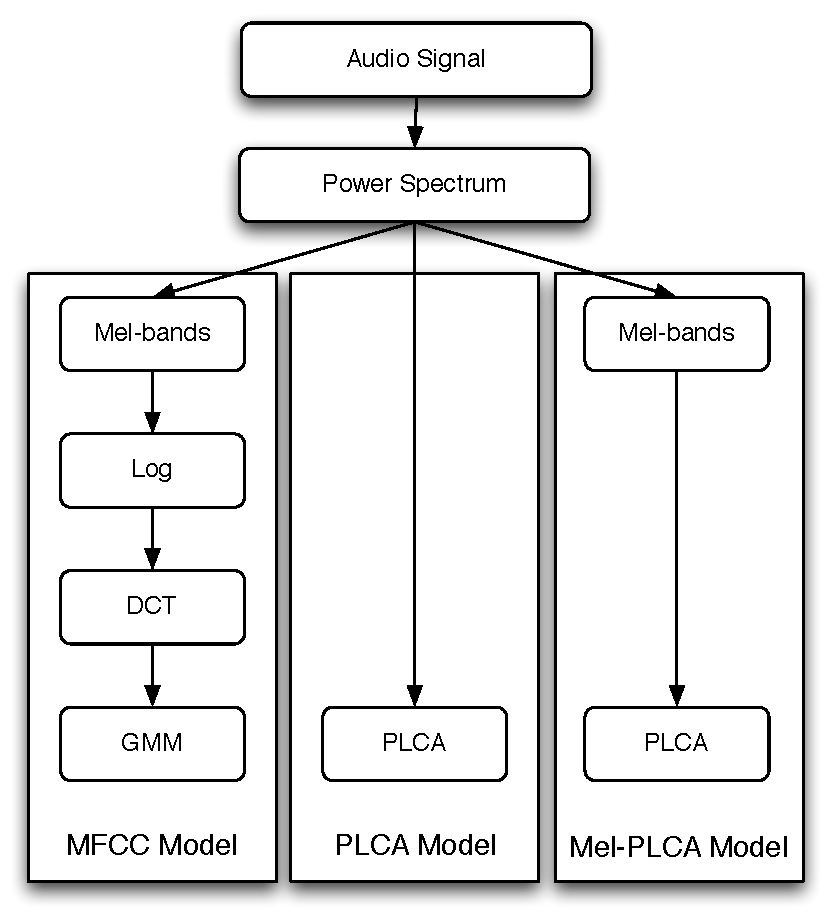
\includegraphics[width=0.99\textwidth]{images/models.pdf}
\caption{Overview of the different models}
\label{fig:models}
\end{figure}

We tested 3 kinds of models, (1), a Gaussian Mixture Model of Mel-Frequency Cepstral Coefficients (MFCC Model), (2), a probabilistic Latent Component Analysis of a frequency transformation (PLCA Model), and (3), a probabilistic Latent Component Analysis of a Mel-frequency transformation (Mel-PLCA Model).  In the following section, the models are explained in more detail.  The models are also summarized graphically in Figure \ref{fig:models}.


\subsubsection{Experiments}
\paragraph{Experiment 1}
Most previous studies in acoustic classification use multiple examples of a single class in isolation.  However, as our investigation focused on classification performance during mixtures of classes, we only trained a single example of each class, building a set of 37 classifiers for experiment 1.  As a sanity check, we tested whether the MFCC and PLCA models were able to correctly classify the test example built using the 37 classifiers.

\paragraph{Experiment 2}
For experiment 2, we determined whether the MFCC and PLCA models were able to correctly classify the trained class in the presence of an untrained class (noise).  As we have 37 classes, this equates to 36 possible mixtures for each class, where each of the 36 classes are trained in isolation, and tested in a mixture of a 37th untrained class.  In order to create the $37*36 = 1332$ possible mixtures, we used balanced mixing.  For this experiment, this means each class is actually represented with 36 possible examples (36 possible mixtures for each class).  

\paragraph{Experiment 3}
For experiment 3, we added the 37th un-trained class to the set of possible classifiers in order to see if both classes could be correctly classified when presented as an acoustic mixture.  This means we tested on $37 \choose 2 = 666$ possible mixtures and sought to find out whether the MFCC and PLCA models were capable of classifying either or both of the mixed acoustic classes, even though they were presented as a single acoustic stream.


\subsubsection{Validation and Reporting}
\label{sec:ROC}
We performed k-fold cross-validation using 10-folds.  With 10 seconds per class (370 seconds total), this equates to 1 second folds per class where training occurs on 9 seconds of material per class, and testing occurs on 1 second of material per example. The results of all folds were then averaged together to produce a single estimation.

In order to assess the estimated results, we made use of a standard technique in describing classification performance, the Receiver Operator Characteristic (ROC) curve.  ROC analysis describes ground truth classes as true and false and the predicted measures as positive and negative for a binary classifier.  The ROC curve then measures the accuracy of the classifier in separating the actual true class from the non-classes by relating the sensitivity, or the \textit{true positive rate}, against 1$-$specificity, or the \textit{false positive rate}.   In order to build the curve for a continuous classifier, the classifier's response must be converted to a set of binary classifiers by using equally spaced thresholds.  We did this by taking equally spaced thresholds on the results of our cross-validation, and calculating the true positive rate of a bin $i$ as: 

\begin{equationb}
\text{TPR}_i = \frac{\text{TP}}{\text{TP} + \text{FN}}
\end{equationb}

and the false positive rate as: 

\begin{equationb}
\text{FPR}_i = \frac{\text{FP}}{\text{TN} + \text{FP}}
\end{equationb}

The resulting $(x,y)$ points relating the false positive rate to the true positive rate are plotted for each classifier.

A perfect score is denoted by 100\% sensitivity (no false negatives) and 100\% specificity (no false positives) and corresponds to a point in the top-left corner, (0,1).  A classifier that performs at chance lies along the diagonal going from the bottom-left to the top-right corner.  

As well, the area under the ROC curve (AUC) neatly summarizes the performance of the curve with 1.0 being a perfect score, and 0.5 being a classifier that performs at chance.  We can also understand the AUC as the probability of classifying a randomly chosen positive instance with higher likelihood than a negative one.

\subsubsection{Results}

\paragraph{Experiment 1: Classifying isolated acoustic textures}

We tested the performance of a single class in isolation as a sanity check, and as we expected, the performance of the MFCC and PLCA models as determined by the ROC analysis are excellent, with an AUC of within 0.001 of perfect discrimination.

%performance during sound classification of 37 classes 
%	- handle different amplitudes
%	- microphone dynamics? 
%	- similar classes? 

%As we'd expect, the performance of both the MFCC and PLCA models perform with a perfect AUC.  

%GMM-MFCC: 98.4\%, PLCA-1c: 78.1\%

\paragraph{Experiment 2: Classifying acoustic textures in the presence of noise}

\begin{figure}
\centering
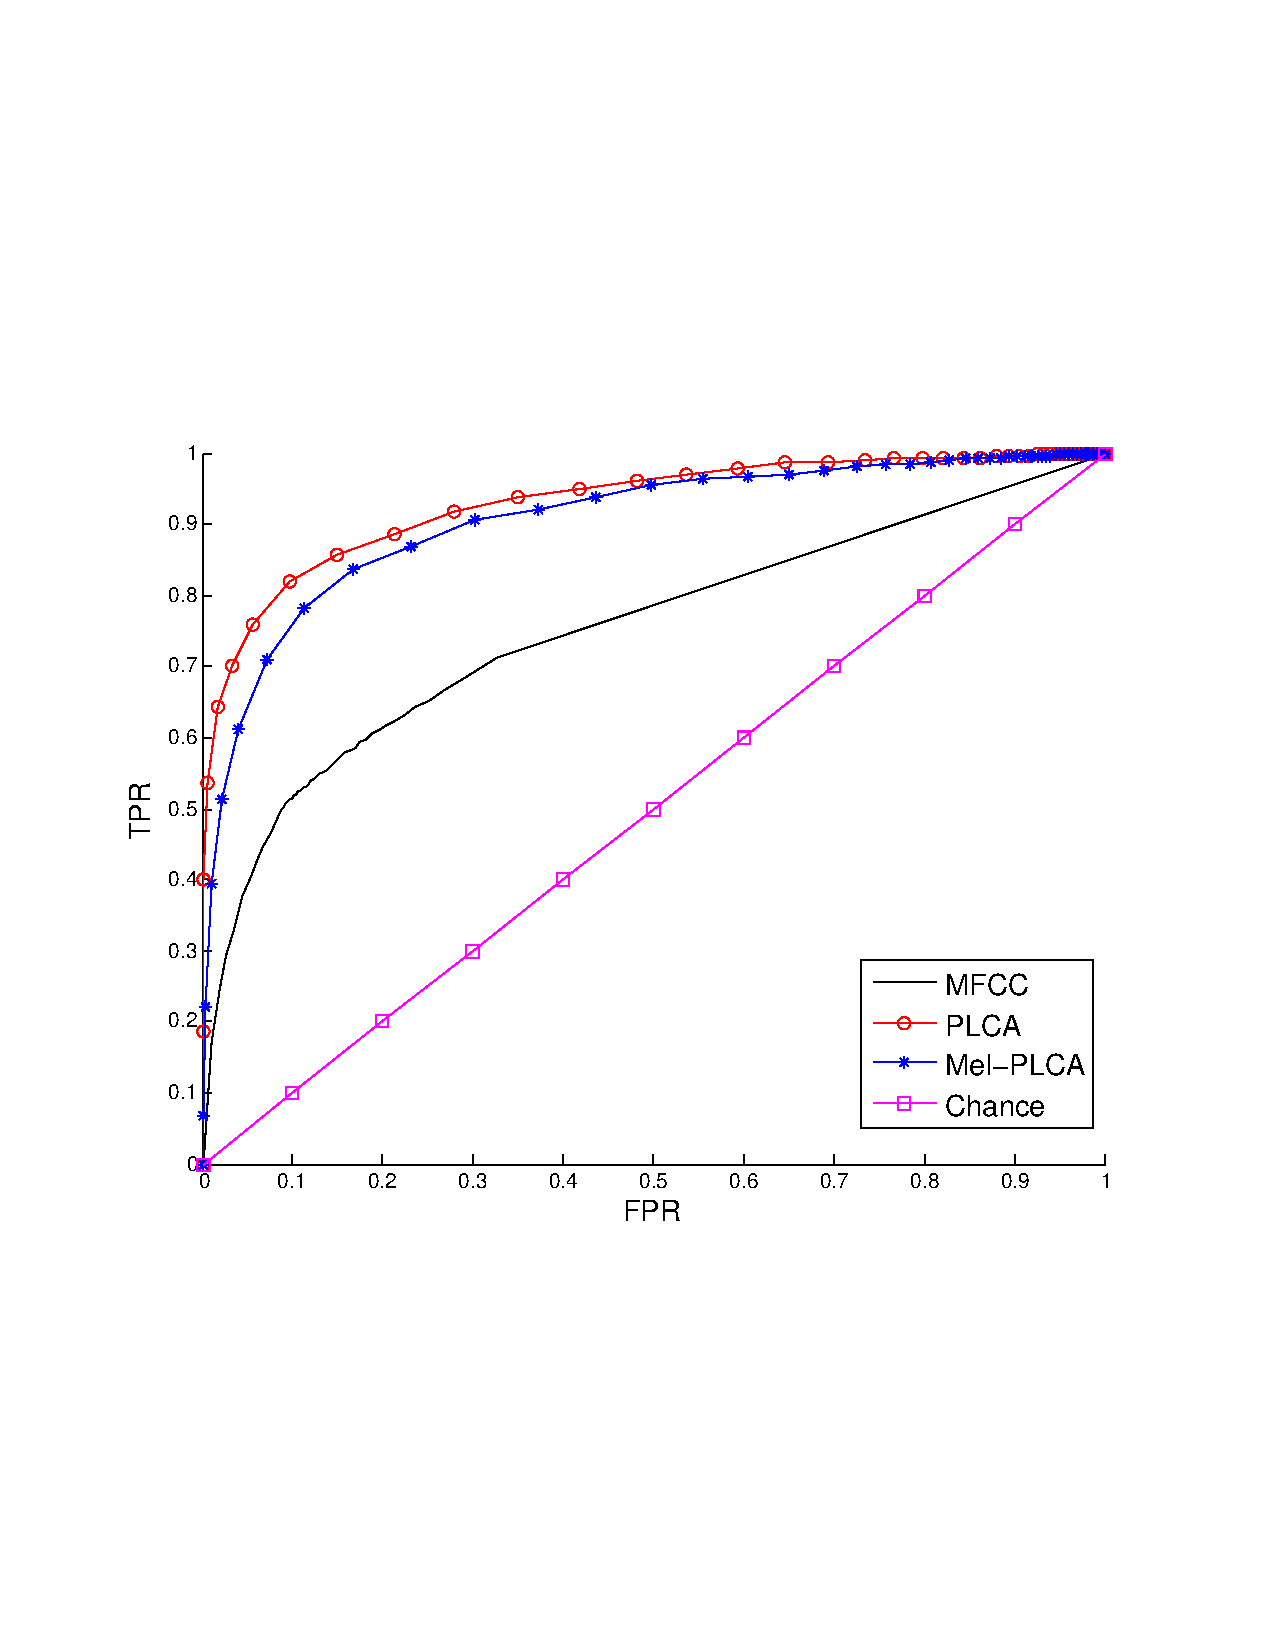
\includegraphics[width=0.99\textwidth]{images/unknown-mixture-roc-results.pdf}
\caption{Experiment 2: Classification masked by noise.}
\label{fig:unknown-mixture-roc-results}
\end{figure}

We tested the performance of both the MFCC and PLCA-based classifiers in the presence of noise by mixing one of 36 trained classes with an untrained class of sound (the 37th class), effectively masking the trained class with noise.  The average results of 1332 mixtures are depicted in Figure \ref{fig:unknown-mixture-roc-results} using ROC curves depicting each model's performance in classifying the correctly masked class.  We can see the MFCC model does well above chance, though both of the PLCA models do a far greater job.  Interestingly, the Mel-PLCA model is very close to the performance of the full-spectrum based PLCA model, even though this model uses only 40 samples versus 8192 samples per frequency frame.

\paragraph{Experiment 3: Classifying acoustic mixtures}


\begin{figure*}
\centering
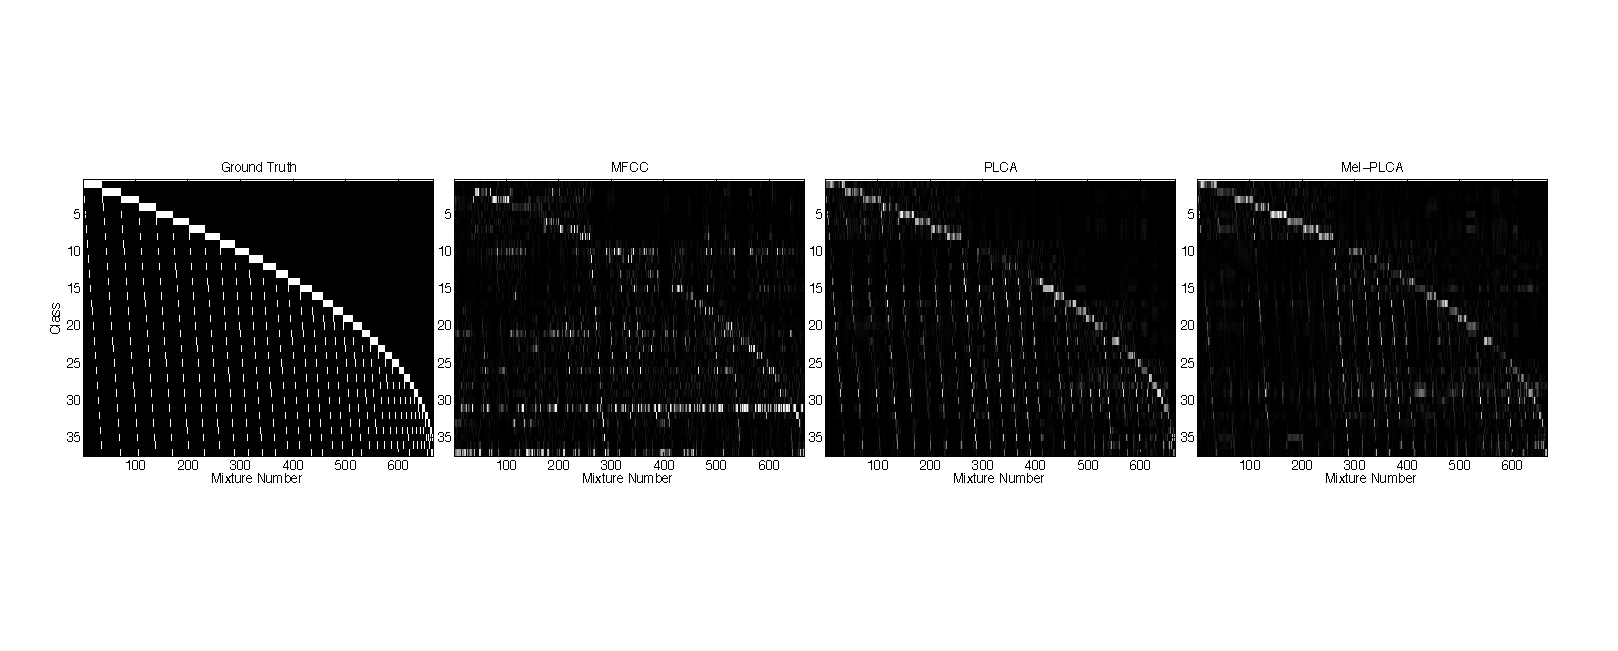
\includegraphics[width=0.99\textwidth]{images/mixture-img-results.pdf}
\caption{Experiment 3: Classification performance of acoustic mixtures depicting the ground truth classes for each of the 666 mixtures and the MFCC model, the PLCA model, and the Mel-PLCA model's classification likelihoods for each of the 666 mixtures. Images represent likelihood of a class in a given mixture, with white being 1.0, and black being 0.0.}
\label{fig:mixture-images}
\end{figure*}


\begin{figure}
\centering
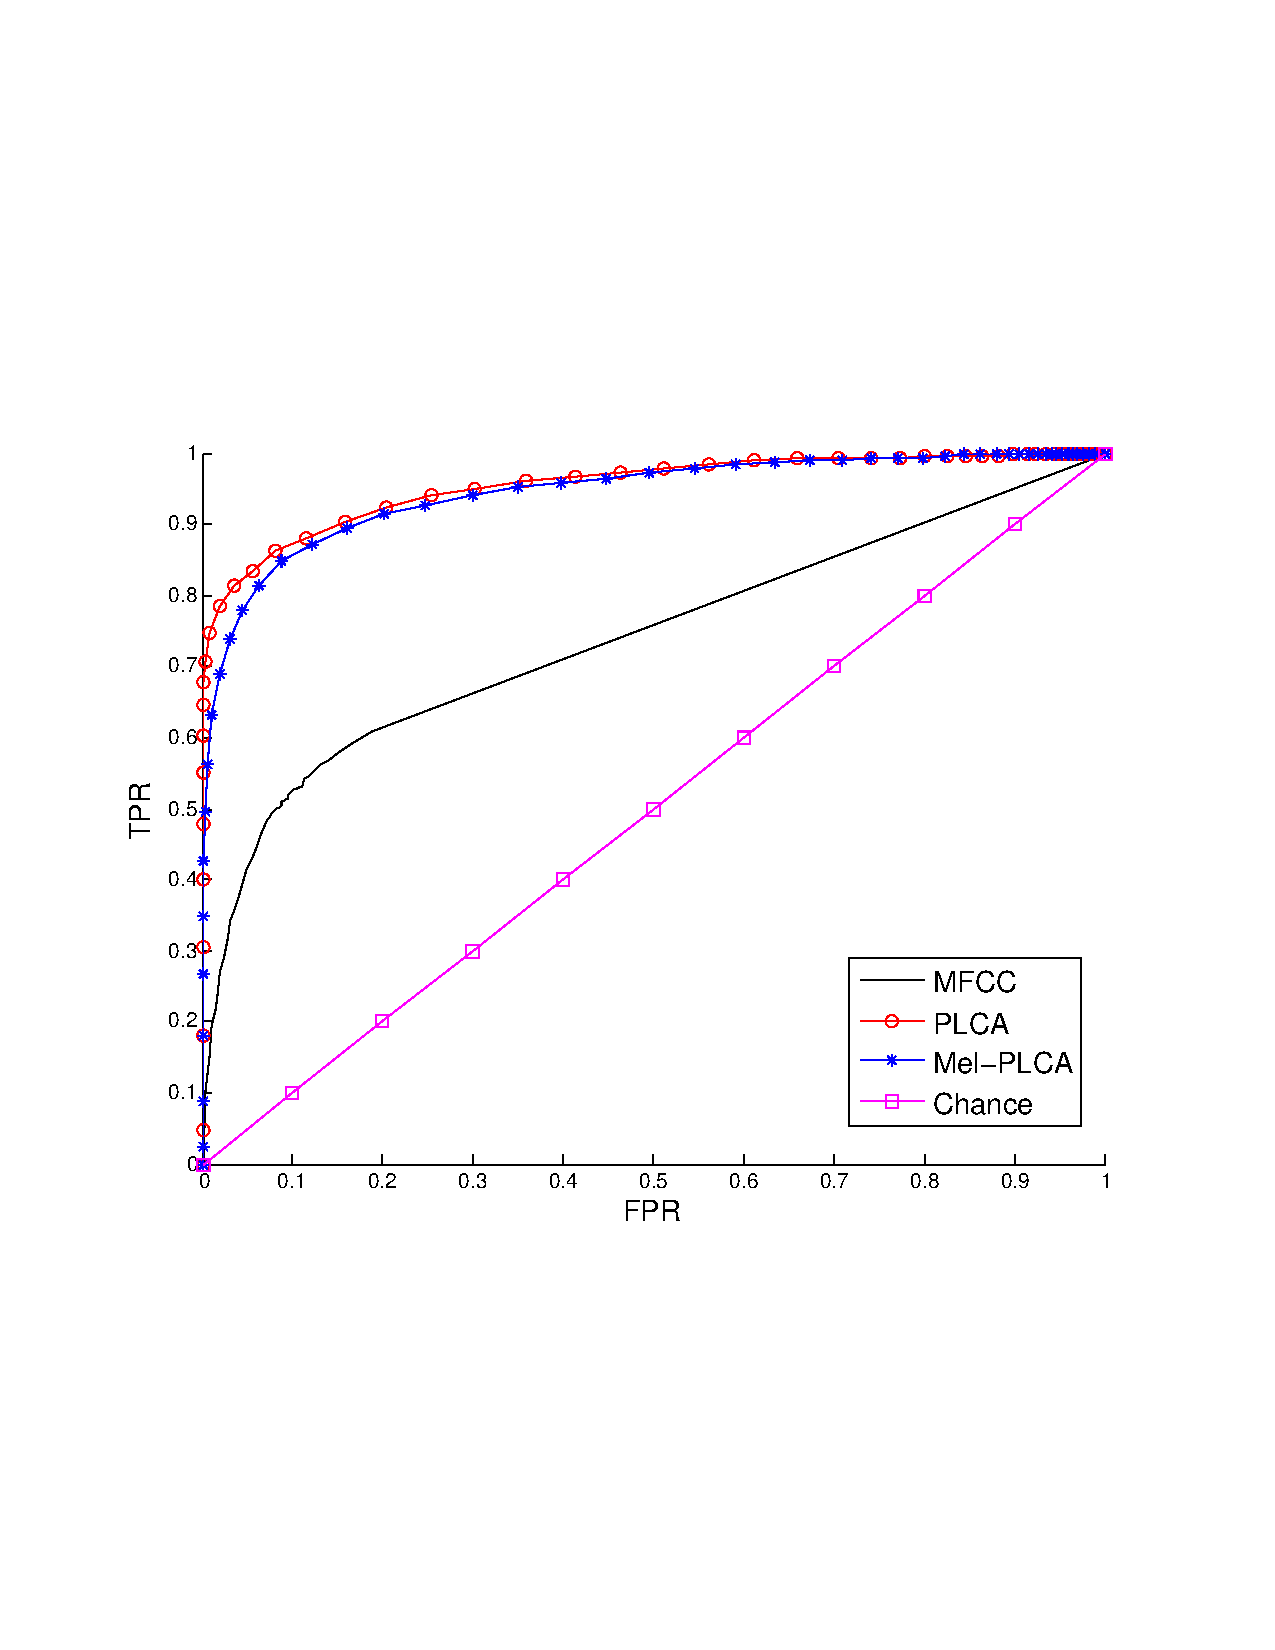
\includegraphics[width=0.99\textwidth]{images/mixture-roc-results.pdf}
\caption{Experiment 3: Classification of acoustic mixtures.}
\label{fig:mixture-roc-results}
\end{figure}



The last test we performed measures the performance of our 3 models to classify both classes in an acoustic mixture of 2.  The results depicted in Figure \ref{fig:mixture-images} show the ground truth for the 37 possible classes across all 666 mixtures ($37 \choose 2 = 666$ classes) as an image.  As well, this figure shows the likelihoods assigned to each of the 37 classes across all 666 mixtures for each of the 3 models.  From these figures, we can see the performance of the MFCC model struggles to classify most of the mixtures accurately, and often produces a false positive for classes 10 (conversation), 21 (laughing-man), and 31 (sword).  Thresholding columns of this image and storing the $TPR$ and $FPR$ as described in Section \ref{sec:ROC} produces 666 ROC curves.  The average of these curves are depicted in Figure \ref{fig:mixture-roc-results}, showing the performance of the MFCC model to be well above chance, though with the PLCA and Mel-PLCA models doing far better.  Interestingly again, we find the Mel-PLCA model is able to perform nearly as well as the PLCA model, performing within 0.01 of the PLCA model's AUC.  


\begin{table}
\centering
\caption{Area Under the Curve of ROC Analysis}
\begin{tabular}{|c|c|c|c|l|} \hline
Method&Experiment 1&Experiment 2&Experiment 3\\ \hline
MFCC&\textbf{1.0}&0.7388&0.7410\\ \hline
PLCA&\textbf{1.0}&\textbf{0.9303}&\textbf{0.9548}\\ \hline
Mel-PLCA&0.9989&0.9065&0.9443\\ \hline
\end{tabular}
\end{table}

% The methods presented can be extended to do generalizable acoustic event classification by training multiple classifiers representative of the variety of events that describe each class.  However there are three issues with any solution based purely on frequency information.  First, there is a dependence on microphone responses.  As microphone responses create a filter on the frequencies able to be represented, determining events on a headset quality microphone using classifiers trained on a studio quality microphone will be very difficult.  Second, different compression rates will also affect the representation of frequency bands creating artificial banded filters.  Lastly, how sounds may be recorded will also create ``filters'' of sound that can affect the representation of frequencies describing a sound.  For instance, in comparison to sounds heard in front of a listener, sounds heard behind a listener have a ``low-pass'' filter on the frequency responses.  


\section{Discussion}


We tested the performance of 3 types of acoustic classification algorithms, 1 based on MFCCs and 2 based on pLCA.  All 3 models performed with excellent results when a single acoustic class appeared in isolation.  However, our interests were in how such models performed when classifying the \textit{parts} that make up an acoustic scene.  We therefore devised two additional experiments: Experiment 2 masked a known acoustic class by an unknown acoustic class, effectively adding noise; and Experiment 3 tested the performance of each model to classify multiple parts of an acoustic scene by mixing 2 classes together.  The MFCC model performed well above chance in both cases with an AUC of ~0.74, but the models built on pLCA performed with much stronger results, exhibiting > 0.9 AUC in both experiments.  

One possible reason for the poor performance of MFCCs during classification of mixtures is the signal model assumes a single excitation source (e.g. vocal tract or instrument).  In the presence of multiple sources then ambiguity is created, and it becomes difficult to estimate which source contributes to each of the coefficients, especially since the sources are also combined non-linearly through the step of a log-transformation. 

Two disadvantages of using a full and direct spectrum model such as our ``PLCA model'' noted by \cite{Casey2001a} is their inconsistency and dimensionality.  We therefore tested a second model similar to the MPEG-7 spectral basis decomposition described in  \cite{Casey2001a}, ``Mel-PLCA'', which reduced the 16384 point Fourier spectrum to a 40 element vector.  However, unlike the MPEG-7 spectral basis decomposition, we made 2 significant changes: (1) we make use of the Mel-frequency scale rather than log-decibel scaling and normalization; and (2), as the article in question was written nearly 12 years ago, the only basis methods described were SVD/ICA/ and PCA based methods as PLCA had not yet been published.  Incorporating these changes, we found that the Mel-PLCA model performed within 0.03 of the full-spectrum PLCA model.  Using the critical bands defined by the Mel-frequency scale ensures the inconsistencies that may be apparent within similar acoustic classes are averaged out, and perceptually relevant frequency dimensions describing the class are retained while keeping dimensionality very low.  

\section{Future Work}

This work presents an early prototype of a broader framework capable of acoustic source separation and classification for content-based information retrieval.  A number of viable extensions are possible.  First, as we only made use of highly textured atmospheric sounds, it remains to be seen whether the following method alone would suffice in modeling more impulsive sounds, e.g. drums, birds, or less atmospheric sounds.  In such cases, an entropic prior on the temporal weights of a pLCA decomposition would very likely greatly improve results \cite{Smaragdis2007}, ensuring the sparsity of temporal weights in the latent distribution $p(t|k)$, while capturing the bulk of the frequency distribution in the latent factor $p(f|k)$. 

Second, 2D patch-based and shift-invariant convolutive pLCA \cite{Smaragdis2007} has shown great promise in capturing the structure of music when applied to chromagram features and when using sparsity and shift-invariance in all features \cite{Weiss2011}.  Such a technique has the power not just for classifying the instruments that describe a musical passage, but as well the course of events that describe the musical scene, essentially identifying whole musical passages or riffs.  

Third, In real-time scenarios, it is often the case that a dictionary of classes is not readily available.  Recent work describing the online-learning of dictionary elements using pLCA has shown great promise in performing real-time speech de-noising \cite{Duan2012}, resulting in components separating noise and speech.  Such a distinction has wide applications in fields such as surveillance and tele-presence technologies.  

Lastly, in developing this work, it became apparent that no standard publicly and freely available libraries for evaluating acoustic-based CBIR algorithms exists.  Though the problem is well noted in music information retrieval \cite{Casey2008b,Rhodes2010}, and recently addressed with databases such as the million song dataset \cite{Bertin-Mahieux2011}, no standardized databases have been developed as freely available archives in the general sound-based multimedia communities.  As such, testing the scalability of our approach proved very difficult, as we could only obtain 37 classes and a total of 1332 mixtures even though databases such as Youtube and typical multimedia archives are on the order of many millions.  Future work must therefore be done to help understand the scalability and performance across different approaches using a standardized database.  

assumptions in what is segregated... should have used people .. .but even subjective no good... rep...


\section{Conclusion}


%%%%%%%%%%%%%%%%%%%%%%%%%%%%%%%%%%%%%%%%%%%%%%%%%%%
%%%%%%%%%%%%%%%%%%%%%%%%%%%%%%%%%%%%%%%%%%%%%%%%%%%
%%%%%%%%%%%%%%%%%%%%%%%%%%%%%%%%%%%%%%%%%%%%%%%%%%%
%%%%%%%%%%%%%%%%%%%%%%%%%%%%%%%%%%%%%%%%%%%%%%%%%%%
%%%%%%%%%%%%%%%%%%%%%%%%%%%%%%%%%%%%%%%%%%%%%%%%%%%
%%%%%%%%%%%%%%%%%%%%%%%%%%%%%%%%%%%%%%%%%%%%%%%%%%%
%%%%%%%%%%%%%%%%%%%%%%%%%%%%%%%%%%%%%%%%%%%%%%%%%%%



%%%%%%%%%%%%%%%%%%%%%%%%%%%%%%%%%%%%%%%%%%%%%%%%%%%
%%%%%%%%%%%%%%%%%%%%%%%%%%%%%%%%%%%%%%%%%%%%%%%%%%%
%%%%%%%%%%%%%%%%%%%%%%%%%%%%%%%%%%%%%%%%%%%%%%%%%%%
%%%%%%%%%%%%%%%%%%%%%%%%%%%%%%%%%%%%%%%%%%%%%%%%%%%
%%%%%%%%%%%%%%%%%%%%%%%%%%%%%%%%%%%%%%%%%%%%%%%%%%%
%%%%%%%%%%%%%%%%%%%%%%%%%%%%%%%%%%%%%%%%%%%%%%%%%%%
%%%%%%%%%%%%%%%%%%%%%%%%%%%%%%%%%%%%%%%%%%%%%%%%%%%




\chapter{Computational Auditory Scene Synthesis}
\label{ch:synthesis-audio}
\minitoc

%\section{Abstract}

%Memory Mosaicing is a real-time sonic collage experience employing a perceptually-motivated model for representating and attending to sounds. This model relates the ongoing auditory world to previously learned ``sonic memories''.  Using a mobile platform, a user of the system wears earphones listening to an augmented sonic world which relates the incoming microphone stream to previously segmented sound clips, or sonic memories, creating a ongoing mosaic of sonic memories.  The system starts with an empty knowledge-base of sounds and continually stores only the segments of sounds which are determined salient and unclassified by a machine listening model.  The engine for synthesis is concatenative, matching the incoming segments to the learned ''sonic memories''.  The experience works in real-time on an iPhone 3 and above and has interactive parameters controlling the synthesis engine as well as the ability to learn from the user's own music library.  The experience of the iPhone app is multi-fold, creating a novel platform for investigating the role of memory in perception or as compositional or performance tool which grows its own expressive capabilities the more it hears.

\section{Introduction}

perceptual model of listening to help determine the representation of the corpus... daphne oran browser.


The juxtaposition of fragments of sound as an arts practice has roots at least as early as music concrete, a compositional technique assembling various natural found sounds in order to produce a collage of sound.  Digital Sampling came in the 1970's allowing sound segments to be triggered using an interface such as a keyboard or pad.  More recent techniques have focused on corpus-based concatenative synthesis, where a target sound is matched to a stored database of segments or sounds (for a comprehensive review, see \cite{Schwarz2006}).  

This chapter focuses on describing practical outputs in developing auditory scene synthesis.  The culmination of this practice will lead to the development of an application, ``Memory Mosaic'', which delivers an automated sonic-collage to a single user wearing headphones.  This application will also later be used in combination with the developments in my visual-practice in Chapter 7.   Before developing this application, however, I will discuss a few outputs created along the way which focused on exploring the use of spatialization, cut-up, narrative, and memory within a sonic collage practice.  

\section{Sonic Graffiti}

The first practical output I developed towards building an auditory scene synthesis is an application called ``Sonic Graffiti''.  The aim of this application was to create a soundscape based on a collage of sounds that had been recorded at different locations in 3-dimensional space.  A participant of the application could record sounds whenever they pressed a button and could do so in different locations in 3-dimensional space.  Then, when the participant would move in space, they would be able to hear the sounds they recorded as a continuous loop coming from the original location that they were recorded.  The interest in developing this application was (1) to synthesize an acoustic scene by replaying sound fragments based on their original location in space, and (2) to discover more about 3-dimensional sound perception.  My target platform at the time of development was the Apple iPhone 4, which includes a GPS sensor, digital compass, microphone, and audio output.  To begin with, I needed to discover how to record a set of sounds that could be re-positioned based on how a user moved around in 3-dimensional space.

\subsection{Methods}

\subsubsection{3-dimensional Sound Perception}\label{sec:binauralization}
To recreate the perception of a recorded sound as coming from a particular location in 3-dimensional space, one could record the sound using a binaural microphone.  These are a stereo pair of microphones (2-channels) which are placed in each ear and capture the sound as it would ideally enter your own ears.  When the captured sound is played back through headphones, they should sound fairly realistic creating the impression that a sound had originated in the same relative location to the user.  However, at the time of developing ``Sonic Graffiti'', the iPhone 4 did not support recording of more than one channel of sound without the support of an external device, meaning a binaural microphone would not work.  As a result, I investigated other methods for spatialization which could work with monaural sounds.

One convincing feature of the perception of 3-dimension sound is the Interaural Time Lag (ITL), the lag in time of a sound reaching either ear.  If a sound reaches my left ear faster than my right ear, I perceive a sound coming from the left side of me.  Similarly, if it comes to my right ear faster than my left, then I perceive it as coming from the right of me.  But what about a sound directly in front of me or directly behind me?  These should have the same ITL, though if you listen to a sound behind you, you may notice that higher frequencies are harder to hear.  This is due to the shape of your ear blocking direct waves from entering your earlobe.  Instead, they must travel around or through your ear, creating both an attenuation and a low-pass filter, similarly to what a thin wall may do in effect.  

One could model the perception of sound in 3-dimensions using a set of rules for creating time-lags and filtering sound based on its back-to-front position.  However, another method is to create a sampling of sounds from all directions around an actual head and use these recordings to understand how sound is filtered from any direction.  IRCAM's LISTEN database achieves this by providing a set of Head Related Impulse Responses.  This library has a large database of recordings that was built as follows: using an anechoic chamber, a space where acoustic foam is placed on the sides of the wall in an effort to minimize any reverberations of sounds, a user was sat in the middle of the space.  Within their ears, microphones were placed.  A speaker was moved at a spherical distance 1.95 meters away from the user and produced a ``click'': an instantaneous change in pressure perceived as a loud ``pop'' without any reverberations.  This click essentially delivers a sound wave reaching either ear with an interaural time lag and filtering based on the speakers relative location to the user's head.  

\begin{figure}
        \centering
	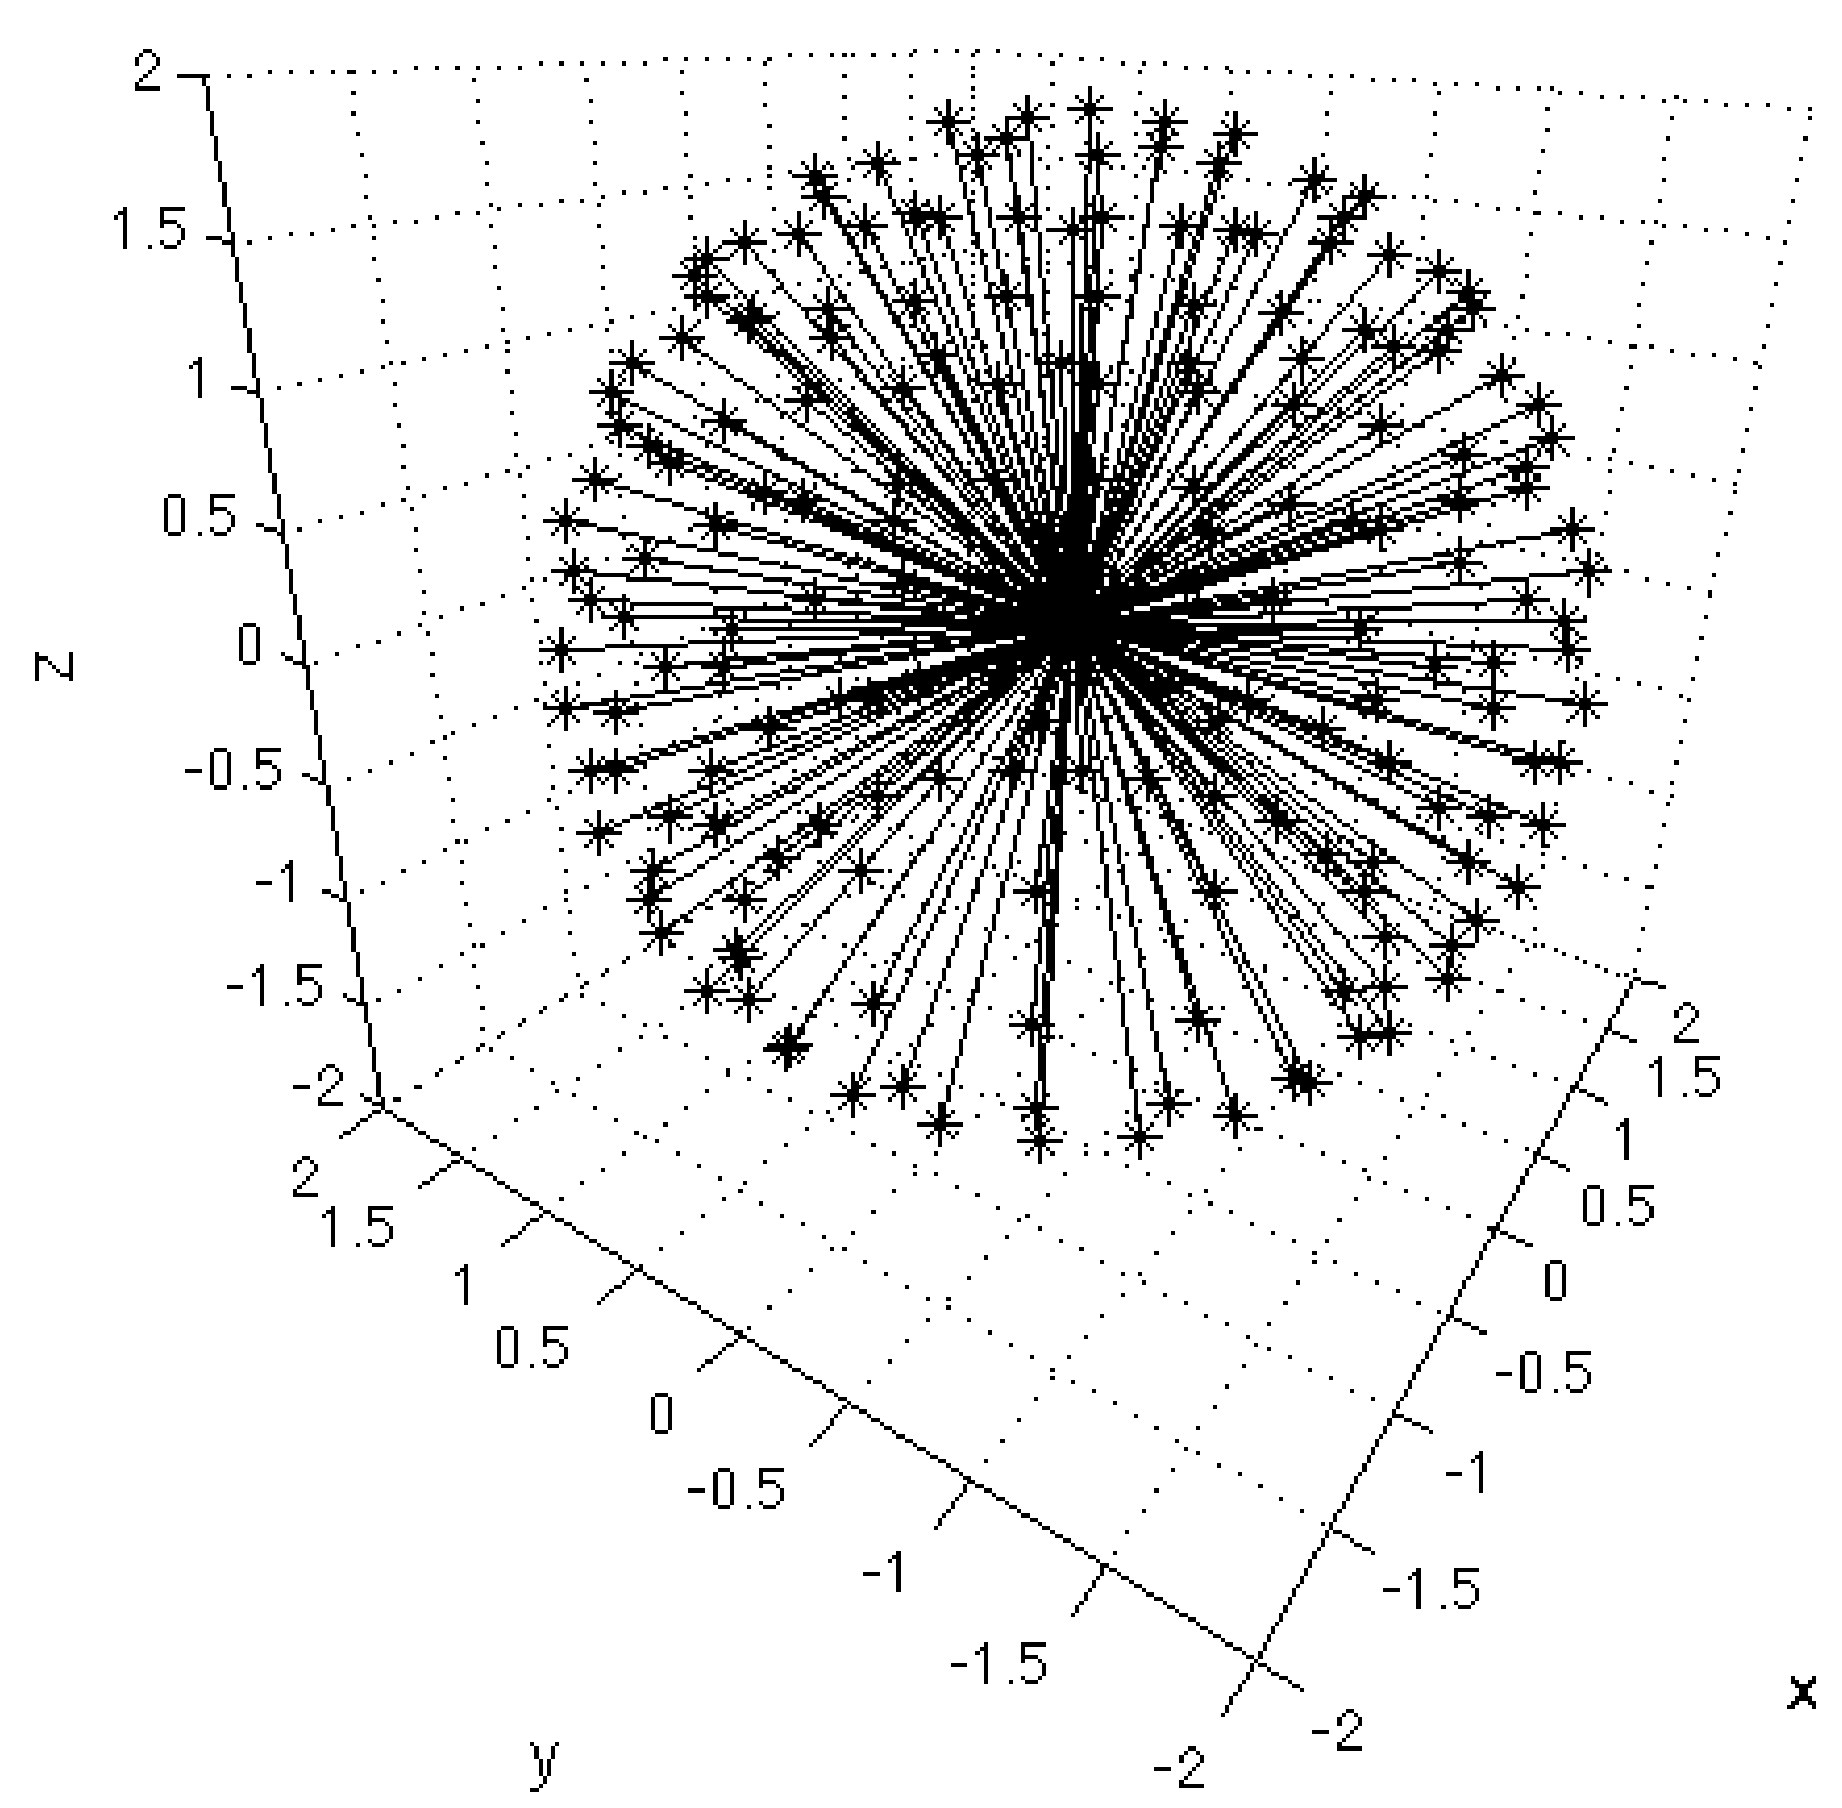
\includegraphics[width=\textwidth]{images/sphere-xyz-01.png}
	\caption{Locations of all 187 Head Related Impulse Responses relative to the user's head.}
	\label{fig:ircam-listen}
\end{figure}
                
\begin{figure}
        \centering
        \begin{subfigure}[b]{0.49\textwidth}
                \centering
                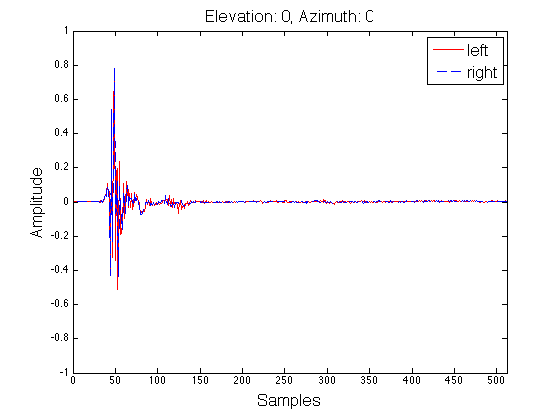
\includegraphics[width=\textwidth]{images/el0-az0.png}
                \caption{Front}
                \label{fig:gull}
        \end{subfigure}%
        \begin{subfigure}[b]{0.49\textwidth}
                \centering
                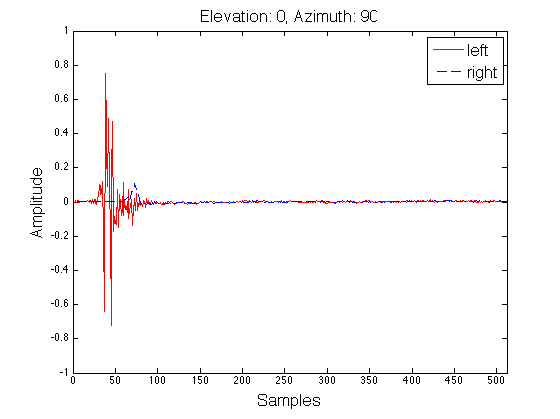
\includegraphics[width=\textwidth]{images/el0-az90.png}
                \caption{Left}
                \label{fig:tiger}
        \end{subfigure}
        \begin{subfigure}[b]{0.49\textwidth}
                \centering
                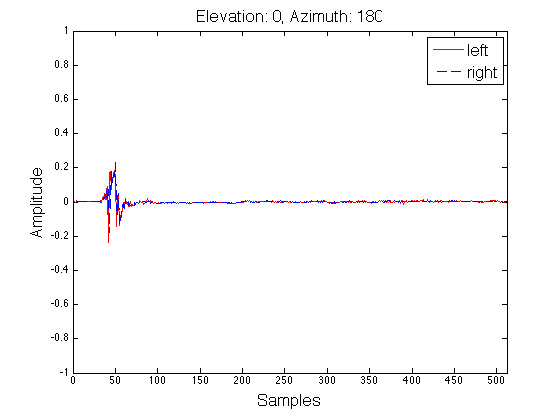
\includegraphics[width=\textwidth]{images/el0-az180.png}
                \caption{Behind}
                \label{fig:mouse}
        \end{subfigure}
        \begin{subfigure}[b]{0.49\textwidth}
                \centering
                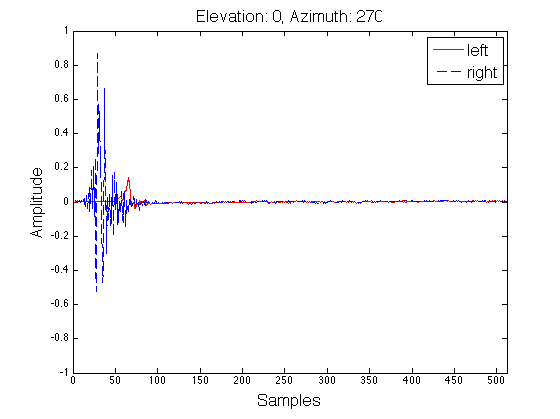
\includegraphics[width=\textwidth]{images/el0-az270.png}
                \caption{Right}
                \label{fig:mouse}
        \end{subfigure}
        \caption{Example signals for the Head Related Impulse Responses of 4 different positions.}\label{fig:ircam-hrir}
\end{figure}

The IRCAM LISTEN database comes with 71 sets of 187 recordings, where each set comes from a different participant, and thus has slightly different responses (due to the individual features of their head, such as the shape of their ear or nose) .  Each recording is 8192 samples long at 44100 Hz sample rate.  Figure \ref{fig:ircam-listen} depicts the locations of all the ``clicks'' in relation to the user's head while Figure \ref{fig:ircam-hrir} depicts 4 filters from a single individual's recordings, IRCAM 1087, from an elevation equal to the individual's ears and placed to the front, left, back, and right of the center of the head at a distance of 1.95 meters away.  Using all 187 recordings gives a reasonable sampling of the space around a user's head, creating a set of ITL's with known relative locations.  Thus, any sound can be binauralized by using any of the 187 recordings.  However, as these are all spaced at 1.95 meters away from the user's head, a sound that is closer or farther away than 1.95 meters must be attenuated.  Further, these 187 sampled locations must be converted to a continuous sampling, allowing for a sound to be binauralized anywhere on surface of a sphere, through the use of interpolation.  To achieve both of these extra features, I use a k-Nearest Neighbor tree using the 3 closest neighbors to a point on a sphere.  These three nearest points are then averaged to produce the final left and right ear filters.  The average distance to the nearest filters are used to attenuate the final filter using a logarithmic relationship between distance and attenuation, simulating the logarithmic perception of sound (decibels).

Any incoming sound may then be filtered using the final combined and attenuated filter.  To filter the original sound with the binaural filters, we make use of an FFT-based convolution to filter the original sound with the binaural filters.  We first remove most of the silence from all filters, cropping the original 8192 sample filters to 512 samples.  Then, an incoming sound wave is chunked in 512 sample frames.  The resulting convolution of the original frame and the filter is $(2N + 1)$ samples long. To achieve continuous filtering, we use an overlap-add operation.  Overlap-add takes the additional resonance, or the additional 513 samples as a result of the convolution operation, and adds this as an overlapping part to the next frame of filtering.  This ensures any energy in the system is continuously kept in the filtering procedure.  

\subsubsection{GPS}

A user's location is obtained using Apple's CoreLocation framework.  This provides a latitude, longitude, and altitude using Global Positioning System (GPS).  As this defines a point on a Earth through a spherical coordinate system, this location must be converted to a 3-dimensional cartesian point to be used with the filter tree in Figure \ref{fig:ircam-listen}.  For this purpose, a specific projection which flattens the Earth's surface to a 2-dimensional landscape must be used.  We make use of the Universal Transverse Mercator (UTM) coordinate system which maps latitude and longitude locations to a mercator projection, and is described in detail in the 330-page document, Bulletin 1532, by the United States Geological Survey \cite{}.  Any new ``graffiti'' is then given the user's current UTM $x,y$ and altitude.  

CoreLocation also provides different modes of accuracy depending on the application's needs.  As ``Sonic Graffiti'' requires a high precision of accuracy, this was set to ``kCLLocationAccuracyBestForNavigation'', which the Apple Developer Documentation\footnote{\url{https://developer.apple.com/library/mac/documentation/CoreLocation/Reference/CoreLocationConstantsRef/Reference/reference.html#//apple\_ref/c/data/kCLLocationAccuracyBest}} describes as:
\begin{quotationb}
Use the highest possible accuracy and combine it with additional sensor data. This level of accuracy is intended for use in navigation applications that require precise position information at all times and are intended to be used only while the device is plugged in.
\end{quotationb}
During the development of this application, it was found that accuracy when not moving was unreliable to at least 10 meters.  When moving, however, particularly in a straight line, accuracy was more reliable, perhaps to within 1 meter.  As an example, the plots in Figure \ref{fig:gps-tracking} show two example paths taken by me walking around a single block in London.  

\subsubsection{Sonification}

The resulting sonification of any recorded graffiti is achieved through (1) discovering the relative position of the graffiti to the user's current location and orientation, (2) binauralizing the individual graffiti using the procedure described in Section \ref{sec:binauralization}, resulting in a stereo audio signal, (3), summing all resulting binauralizations, and (4) mixing the resulting stereo sum using a compressor so that the signal is within the speaker's limits.   

During initial tests, only 2 - 3 sounds could be binauralized at a time, before clicks and buffer underruns occurred.  These are typical signs that a CPU cannot keep up with processing and is instead opting out of processing audio for a few frames until processing can catch up.  

\subsubsection{Vectorization}

In order to increase the number of sounds that could be binauralized without CPU lags, we made use of vector-based acceleration.  This is a technique that takes advantage of large register sizes in CPU architecture, in this case 16-bytes.  Instead of performing an operation on a single byte, or in the case of floating-point data, 4 bytes, the same operation may be performed on 16-bytes using larger registers.  Further, if the amount of memory is fixed to a certain size, for-loops which require branching on each iteration may be sacrificed through the use of larger register operations, requiring far less branches.  These optimizations are cleverly implemented in the Apple Accelerate Framework, making many arithmetic operations very fast to perform.  After rewriting the binauralization routines in Accelerate language, I could binauralize 25-30 sound sources before clicks and buffer underruns occurred. 

\subsection{GUI}

\subsection{Discussion}

Sonic Graffiti allows a user to record a sound based on the current GPS location of the device.  The resulting sound is played back as a continuous loop and spatialized based on the user's relative location to the original recorded location.  This is achieved through the use of a bespoke binauralization library.  As the routines require significant processing as the number of sounds increase, vectorization was used to accelerate computation.  The resulting framework has been made available online for anyone to use at \url{http://github.com/pkmital}.

\section{Future Echoes}

Next are two installation outputs developed as part of a course I led in a design school in India which explore the use of cut-up technique in delivering a spatialized sonic narrative and the use of sound input as a target for a video-based triptych collage.  

\subsection{Ambisonics}




\subsection{Browser}

\subsubsection{Introduction}
We focus on visualizing the Daphne Oram archive using two methods for describing the archive: (1) discovering latent distributions of frequencies using a recently developed source separation algorithm, probabilistic latent component analysis (PLCA) \cite{SmaragdisRajShashanka}; and (2), using a widely-adopted multi-dimensional feature for speech, music, and general acoustic classification, the Mel-Frequency Cepstral Coefficients (MFCCs).  We cluster the data from either descriptor using Multidimensional Scaling and develop a 3D visualization that allows researchers to project the archive onto multiple dimensions of the data.  Finally, we report user-feedback from researchers of the archive using the 3D visualization tool.  

Our main contribution is in describing the impact of visualizing segregated streams of a large audio archive through a case-driven exploration of the work of Daphne Oram.  We compare the feedback from archivists using a visualization of latent timbre-relationships versus one using a perceptually inspired multi-dimensional feature, MFCCs, and show that PLCA is more effective at producing a meaningful visualization.  


\subsubsection{Browsing}

A number of previous approaches for visualizing large audio corpora have focused on the application of music-based corpora.  Some approaches to content-based musical information retrieval solutions require a user to search by example or performance, aiding retrieval when a user is unaware of exactly what they are looking for.  However, visualization of such retrieval methods often amounts to viewing lists of the $k$-most similar results of an explicit query, and thus any exploratory analysis of the corpus as a whole requires further research into approaches for visualization.  For instance, SMILE \cite{Melucci2000} presents a MIDI-keyboard for the user to ``perform'' a query, and results are presented based on how similar the MIDI sequences are to the performance.  Similar approaches built for more generic signal-based audio break a corpus into frequency information and further into fingerprints such as MFCCs or psychacoustic descriptors.  audioDB \cite{Casey2008c,Rhodes2010} for instance allows a user to input shingles, or segments of an audio track for discovering similarities in an archive.  Other solutions such as Query-by-humming allow a user to hum/sing a tune in order to discover similar results (e.g. \cite{Wang2006a,Cartwright}).  The previous methods may be suitable for applications where a user has an explicit example query.  However, in exploring an archive, it requires the user to have a priori knowledge of what the archive already contains.

Early work in exploratory content-based visualization systems can easily be traced to the 1990's where Starfields were commonly employed.  Starfields are interactive scatter-plots that allow for zooming, panning, and selection for greater detail, allowing one to view an archive through interaction.  The Informedia Digital Video Library System (1994-1998) \cite{Himmel1998,Christel1998} is one such system making use of the Starfield visualization approach, which accesses over a tera-byte of video and presents the user with an interactive scatterplot organized by the user's query.  Beginning with the audio signal, Informedia-I uses the Sphinx-II speech recognition system to discover annotations of audiovisual material.  Adding these to any existing text-annotations from captions, they create a term-document frequency matrix for each video segment, where segments are determined through the use of motion-based video-cut detection.  They are then able to discover latent relationships using PCA for reduction and visualization.  Other approaches such as IVEE \cite{Ahlberg1995} allowed for visualization options such as Tree Maps, Cone Trees, and even 3D scatterplots, though were not rooted in content-based information retrieval and instead relied on explicit relations of existing meta-data.  Though these early works were not directed for musically-based archives, their approaches towards visualization and interaction are very similar to ours, as we also look for latent relationships for reduction and visualization.

More recently, CataRT \cite{Schwarz2008} approaches Starfield style visualizations of large audio corpora by computing low-level psychoacoustic descriptors of grains segmented from a corpus for the purposes of composition, orchestration, and texture synthesis.  Visualizing the resulting mappings occurs in a 2D space where each axis is defined by a descriptor chosen by the user.  Such a visualization has the benefit of user awareness and control over the mappings that define a parametric spatial mapping.  Plumage \cite{Schwarz2008} extends the CataRT visualization into a 3D space creating a performance and composition environment where grains are colored, textured, and morphed in 3D space based on their psychoacoustic descriptions.  nepTUNE \cite{Knees2006} and \cite{Dominik2009} are two approaches to visualization which create a 3D terrain-style virtual space.  Songs are clustered using a self-organizing map of acoustic similarity in order to create virtual islands and terrain based on their clustering density.  The created virtual space thus encourages exploration and navigation of the visualized corpus.  \cite{Bartsch2001}'s approach employs the use of chroma-features for producing audio thumbnails of tracks, or segmented versions of an audio track encoding heavily repeated structures of harmonic relationships.  Though their approach is well-suited for popular music archives, they note that it is not suitable for music that does not obey a simple ``verse-refrain'' form.  \cite{Stewart2008} uses mood words to describe a 3D interactive visualization, though relies on having access to socially tagged music in order to represent the music archive.  \cite{Heise2012} use MFCCs to describe an unknown corpus of audio and explore the audio using a 2D visualization created with a self-organizing map.

The critical deviation of our approach to feature analysis from the previous approaches is by defining a 3D space using the corpora's own latent frequency distributions.  As we make no assumptions to the structure, perceptual relevance, or harmonic nature of the corpus, using probabilistic latent component analysis, we can discover the archive's own predominant distributions of frequencies and are able to use this reduced dimensionality dictionary as a representation of a high-dimensional space.  When projecting any 3-dimensions, the user is able to navigate the archive in a manner similar to CataRT \cite{Schwarz2008}. However, the axes are not user-defined psychoacoustic descriptions, but rather are projections of the archive onto ``timbres'' defined by latent frequency distributions.  Our work similarly encourages exploration and navigation as in  \cite{Knees2006,Dominik2009,Heise2012}, though takes a information-centric point of view to analysis and retrieval.   We build a second visualization using a model which does not take into account the density of the data but instead uses a perceptual frequency transformation for building decorrelated features, MFCCs, similar to \cite{Heise2012} and report the user feedback for each visualization.

\subsubsection{Method}

Currently, the Daphne Oram Archive has over 215 tape reels or 60 hours digitized.  As the amount of available memory is a constraint on our approach, we are only able to investigate the first 10 minutes of the first 60 tape reels or 10 hours in total.  We describe each half second segment by their frequencies over time, described using the short-time Fourier transform, and describe each time-frequency matrix as a slice.  In total we have 1200 slices per tape and 72,000 slices for all 60 tape reels\footnote{We use all data for building the description of the corpus, though later use a reduced subset for visualization.}.  We aim to visualize this data using a clustering algorithm able to extract the timbre-relationships within the archive.  Specifically, we look at two methods for grouping the possible interesting frequencies describing the archive: (1) PLCA, a probabilistic method for discovering latent component relationships of a time-frequency matrix, and (2) MFCC, a widely-adopted approximation of the frequency spectrum inspired by the human auditory system's response properties.

\paragraph{PLCA Model}
One drawback with the basic PLCA model is the number of components describing a distribution must be known \textit{a priori}.  We therefore incorporate model selection, a commonly employed information theoretic approach to determining parameters of a model.  In the case of PLCA, the model parameters are described by $N$, the number of components.  To appropriately determine the correct value for $N$, we use \textit{Bayesian Information Criterion} (BIC) model selection.  Using the log-likelihood of the optimized parameters, an additional parameter which penalizes model complexity is subtracted from the log-likelihood:
\begin{eqnarray}
\ln{p(X)} &\simeq& \ln{p(\mathcal{D}|\theta_{\mathtt{MAP}})} - \frac{1}{2}M\ln{N}
\end{eqnarray}
where $M$ is the number of parameters in $\theta$ and $N$ is the number of data points.  BIC ensures that we do not let the model overfit to a large value of $N$, while still producing a suitable log likelihood explanation of the observed data.

To begin the model selection, we iterate through every slice of audio.  Using model selection, we compare the results of using the current number of components and using an additional component.  If the results are better explained with an additional component, we add one to the value of $N$ and continue to the next slice. Iteratively running PLCA across all slices on increasing values of $N$ until finding the maximum BIC results in finding $N=45$ for 10 hours of audio.  

\paragraph{MFCC Model}
For our second model, we use the commonly employed Mel-frequency Cepstral Coefficients (MFCCs) which approximates a frequency spectrum by a set of de-correlated features.  

\paragraph{Multi-dimensional Scaling}
After running each model, we are left with an $M \times N$ dimensional matrix, where $M$ refers to the number of time slices, and $N$ to the number of dimensions that describe each feature.  In the case of PLCA, after running model selection, we are left with $N=45$ dimensions describing the data.  With regards to MFCCs, we specifically choose $N=13$ cepstral coefficients.  

In order to visualize the high-dimensional space created by either model and cluster together similarly weighted features, we make use of Multi-Dimensional Scaling (MDS), a popular technique for multivariate and exploratory data analysis. MDS is a common technique for projecting data in high-dimensional spaces to 2 or 3 dimensional spaces for the purposes of visualization.  It aims to preserve the pairwise distances between data points, starting with the notion of distance, and working backwards in order to create the coordinate space.  The basic algorithm for calculating the unknown low-dimensional coordinate map $\mathbf{X}$ thus starts with a distance or proximity matrix, $\mathbf{P}$.  We aimed to use the full archive of 72,000 slices, however creating a matrix of float values this large requires $~20$ gigabytes of information which must be held in RAM.  Therefore, we reduce our database by taking every 5th slice, effectively looking at 0.5 second slices every 2.5 seconds rather than every 0.5 seconds.  However, the description of the data in the case of PLCA is still dependent on all 72,000 slices.
  
In order to calculate the low-dimensional coordinate matrix, we calculate the largest eigenvalues of the distance matrix after applying a double centering procedure.  The basic MDS algorithm is summarized as follows:
\begin{enumerate}
\item Compute a $M \times M$ proximity matrix $\mathbf{P}$ by calculating the Euclidean distances between each of the $M$ features
\item Compute the inner product matrix $\mathbf{B}$ by applying double-centring to the proximity matrix $\mathbf{P}$: 
\begin{equationb}
\mathbf{B} = -\frac{1}{2}\mathbf{J}\mathbf{P}^{(2)}\mathbf{J}
\end{equationb}
where $\mathbf{J} = \mathbf{I} - n^{-1}\mathbf{1}\mathbf{1^{\mathtt{T}}}$ and $n$ is the number of objects.
\item Compute the eigenvalue decomposition and retain the $n$ largest eigenvectors, $\mathbf{e}_1, ..., \mathbf{e}_n$ in order to compute the $n$-dimensional coordinate matrix $\mathbf{X}$:
\begin{equationb}
\mathbf{X} = \mathbf{E}_n\mathbf{\Lambda}_n^{\frac{1}{2}}
\end{equationb}
using the eigenvectors $\mathbf{E}$ and eigenvalues $\mathbf{\Lambda}$ of $\mathbf{B}$ 
\end{enumerate}

One may also notice the algorithm is equivalent to a doubly-centered version of PCA in the case where the distances are Euclidean.  As both the PLCA and MFCC model's feature dimensions are de-correlated, we would expect to find the number of eigenvalues approach the same dimensionality as either model.  Thus, the PLCA model is clustered in 45 dimensions, and the MFCC model in 13.


\subsubsection{Browser}

\begin{figure*}
  \centering
  \label{fig:gui}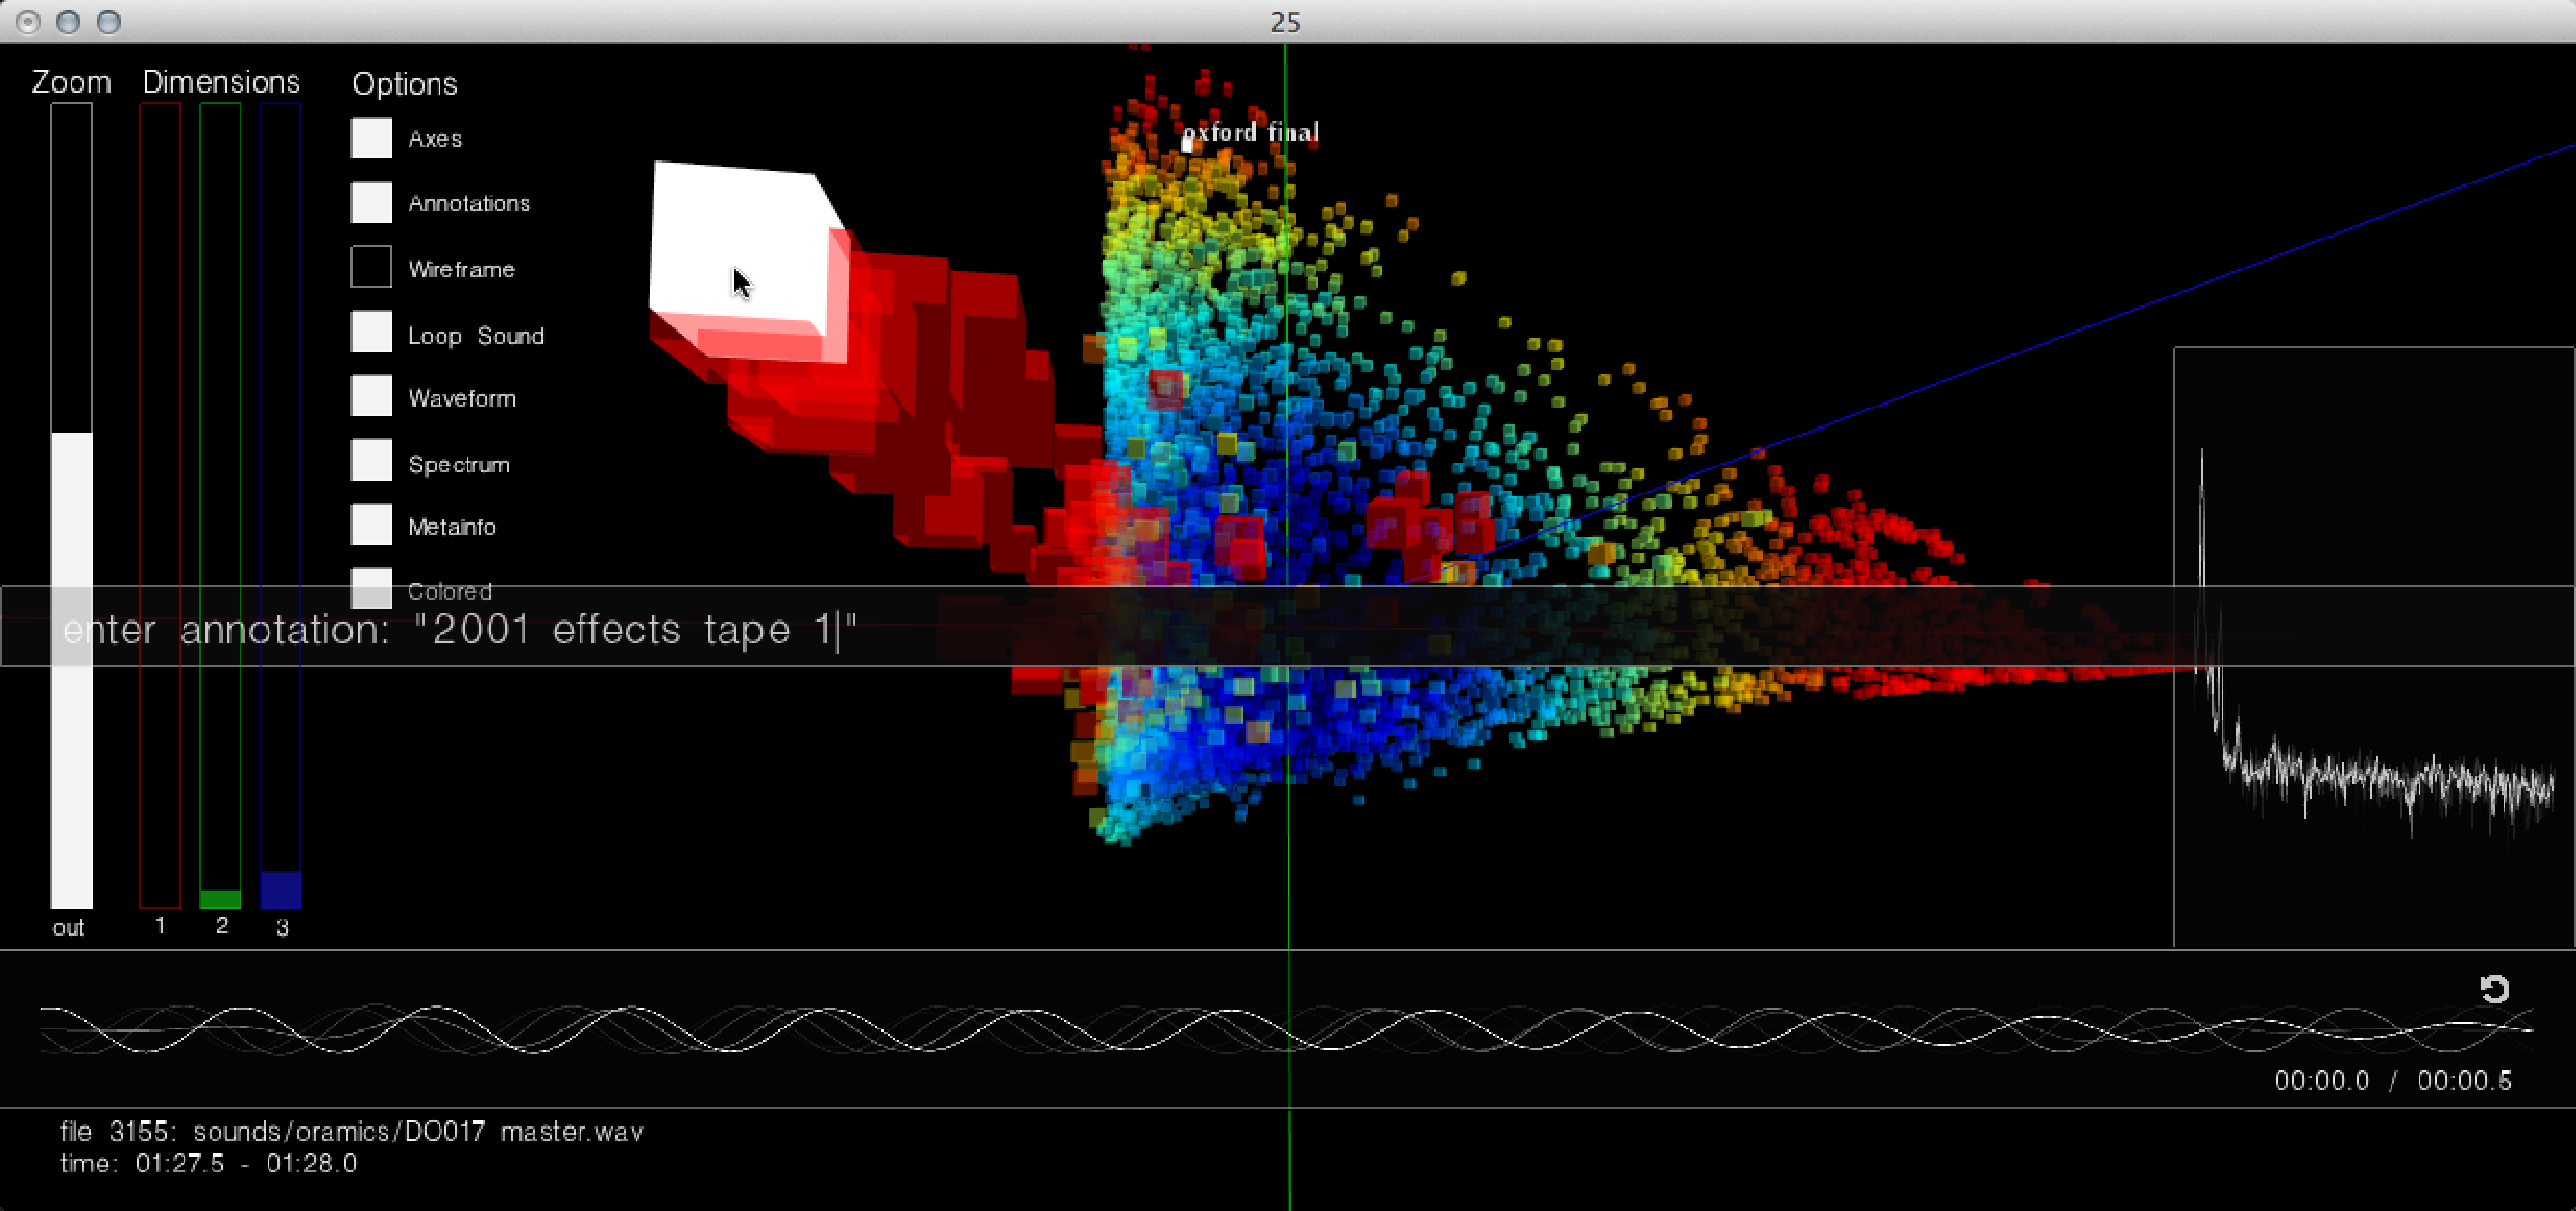
\includegraphics[width=0.99\textwidth]{images/gui.pdf}
  \caption{Screenshot depicting the GUI of the browser (best viewed in color).  Here a user is currently inputing text in order to annotate one of the sound segments.  We can see sliders to the left allowing the user to zoom in/out, change the dimensions of the visualization, and control which elements are drawn on screen.  With all of the options being drawn, we see the waveform of the currently highlighted sound (depicted with a white cube under the mouse cursor) is drawn on the bottom.  As well, the meta-data describing the file name is just below the waveform.  To the right, the decibel-scale spectrum is also drawn.  All elements are drawn in real-time and are interactively manipulated in 3D space.}
\end{figure*}

The interface is shown in Figure \ref{fig:gui} and is built in C/C++ using the creative-coding toolkit openFrameworks\footnote{http://www.openframeworks.cc}.  The user is presented with a 3D space (see Figure \ref{fig:gui}) where each slice of sound from the archive is represented as a cube projected in 3D space.  The coordinates of the cube are determined by which dimensions of the MDS coordinate matrix are selected.  To begin, the first three dimensions are displayed.  Users can then select any dimension to be displayed on the 3-axes.  As a result, the visualization can also be constrained to a 2D visualization by simply choosing the same dimension for 2 axes.  A colormap is used to help depict distance from the OpenGL origin (using a ``jet'' colormap, i.e.: blue-yellow-red), though the user can turn this off.  Figures \ref{fig:plca} and \ref{fig:mfcc} depict the visualizations  of the first three dimensions produced using MDS inside the browser.  

While inside the browser, pressing space-bar allows one to annotate the currently selected slice.  The annotated text appears in 3D next to the slice's cube.  The slice's audio is also visualized as a waveform and its instantaneous Fourier transform.  As we used the first ten minutes of every tape-reel, the waveform for any given slice is presented as a looped region within a 10 minute audio file.  However, the user can change the loop regions to hear any other portion of the original audio file while selecting a slice, thus allowing the user to listen to the audio before and after the slice.

The user can also move the camera around the OpenGL origin by dragging the left mouse button in the 3D space.   Highlighting any of the cubes with the mouse allows the user to inspect the clip in greater detail.  Taking a cue from the 2D analog CataRT, any of the cubes can be ``scrubbed'' for playback by simply moving the mouse over any of the cubes, not requiring any further interaction to listen to the sound sample.  Zooming in and out of the 3D space can be done via the mouse scroll wheel or graphical slider.  Double-clicking on any of the cubes re-centers the origin to the selected cube, allowing camera interaction to occur with respect to the cube.  Cubes can be spaced closer or farther from each other using another graphical slider.  This allows more tightly clustered portions of a visualization to be explored in greater detail.  

%Describe how you derived the PLCA model
%Describe how you derive the MFCC model
%Descirbe the MDS stuff
%Describe how you created the visualisation
%Describe the user studies and how the interface evolved
%State that we worked with the users to make the interface more usable.


\subsubsection{User Feedback}\label{results}

Three researchers of the Oram Archive were invited to navigate the browser and spent 1 hour in total using both the PLCA and MFCC visualizations.  They were unaware of how either model was created, were unfamiliar with signal processing and machine learning, and were only told that we are investigating a way to navigate the Oram Archive.  Each user was given 5-10 minutes of explanation of the features of the browser and were then left to explore the browser by themselves.  Each user proceeded to explore the archive by using the mouse to listen to the different slices located in 3D space.  In addition, each user managed to find particularities of the archive that seemingly would have been very difficult without the browser.  For instance, finding a significant portion of one tape reel that was labeled as ``POP TRY-OUTS'' in another reel labeled as ``COPY DONKEY HELL ABC \& ITV. BIRDS \& PERC'' by exploring slices located near each other in the 3D space.  Also, one found components relating to Daphne Oram's piece, ``Birds of Parallax'' during lectures series that were only labeled by their location, indicating she demonstrated these components during her talk.

When asked to compare the two visualizations and remark on their usability as a navigation tool of the Daphne Oram Archive, the three researchers reported on the form of the MFCC model in comparison to the PLCA one, saying (1), ``it has a less useful shape in general'', (2) ``it has less detail'', and (3) ``this dense mass represents total variety...and I don't quite understand how it is mapped.''  In response, we asked what if anything made the PLCA model more useful for navigation in comparison to the MFCC model.  User 1 reported: ``it has a more definite and understandable space. For example, prongs that have specific information in them such as silence.'' and User 3 reported: ``Oh that's really successful, it seems to be matching pitch and you start to see how she was using pitch'' and ``I had a clear sense of how it was mapped''. 

Each user also gave many helpful possible extensions to the current functionality of the browser, including the ability to save camera states, only view a particular reel's slices, and auto-zoom and rotation around a particular point.  User 1 found the 3D nature of the visualization required more practice saying they ``might get used to it'' while User 3 commented on navigating around a single slice saying ``I understand it as a structure, but I'm working out where in 3D space [the slice] is.  You have to move around in 3D before working it out.''   User 3 also expressed the scope of the browser for new users to see and appreciate Daphne Oram's work, remarking, ``Goes to show just how much variety there are in the samples, and this has made that variety accessible.''  

User 2 additionally remarked on the potential of incorporating other mediums of Daphne's work saying it would be great to ``include other mediums than audio, combining with video/letters/images.''  As well, both User 2 and User 3 commented on the tool's applicability to performance and composition, saying he/she was ``fascinated as a compositional tool.  Navigating different dimensions, it's a beautiful instrument'' and ``it is nice to categorize sounds as it is what we do in sampling''.  

\begin{figure}
  \centering
  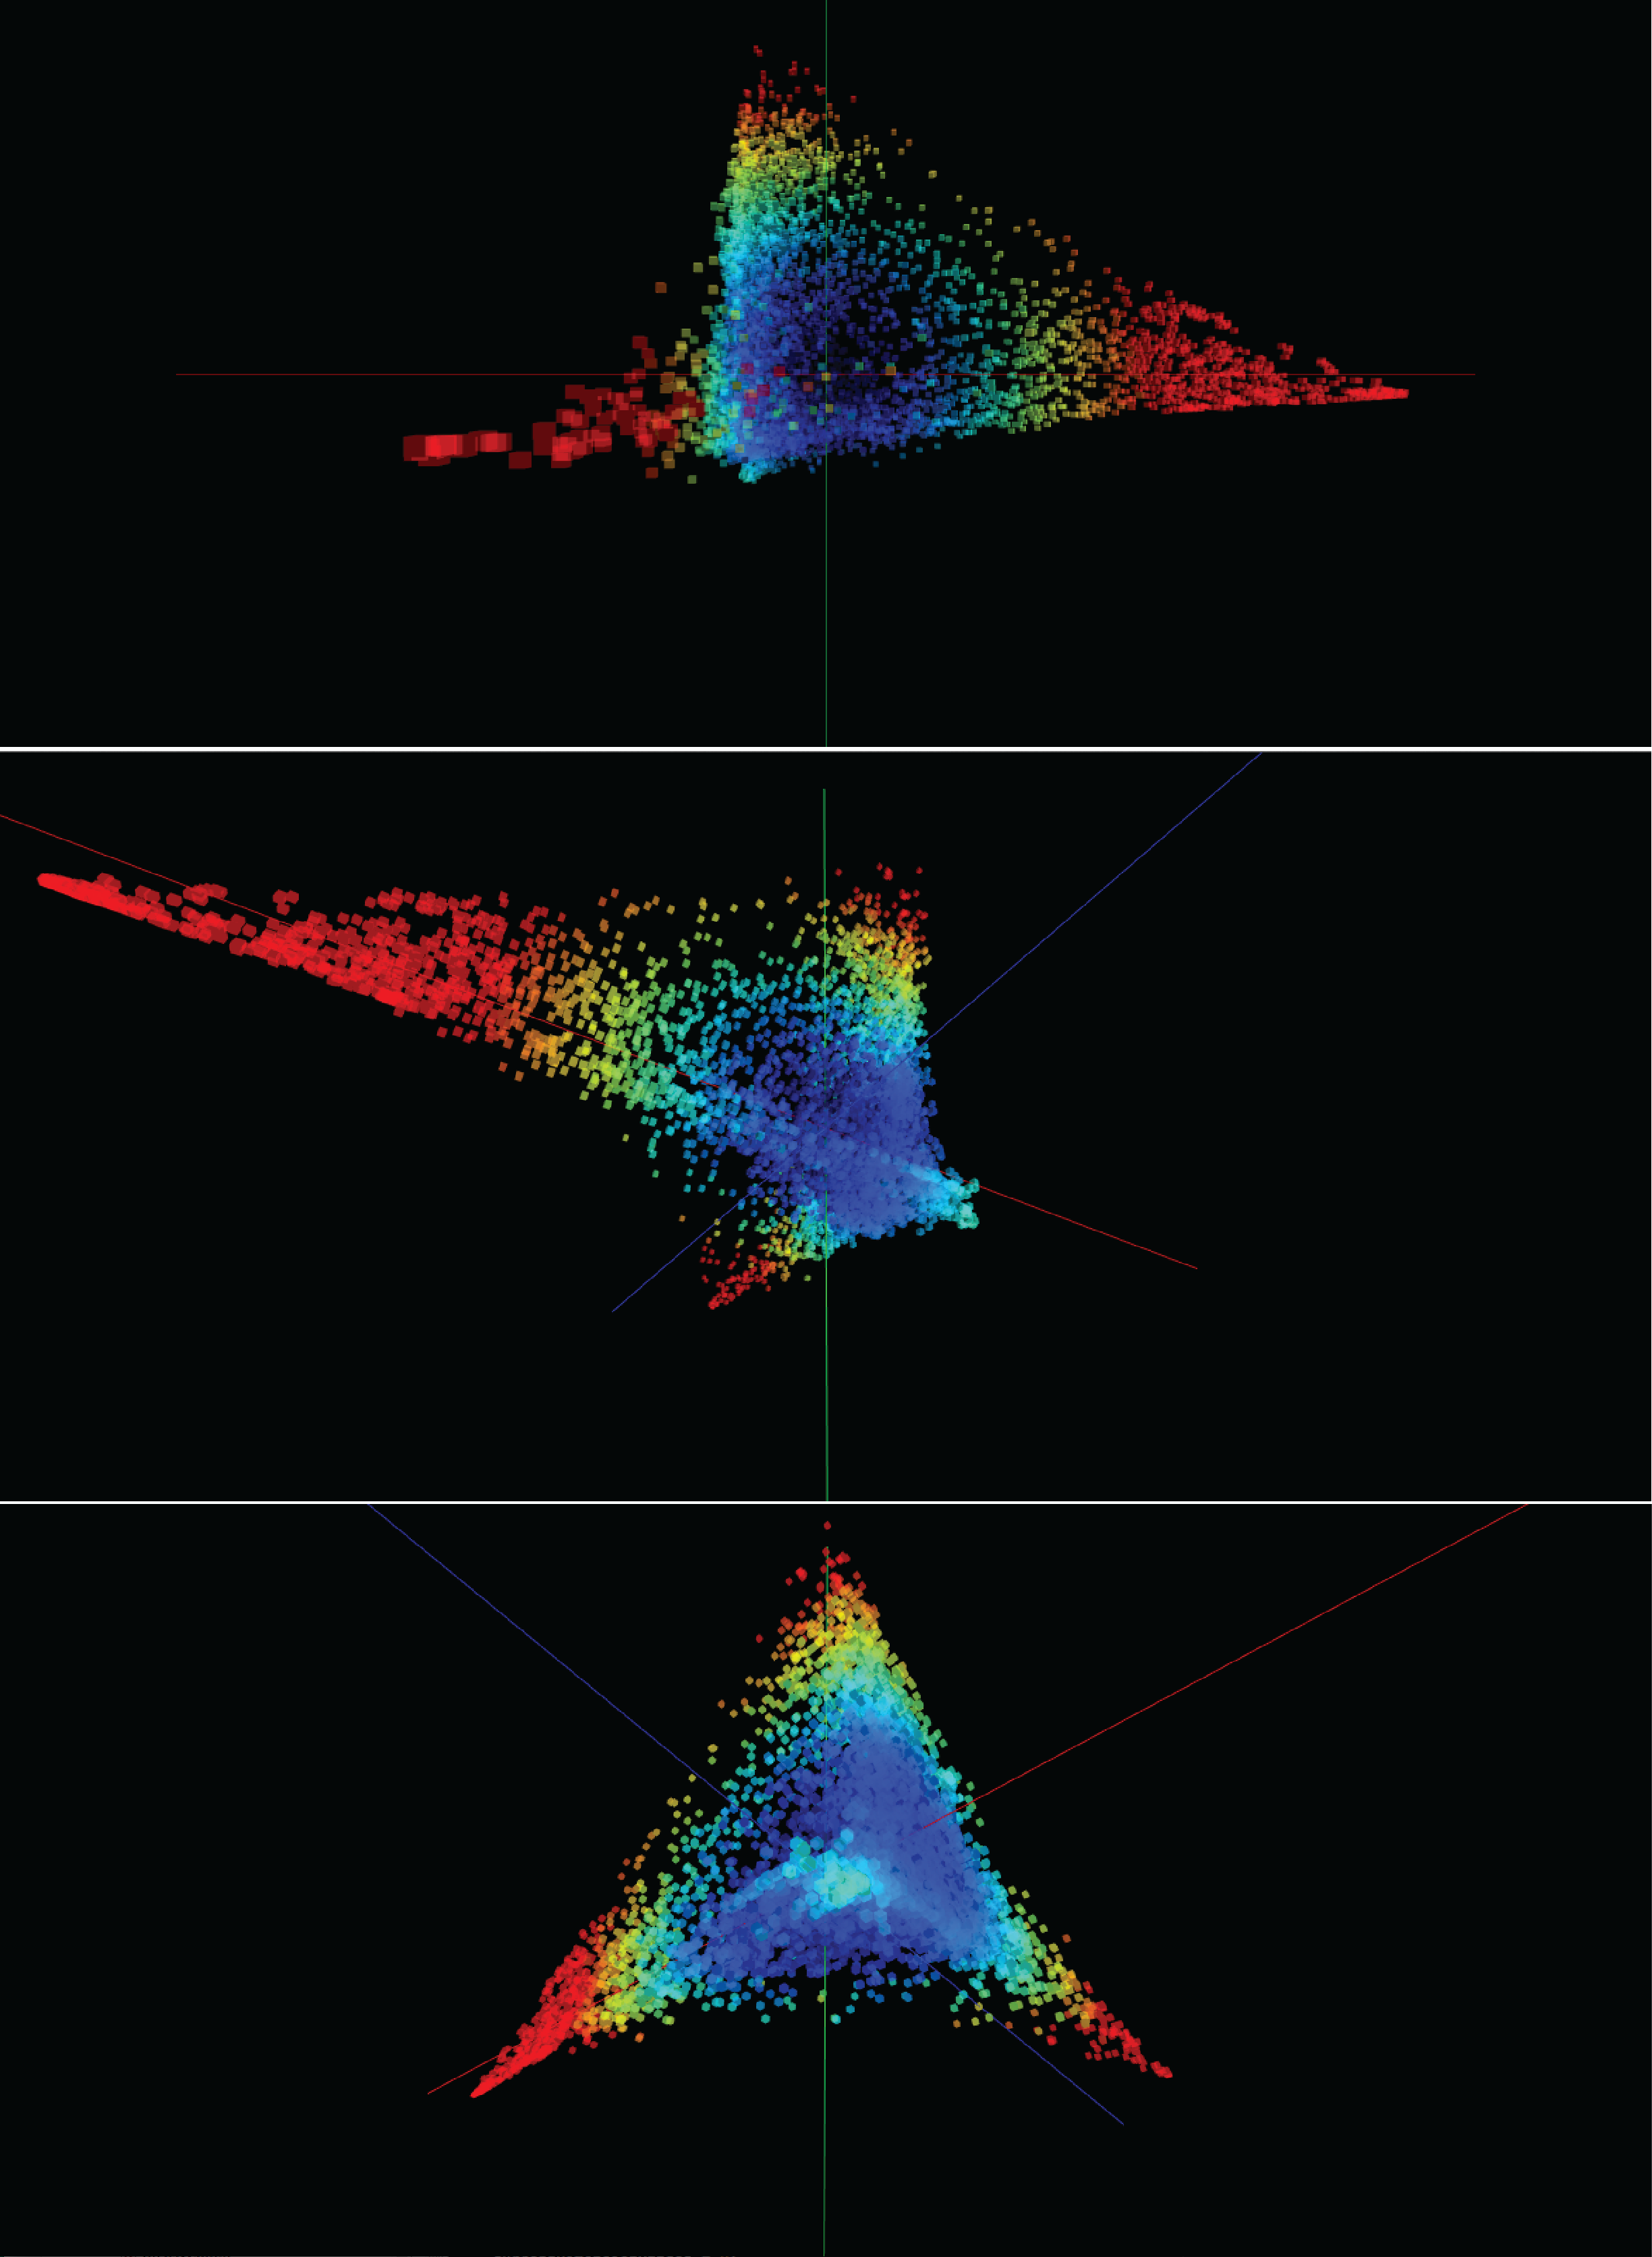
\includegraphics[width=0.38\textwidth]{images/plca-all.png}
  \caption{Screenshot of the first 3 dimensions of the PLCA model visualized in the browser.  We show three different views here.}
  \label{fig:plca}
\end{figure}

\begin{figure}
  \centering
 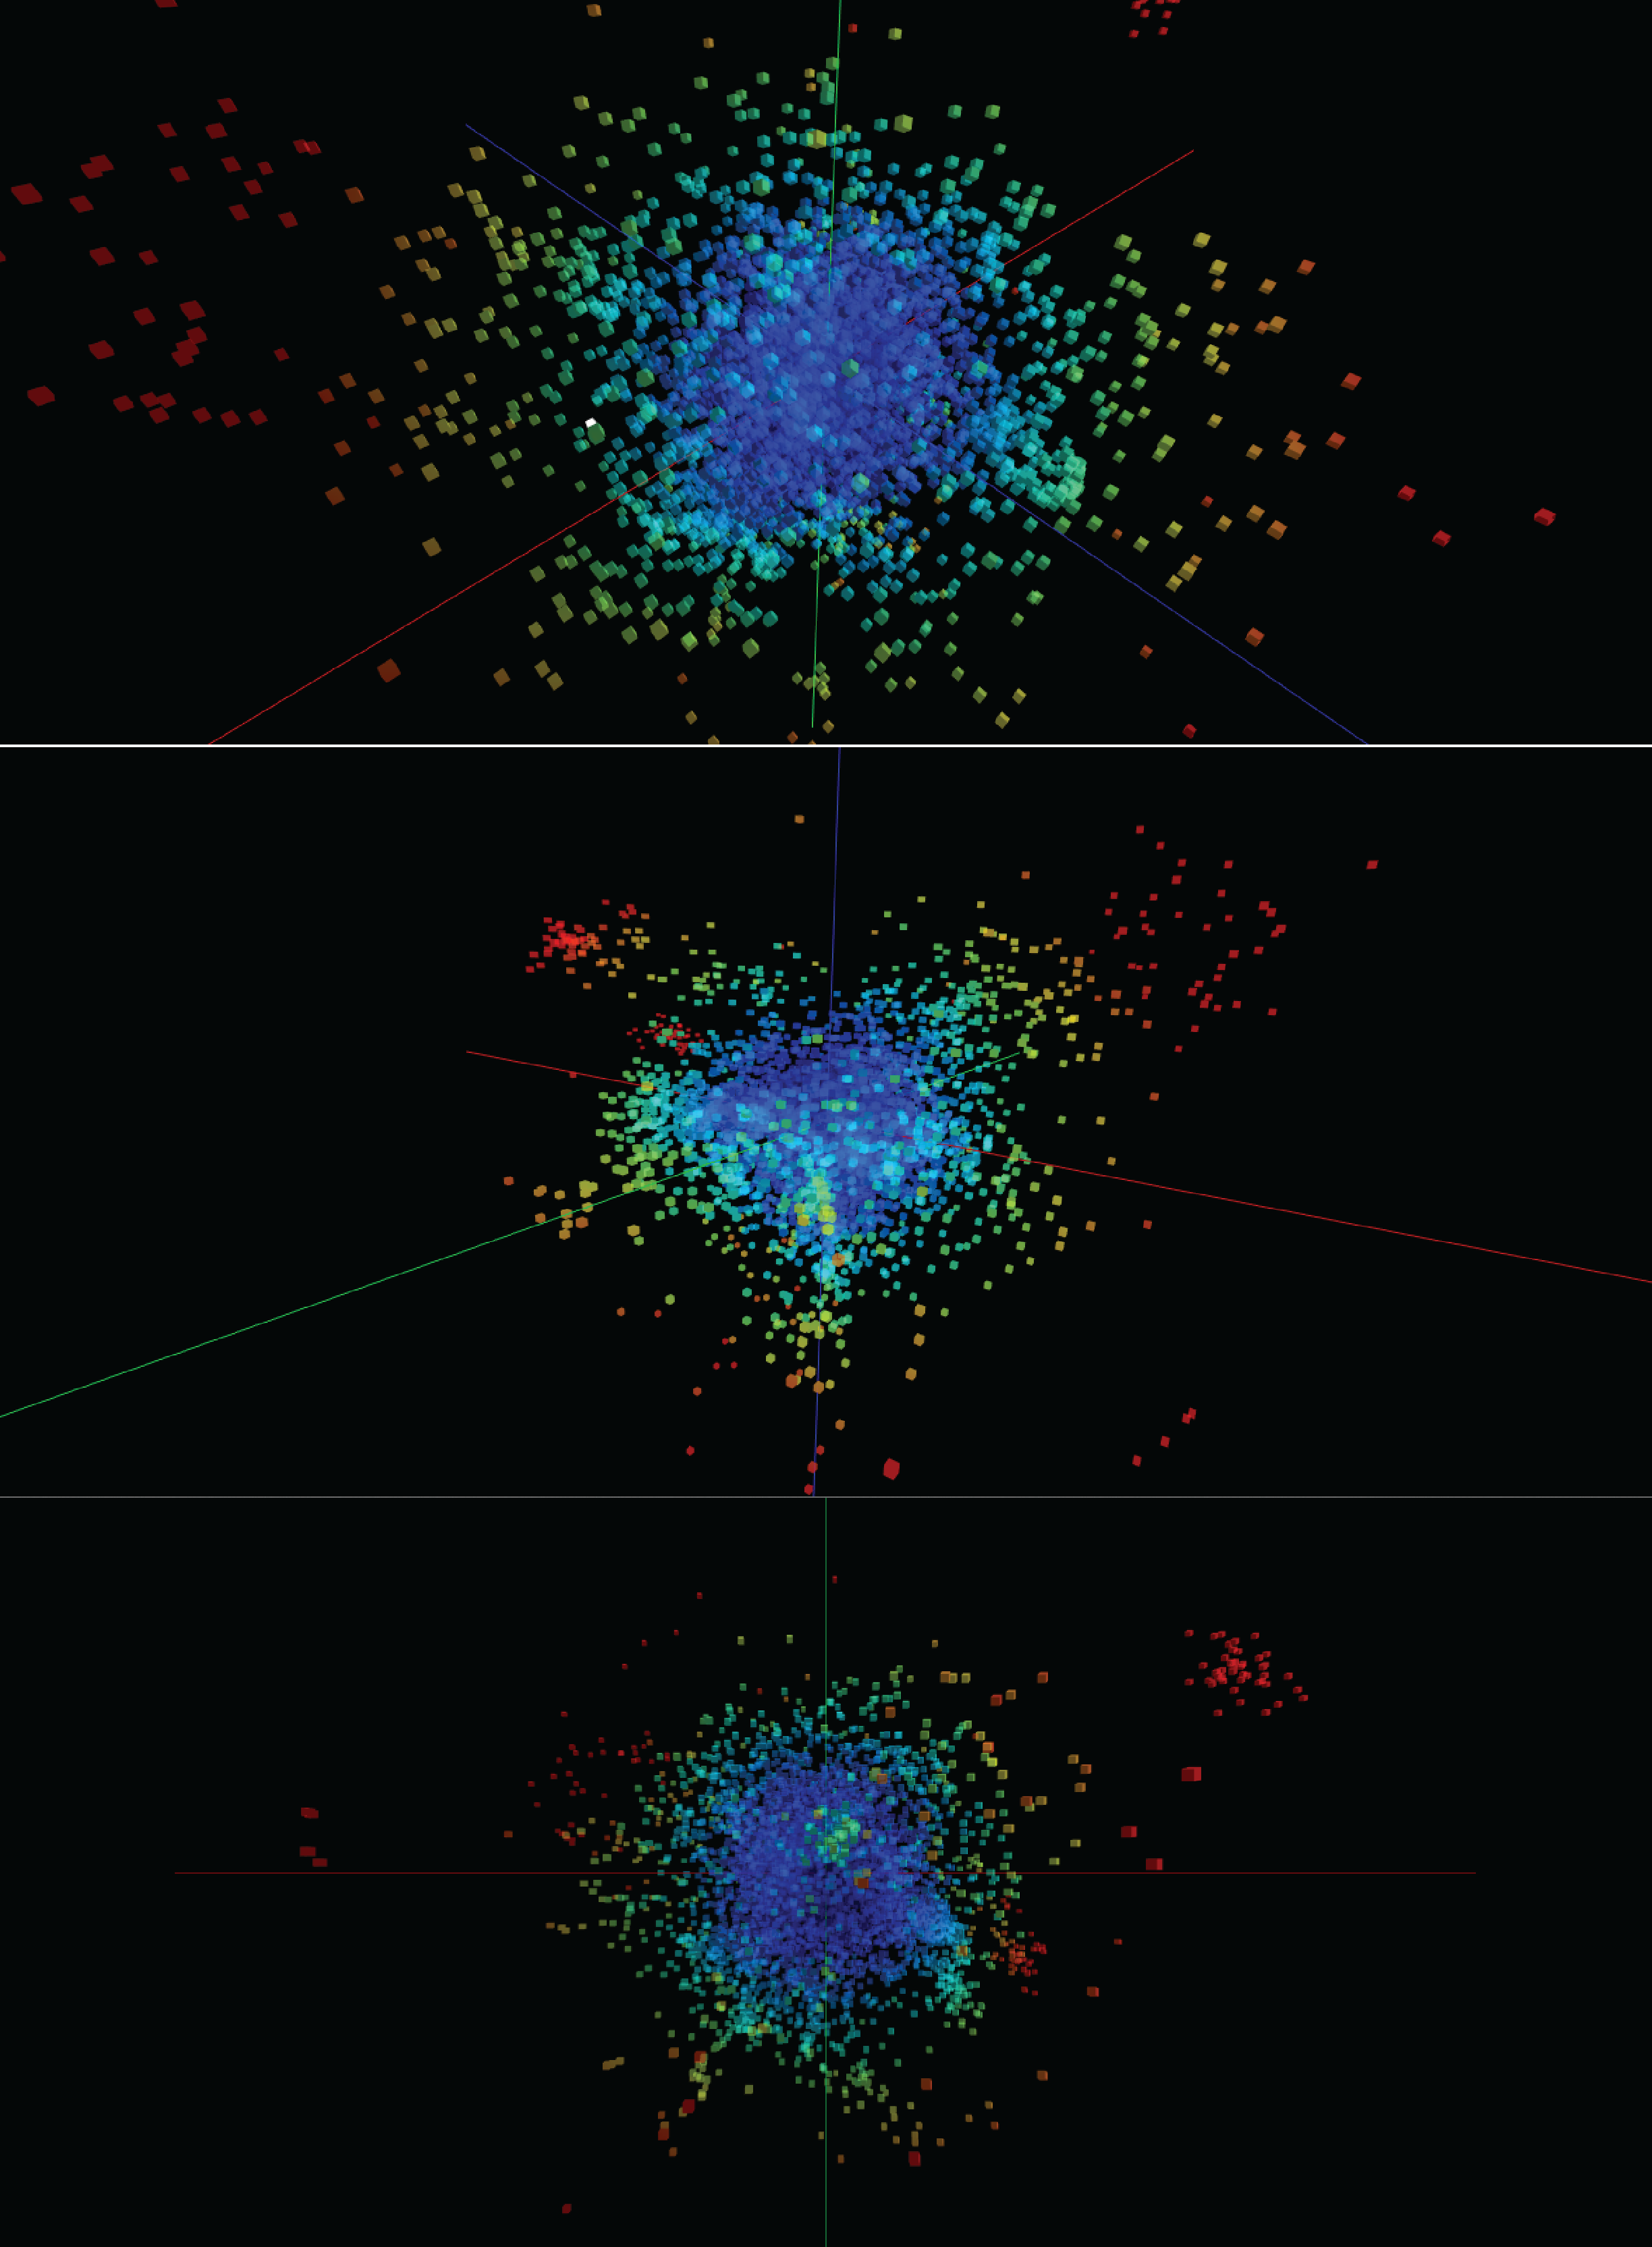
\includegraphics[width=0.38\textwidth]{images/mfcc-all.png}
  \caption{Screenshots of different camera views of the first 3 dimensions of the MFCC model visualized in the browser.  We show three different views here.}
  \label{fig:mfcc}
\end{figure}


%Describe the results of the user studies and how this resulted in changes to the interface.
%Describe that the MFCC model made a far worse visualisation according to the users. DONT discuss why yet.
%Describe how the users responded to those changes
%Detail a few areas where new information was gathered about the recordings.
%Describe how some of our metadata was verified and more clearly understood - we found components relating to Daphne Oram's piece "Birds of Parallax".

\subsubsection{Discussion and Future Work}\label{discussion}

Each researcher had prior knowledge of many aspects of the Archive and Daphne Oram's composition techniques, and were also familiar with many of the recordings.  Their interests in the archive stemmed from her methods in composition to the actual electronics of the Oramics Machine.  When given the chance to navigate the archive in a 3D space arranged by acoustic similarity, each user was incredibly pleased by the possibilities and results of just one hour's navigating, and also preferred the PLCA model to the MFCC one generally for 3 reasons: (1) the visual form and structure of the PLCA model was easier to navigate, as knowing where one was in 3D space is easier to notice, (2), navigating within the ''glob-like'' mass of the MFCC representation in 3D required users to go inside the sphere, making interaction very difficult, and (3), the mapping and clustering in the PLCA model appeared more intuitive, with users reporting they understood how it was mapped and the similarity of sounds along a projection seemed to cluster sounds better.  

Regarding (1) and (2), the form of the PLCA model (see Figure \ref{fig:plca}) is a result of the probabilistic nature of the component weights needing to sum to 1.  In 3D space, this space is defined by a 3-simplex or tetrahedron.  In comparison, MFCCs may have energy explained in all bands as there is no normalization procedure.  Plotting the first three dimensions of the MFCC model thus produces similar distributions of energy in all dimensions, creating what users called both a ``glob like'' and ``blob like'' sphere (see Figure \ref{fig:mfcc}).    Navigating inside and around a sphere presents unique challenges for a 3D browser, namely, it is difficult to select elements within the sphere and understanding the orientation of the sphere is difficult as there are no identifying features.  Thus, exploring visualizations in 3D seems to require landmarks for useful navigation.  In regards to point (3), this may be due to the greater classification and recognition performance of PLCA over MFCCs (left out for blind-review).  

Further work should focus on issues with navigating in 3D space, as some users reported on the 3D nature as requiring practice to navigate.  One solution may be to create more intuitive control through the use of other input and display devices such as touch-screens.  As well, similar latent-analysis techniques may be applied for additional meta-data from the archive as is done in audiovisual and text corpora, e.g. \cite{Himmel1998,Christel1998}, to create more informed visualizations.  In this case, the input of text annotations as well can create a user-guided visualization, where feedback from the user reshapes the 3D visualization. 



\section{Infected Puppets}


\section{Memory Mosaic}


The juxtaposition of fragments of sound as an arts practice has roots at least as early as music concrete, a compositional technique assembling various natural found sounds in order to produce a collage of sound.  Digital Sampling came in the 1970's allowing sound segments to be triggered using an interface such as a keyboard or pad.  More recent techniques have focused on corpus-based concatenative synthesis, where a target sound is matched to a stored database of segments or sounds (for a comprehensive review, see \cite{Schwarz2006}).  Our technical framework most closely resembles SoundSpotter \cite{CaseyICMC2007}, as its framework provides the basis of our auditory feature transformation described in Section \ref{subsec:acoustic-scene-description}.  Though, of the previous techniques mentioned including those in the review article, none investigate corpus-based concatenative synthesis as a real-time experience in an augmented reality.

%Before reaching the culmination of my sound-based practice in ``Memory Mosaic'', an iOS application which automatically creates sound collages based on an aggregation of learned sounds, I will discuss a few practice-based outputs that led me to this application.  
%The first application, ``Sonic Graffiti'', grew out of the desire to create a representation of sonic memories as a spatialized global sonic map.  




%\subsection{Sonic Memory}
%Motivation for implementing an augmented reality which stores ``sonic memories'' and resynthesizes them using the incoming input comes from literature investigating  

\section{Machine Listening Model}
\label{sec:machine-listening-model}

The machine listening model employed in Memory Mosaic is motivated by evidence in  literature of auditory perception stressing the importance of temporal regularities of an acoustic scene in providing continuity for maintaining a cognitive model of an acoustic scene (see \cite{Winkler2009a} for a recent in-depth review).  Such research reinforces Bregman's theory of streaming \cite{Bregman1990}, where one phase consists of the formation of primitive based features, and another on the schema-based selection of streams.  Our model thus places emphasis on temporal discontinuities of the auditory stream using a description of the acoustic scene based on the well-known cepstral coefficients.  % All math operations, including FFT, addition, subtraction, and multiplication are performed using the Apple Accelerate framework in order to achieve real-time performance on an iPhone.  These libraries are made freely available by the authors here: \url{http://github.com/pkmital}.

\subsection{Acoustic Scene Description}
\label{subsec:acoustic-scene-description}

% this needs expanding
Numerous measures of an acoustic scenes have been investigated ...  We make use of one that has the benefit of describing as much of the structure of the acoustic space as possible in order to investigate the regularities at any spectral bandwidth.  

Details of the Log Frequency Cepstral Coefficients (LFCC) feature transformation are described in \cite{CaseyICMC2007}, though is reiterated here for completeness.  The feature transformation begins with the Fast Fourier Transform (FFT) of an audio signal using a fixed frame-size.  For the purposes of real-time augmented reality on the iPhone, at a sample rate of 44100 Hz, a 4096-sample FFT provides high spectral resolution while still being fast enough to perform in real-time.  Following the real-FFT, the magnitudes undergo a Constant-Q Transform (CQT), a real log base-10 operation, and a Discrete Cosine Transform (DCT) in order to produce the 89-element LFCC feature vector.

\subsection{Segmentation Model}

Discontinuity of the spectral shape of an acoustic scene is determined using a statistical model employing the mean and variation of the differences on the distances to a low-pass signal of the features.  The model is described in the Figure \ref{fig:segmentation-model}.  Following the feature transformation, the model has two states of operation: segmenting or not.  When the model is not segmenting, the model of background is built up until a discontinuity appears.  Similarly, for the foreground model, a separate model of the foreground is built up from the start of the segment.  Aside from detecting the discontinuity within the foreground model, the model also detects if the current frame returns to the background model by computing distance to the background model.  Using a prior assumption of a normally distributed feature-space, <<GET A PLOT OF A BUSY STATION'S DISTRIBUTION OF FEATURE VALUES>> we compute deviations of the background and foreground model past 3 standard deviations.  As well, checking whether the currently observed audio frame returns to background, we check if its features are within 3 standard deviations of the background model and stop segmenting.  A parameter controlling the threshold of the standard deviation, between 0.1 and 3.0 standard deviations, is described in Section \ref{subsec:parameters}.

Each new segment detected is written to disk using Apple's Extended Audio File Format.  Only the audio segment's first frame's 89-dimensional LFCC feature vector is retained in memory in order to form a matrix of vectors.  As our model is based on attentional shifts,

% uhh...

\section{Concatenative Synthesis Engine}

The concatenative synthesis engine describes any input sound using a polyphonic reconstruction from its database of sound segments.  At each new onset determined by a temporal irregularity of the acoustic scene, a new set of matches are constructed to the current audio frame.  The onset detection for the synthesis engine is much like the one for the segmentation model; however, no foreground model is kept, and only the background model may deviate, creating new background models at each onset.  Thus, the model does not require knowing what is foreground or background, and only requires deviations in the continuous acoustic space.  

% include graphic of the algorithm here.  

\subsection{Matching}

Matching can be formulated as a nearest neighbor algorithm which begins by creating a metric space $X$ of known points $P = p_1, p_2, ..., p_n$ for $n$ points.  These points are pre-processed in such a way that a neighbors to any query point, $q \in X$, are found quickly.  To pre-process the points, we use a distance metric to keep the 3 highest matches to any query point using a simple linear index.  Iterating linearly over the dataset of LFCC vectors, the 3 best matched vectors' indices are kept using cosine similarity, which measures the angle between two vectors $A$ and $B$ like so:

\begin{math}
\textnormal{similarity} = \cos(\theta) = {A \cdot B \over |A| |B|} = \frac{ \sum\limits_{i=1}^{n}{A_i \times B_i} }{ \\ \sqrt{\sum\limits_{i=1}^{n}{(A_i)^2}} \times \sqrt{\sum\limits_{i=1}^{n}{(B_i)^2}}} 
\end{math}

Using Apple's Accelerate framework, this metric can be computed using efficient vector operations that are optimized for the iPhone:
\clearpage
\begin{program}
\begin{verbatim}
float cosineDistance(float *x, float *y, unsigned int length) {
	float dotProd, magX, magY;
	float *tmp = (float*)malloc(count * sizeof(float));
	
	vDSP\_dotpr(x, 1, y, 1, &dotProd, length);
	
	vDSP\_vsq(x, 1, tmp, 1, length);
	vDSP\_sve(tmp, 1, &magX, length);
	magX = sqrt(magX);
	
	vDSP\_vsq(y, 1, tmp, 1, length);
	vDSP\_sve(tmp, 1, &magY, length);
	magY = sqrt(magY);
	
	delete tmp;
	
	return 1.0 - (dotProd / (magX * magY));
}
\end{verbatim}
\caption{Vectorized code for performing cosine distance}
\end{program}

\section{Application}

\subsection{Parameters}
\label{subsec:parameters}

\section{Discussion}

John Oswald; Burrough's Cut-up-technique; Scrambled Hackz; Collins; Casey; Grierson; Schwarz...


%%%%%%%%%%%%%%%%%%%%%%%%%%%%%%%%%%%%%%%%%%%%%%%%%%%
%%%%%%%%%%%%%%%%%%%%%%%%%%%%%%%%%%%%%%%%%%%%%%%%%%%
%%%%%%%%%%%%%%%%%%%%%%%%%%%%%%%%%%%%%%%%%%%%%%%%%%%
%%%%%%%%%%%%%%%%%%%%%%%%%%%%%%%%%%%%%%%%%%%%%%%%%%%
%%%%%%%%%%%%%%%%%%%%%%%%%%%%%%%%%%%%%%%%%%%%%%%%%%%
%%%%%%%%%%%%%%%%%%%%%%%%%%%%%%%%%%%%%%%%%%%%%%%%%%%
%%%%%%%%%%%%%%%%%%%%%%%%%%%%%%%%%%%%%%%%%%%%%%%%%%%



%%%%%%%%%%%%%%%%%%%%%%%%%%%%%%%%%%%%%%%%%%%%%%%%%%%
%%%%%%%%%%%%%%%%%%%%%%%%%%%%%%%%%%%%%%%%%%%%%%%%%%%
%%%%%%%%%%%%%%%%%%%%%%%%%%%%%%%%%%%%%%%%%%%%%%%%%%%
%%%%%%%%%%%%%%%%%%%%%%%%%%%%%%%%%%%%%%%%%%%%%%%%%%%
%%%%%%%%%%%%%%%%%%%%%%%%%%%%%%%%%%%%%%%%%%%%%%%%%%%
%%%%%%%%%%%%%%%%%%%%%%%%%%%%%%%%%%%%%%%%%%%%%%%%%%%
%%%%%%%%%%%%%%%%%%%%%%%%%%%%%%%%%%%%%%%%%%%%%%%%%%%





\chapter{Conceptual Framework for Building Unconscious Visual Representations}
\label{ch:conceptual-visual}
\minitoc

\section{Introduction}

The world in front of us is measured by the various sensory mechanisms we have available to us: eyes, ears, fingers, etc... These mechanisms enable us to convert the physical phenomena into electrical signals that we use to construct a perception of the world.  However, we are often taught that the world we see is exactly as it is in front of us.  Philosopher Alan Watt's describes this predicament:
\begin{quotationb}
Most of us are brought up to feel that what we see out in front of us is something that lies beyond our eyes, out there. That the colors and the shapes that you see in this room are out there. In fact, that is not so. In fact, all that you see is a state of affairs inside your head. All these colors, all these lights, are conditions of the optical nervous system. There are, outside the eyes, quanta, electronic phenomena, vibrations, but these are not light, they are not colors until they are translated into states of the human nervous system. So if you want to know how the inside of your head feels, open your eyes and look. That is how the inside of your head feels\\
\flushright{\textsc{Alan Watts}}
\end{quotationb}
How it feels at certain levels...what these representations look like... build up theory... 


William Gibson

J. J. Gibson

... 

\section{Background}

In a seminal study on visual perception published in 1921, Rubin describes a fundamental form of experience consisting of a figure standing on a ground.  The figure describes the focal or fundamental experience of a scene, whereas the ground describes the ambient or marginal portions of a scene.  Expanding this point further in the 1920's, the Gestalt psychologists developed a comprehensive perceptual theory employing figure-ground as a fundamental type of perception where the notion of a Gestalt, or totality, is described by a figure and ground.  The Gestalt describes the fundamental experience of perception.  As a result, any subdivision or interrogation of a part of the Gestalt would alter experience into yet another figure and ground relationship \cite{Wever1927}.  

From these seminal studies, visual perception research has continued in trying to understand how the brain supports the formation and understanding of such figures.  The physiology and behavior of the eye has given researchers in visual attention and active visual cognition a unique window into the brain.  Starting with the physical wavelengths of light entering our eyes, we rapidly shift our gaze an average of 3-5 times a second, completely disrupting the continuity of light entering our eyes.  Visual acuity limitations mean that our eyes require rapid ballistic movements of the eye taking all of 30 ms (a \textit{saccade}) to project the light from the particular point of a visual scene we are interested in onto a 2-degree area of the retina with the highest spatial resolution (the \textit{fovea}).  Going away from the fovea (the \textit{parafovea}), resolution for spatial detail drops logarithmically, while resolution for motion detail increases, a relationship due to the distribution of photo-receptive cells in the eye combined with the lens of the eye itself.  

As our parafovea has been engineered for high motion resolution rather than high spatial resolution, we cannot encode with high spatial detail an entire visual scene at once, as a camera with a small aperture may be able to do.  Instead, we require an active viewing of a scene in order to perceive the details of a scene.  We do this through the use of saccades and head-movements to move and finally stabilize (a \textit{fixation}) our eyes to the region of interest, a process lasting on average 330 ms.  During this time, it is thought that the encoding of details at the point of fixation into memory occurs as well as planning of the next eye-movement \cite{}.  

\subsection{Attention}

The focus of research in eye-movement behavior has investigated why, where, and in which circumstances we move our eyes.  The earliest studies \cite{Buswell1935,Yarbus1967} describe two main influences of a viewer's attention to a visual scene: (1) influences dependent on mental states which focus attention towards contextually and cognitively relevant aspects of the world (\textit{endogenous}), and (2) influences dependent on involuntary capture of attention from the external environment (\textit{exogenous}).  As exogenous factors are involuntary, one would expect to find the behavior influenced by these factors to be highly consistent across viewers.  In contrast, as endogenous influences are dependent on cognitive factors resulting from emotion, memory, language, task, and previous experiences, the relation of a scene and one's endogenous influences on the scene are much less consistent across viewers.  

\subsubsection{Exogenous Influences on Attention}

In seminal work investigating the speed of visual perception using Gestalt primitives, Sziklai demonstrated the human visual system exhibits an attentional bottleneck of 40 bits per second on selected information, suggesting our visual systems require a simplified representation from the many megabytes per second of information coming from exogenous visual information \cite{Sziklai1956,Merrill1968}.  Much research investigating exogenous influences on static visual scenes therefore describe a simplified representation of attentional control known as a \textit{bottom-up} model \cite{Koch1985,Itti1998,Wolfe1989,Itti2001}.  Such models are built around theories of feature-integration \cite{Treisman1980} and are further supported by physiological evidence of the receptive fields and visual architecture of the visual cortex of cats \cite{Hubel1962}.  To discover the attentional biases for portions of a scene (\textit{saliency}), bottom-up models recompose a full resolution image using filter banks tuned to multiple frequency orientations and scales corresponding to pre-attentive visual features also found in early visual cortex such as luminance, oriented edges, and color contrasts.  Saliency is then computed as a weighted linear summation (\textit{integration}) of the resulting ``feature maps'' formed of different scales. 

It is thought that basic feature levels of models of integration are modulated by what Itti et. al calls ''top-down'' influences \cite{Itti2001} such as the current ongoing task \cite{Yarbus1967,Smith2011a} and the context of a scene in order to reduce processing load \cite{Henderson2003,Torralba2006}.  Though, the level at which top-down influences may affect processing is still open to debate.  Further, though these modulations are often described as top-down influences, such a term should not be confused with endogenous influences, as much research has shown that memory, context, and other endogenous factors affect early visual processing \cite{Tatler2011} which would correlate with initial feature stages thought to be unaffected in a bottom-up model.  Further, gist-based models (presented later) separating ``conceptual'' and ``perceptual'' influences may similarly be looked at in terms of ``bottom-up'' and ``top-down'' influences, or even ``exogenous'' and ``endogenous''.  As a result, these terms all vary slightly in their use and meaning, which should be no surprise given the complicated nature of the brain.  For the purposes of this thesis, endogenous and exogenous seem to offer the most useful definition separating influences originating from the brain and from the sensorial world, respectively, and other distinctions, e.g. bottom-up/top-down, are not used. 

Clustering of gaze during dynamic scene viewing -> motivate flicker as an attentional map, prior to understanding temporal incoherences, sets basis for proto-object representation later... discuss attentional synchrony paradigm... 
  	
\subsubsection{Endogenous Influences on Attention}
\label{sec:endogenous-influences}

In a seminal study on how task affects eye-movements during static scene viewing, \cite{Yarbus1967} tracked the eye-movements of participants viewing a painting entitled, ``An Unexpected Visitor.''  His study showed that when participants viewed the painting and were given a task such as to determine the ages of the people in the painting, they looked more at the faces of each person.  When asked to determine what they were wearing, their eye-movements strayed away from faces, and looked more towards the clothing of people.  Yarbus further describes 7 different tasks and shows how the eye-movements of each participant reflects the information required for processing the task at hand.  It is thought that task, therefore, is an endogenous influence.

In a similar study on dynamic scene viewing, Smith studied task-based effects on viewers' eye-movements looking at unedited videos of natural scenes from a camera mounted on a tripod \cite{Smith2011a}.  Participants were natives to the city of Edinburgh and viewed a variety of indoor and outdoor scenes from the city.  The study revealed that during free-viewing, i.e. not given any task other than to look at the video, participants looked at mostly moving objects such as people moving across the frame or cars.  However, when given the task to identify the location of the presented scene, participants had to concentrate their gaze towards the elements of a scene depicting landmarks such as buildings, signs, and trees and showed a remarkable ability to distract away from moving objects.  After viewers pressed a button indicating recognition of the location, their viewing behavior reverted to resembling the free-viewing task, fixating on moving objects such as people and cars again.  The study re-asserts the findings of Yarbus, though for a dynamic time-course.  Further, it also provides evidence of default viewing conditions during the time-course of viewing, as participants were able to ``return'' to the free-viewing task after having finished the task of recognizing the location of the scene.  

Discuss use of attentional synchrony paradigm in smith paper and in Melissa's paper too...

\subsection{Gist}
\label{sec:gist}

<<Introduce RSVP. then introduce gist more before saying what its findings entail... >>

The ability to classify scenes with rapid pre-attentive processing lasting only 45-135 ms (\textit{Gist}) \cite{Potter1969,Biederman1974,Potter1976,Schyns1994,Henderson1999} suggests that the general shape and structure of a scene leading one to infer its context are defined by either volumetric forms (\textit{geons}) \cite{Biederman1987}, spatial arrangement of blobs defined by contrasts in luminance or color \cite{Schyns1994,Oliva1997} or by using a scene's spatial frequency content \cite{Oliva2001,Oliva2005}.  A scene's spatial frequency content can be described by oriented band-pass filters: at a low spatial frequency, this content resembles broad edges and the layout and orientations of a scene's largest similarly textured regions, whereas at a high-spatial frequency, the response of the sharpest edges and their directions are encoded.  

Endogenous influences on subsequent processing of gist seem to influence the spectral scale at which gist is selected \cite{Schyns1994,Oliva1997}.  Schyns and Oliva describe an experiment where a low-spatial frequency (\textit{LSF}) and a high spatial frequency (\textit{HSF}) image are created for two separate pairs of images.  Creating two new images by combining the LSF of one image and the HSF of the other, and vice-versa, they investigate the scale space of gist recognition with and without a verbal cue to indicate what type of scene will follow (\textit{priming}).  Without priming, subjects are able to recognize the scene described by the LSF content of an image given 45 ms of presentation time, and the HSF one within 135 ms.  As well, subjects are unaware of the content in the other scale space (i.e. shown an image with LSF and HSF content for 45 ms, the participants are unaware of there being separate HSF content).  However, being primed with either the LSF or HSF content of the scene, subjects report perceiving the given cue instead.  

While gist is thought to be pre-attentive, i.e. before the timescale of acts of selective attention, such research suggests either that (1) the scale at which the early representation of gist operates at is affected by task-demands (i.e. only one scale of gist is encoded for pre-attentively), or (2), attention and further encoding into memory is dependent on endogenous influences on scale selection, (i.e. gist may be encoded at multiple scales, but only the scale selected by attentional machinery is encoded into memory).  Though not all scales are necessary for determining a scene's content when given prior cues (\textit{priming}), the neurobiology of early visual cortex gives scope for encoding of multiple visual scales.  It thus seems possible to assume (2) is a more likely model for the interaction of gist and attentional machinery.

<<Talk about features diagnostic to a scene's description, and how they accelerate or impair recognition of a scene, e.g. color in natural environments (Oliva, 2005).>>

Oliva further argues for two types of gist, \textit{conceptual} and \textit{perceptual}.  Conceptual gist refers to semantic information inferred from viewing a scene or from shortly after a scene disappears. Perceptual gist is thought to be motivated by the given task at hand in order to provide the structure or form of a scene and uses pre-attentive low-level information such as color, orientation, depth, and motion (Oliva, 2005).  <<Need to explain these much more as they go back into proto-objects and should be related to endo/exo as well etc...>>
	
Gist has been understood in terms of the classic rapid serial visual paradigm (RSVP), or within a screen based presentation where stimulus presentations are preceded by empty or noisy screens.  However, the real-world is not preceded by such screens, and rather the notion of gist across saccades, in a situated world becomes an important one to make.  How does a dynamic model of gist help us to maintain a coherent perspective of the world, and further guide our attention?  

\subsection{Change and Inattentional Blindness}

Research demonstrating the failure to report large changes in the visual world (\textit{change blindness}) as well as the failure to report unexpected visible changes due to task requiring attention elsewhere (\textit{inattentional blindness}) \cite{Simons1999,Rensink2000,Rensink2001,Hollingworth2001a} have shown that our visual systems are unaware of changes in visual world outside of the point of fixation.  Simons and Chabris demonstrated '\textit{Inattentional Blindness} by composing a video of two basketball teams dressed in white and black passing a ball to each other \cite{Simons1999}.  Participants were asked to count the number of passes that the white team makes.  During the course of the video, a person wearing a gorilla suit walks across the frame of the camera, unnoticed by 75\% of participants.  The phenomena of \textit{Change Blindness} was demonstrated in a real-world psychology experiment \cite{Simons1998} where participants arrived at a kiosk to fill in a consent form and hand the completed form to a man behind the counter.  The man ducks behind the counter as to pretend to file the paper, while a different man comes up from behind the counter, again unnoticed by a majority of the participants.  

Failing to detect changes outside of the point of fixation suggests that any peripheral representation of a scene would likely not encode details of object specific features such as color, motion, or orientation gratings.  Rather, our visual machinery integrates the detailed aspects of objects across eye-movements, retaining that information as a perceived representation of the visual world.  The broad spatial scale afforded by the lens of the eye and the higher motion resolution afforded by the spacing of cones in the periphery give further indication to the lack of highly detailed feature encoding in the periphery.  Though, to what form, and to what detail a periphery representation may encode is still an open question.  

Rensink takes this evidence in developing a theory of coherence, proposing that object representation depends on focal attention.  For objects outside of the point of fixation, Rensink proposes we encode volatile units of \textit{proto-objects} \cite{Rensink2000,Rensink2001}.  Proto-objects are argued to be amorphous and blob-like in nature, representational-less and concept-less lasting only a few hundred milliseconds.  It is further argued that attention operates on groupings of proto-objects rather than at the earlier feature levels making it the highest level of early vision, and the earliest operands of selective attention.  Rensink also hypothesizes that proto-objects may explain non-attentive processes capable of recognizing the abstract meaning of a scene and the spatial layout of the scene \cite{Rensink2002}.  In relation to perceptual influences, implicit behavioral measures suggest that grouping processes can also occur for task-irrelevant visual stimuli, i.e., for stimuli that has not been attended to by a fixation, further supporting theories of proto-object formation \cite{Lamy2006}.

%\subsection{Electrophysiology}\label{sec:electrophysiology}
%Visual Mismatch Negativity... reviews in Czigler 2007, 2010...
%\cite{Stefanics2011}
%Border-ownership in V2 modeled by lateral interactions, producing self-organizing structures resembling shapes.
%Violation of sequential rules elicited for a deviant color (Czigler 2002), orientation (Kimura 2010), movement (Pazo-Alvarez 2004), spatial frequency (Heslenfeld 2003), contrast (Stagg 2004), sequential conditional relationships (Stefanics, 2011), and even facial expressions (Zhao and Li, 2006)
%Marr, invariances...

\section{Conceptual Framework}

\subsection{Visual Acuity}

Models function of the eye to develop higher spatial acuity at fixation... Higher motion resolution outside of fixation.

\subsection{Exogenous Attention Model}

Flicker, motion cues.

\subsection{Proto-objects}

Spatial grouping of color, motion, and luminance cues.  Builds a shape representation.

\section{Discussion}

Research in change blindness has indicated that though we experience a rich, detailed visual world, we do not use such rich details in building a stable representation \cite{Simons1997}.  Rensink argues that object representation requires focal attention.  However, in considering an architecture of visual perception, what is the cause of producing focal attention?  The literature presented here suggests that there is either an endogenous explanation or exogenous one.  For example, I may focus on a cup, but not build the representation of the fingerprints on the cups as I was not intending to look at this particular scale.  In this case, the endogenous influence of perceiving the object representation of fingerprints on the cup was necessary for building such a representation, even though focal attention will have brought my eyes to the cup.  It may be that my task of drinking from the cup saw the cup as what it afforded: a drink.  In a free-viewing task, if such a thing exists, it may be more likely that an exogenous influence such as the mis-representation of the cup will provoke more detailed representations and cause additional focal attention to the cup.  Thus, it may be the case that focal attention is necessary for explaining an object, however, it seems it is not sufficient and the cause of focal attention should still be considered.  

When considering evidence for gist in relation to Rensink's theory of coherence, it seems viable to consider proto-objects as the same representation that gist may use \cite{Rensink2002}.  Though Schyns and Oliva argue for using oriented banded filters, it is not unlikely that collections of blob-like entities which necessarily also respond to the scale of the proto-object could provide a cue for spatial layout.   However, when considering evidence in rapid determination of the meaning of scenes, Schyns and Oliva demonstrated that early processing of a scene could be re-organized based on prior experiences \cite{Schyns1994,Oliva1997}.  Thus, it is not clear from their research alone whether the pre-conceptual representation itself can be changed, or if only the attentional machinery acting on a set of possible representations has changed.  The latter effect would entail a sort of conceptual prior on a scene, suggesting the organization of a scenes early representation remains untouched.

Pylyshyn theorizes that the understanding of a concept is not all that is required for visual experience: 
\begin{quotationb}
''Vision suited for the control of action will have to provide something more than a system that constructs a conceptual representation from visual stimuli; it will also need to provide a special kind of direct (preconceptual, unmediated) connection between elements of a visual representation and certain elements in the world. Like natural language demonstratives (such as 'this' or 'that') this direct connection allows entities to be referred to without being categorized or conceptualized. \cite{Pylyshyn2001}''
\end{quotationb}  
The preconceptual connections Pylyshyn describes are easily described by the pre-attentive proto-objects Rensink also describes \cite{Rensink2000,Rensink2001}.  What is interesting in Pylyshyn's theory is the notion that this pre-conceptual representation does not need to be categorized or conceptualized in order to be referred to.  In other words, the categorization which Pylyshyn theorizes of is part of the attentional machinery which refers to proto-objects, rather than an explicit property of the proto-object themselves.  According to Pylyshyn's theory, proto-objects of a visual scene are then described by one particular fate, and attentional mechanisms can only select from the set of possible proto-objects, rather than influence their definition. 

Proto-objects act as an indexical reference to a conceptual referent.  How proto-objects are defined is based on the features that best give coherence to the scene.  They are also scaled with increasing eccentricity, presumably at least because of the shape of the eye would decrease spatial resolution, but as well due to the nature of attention acting at the point of fixation.  Functionally, visual material outside of the region is of less importance to the task at hand.  Thus, the biological nature of the shape of the eye could also be understood in terms of evolving to act in the world.  Proto-objects may also possibly find re-definition from the act of attention.  As proto-objects are volatile in nature, the act of attention reshapes ones perspective of a scene, thus reorganizing the boundaries defining proto-objects, even at the point of attention.

Global shape as in the gist of a scene gives a context for defining the possible scale of proto-objects.  As well, the collection of proto-objects themselves can be understood as a scene's shape.  In audition, the shape could be defined as the timbre, or what frequencies the sprectrum may generalize to, as in MFCC or LFCC features.  Proto-objects for audition may be thought of in terms of independent components in a matrix factorization of a time-frequency matrix.  These components map to gestalts of spectral information.  They are also understood in the Bregman sense of streams as they are perceptual units that are also volatile depending on the current auditory information and perception of the viewer.

\section{Conclusion}

Needs a rewrite.

Considering both the implicit, unmediated representation and the attentional and contextual mechanisms, at least two critical layers should be built into any computational model based on the evidence presented here:  (1), a pre-conceptual representation which takes into account different possible spatial configurations, composed of either band-passed edge-oriented filters, geons, or proto-objects, where this representation is affected by a logarithmic filter around the point of fixation based on the evidence of response properties of photo-receptors; (2), an attentional and contextual influence supported by the ongoing experiences of the subject such that parafoveal information becomes unstable without ongoing attention and is only inferred by through the context of the scene.  The intentions of an agent within this model are still not well-understood, as the variety of possible endogenous influences that may be possible are too great.  

Similar computational models have been developed to explain visual perception machinery \cite{Walther2006,Orabona2007a}, however they each suffer from a number of problems: (1) they lack the inclusion of the evidence of the response properties of photoreceptors in the retina as there is no indication of the current or ongoing attention within the visual scene; (2) they infer context based on solely a static image whereas the real-world is dynamic; and (3), they cannot distinguish groupings of proto-objects and instead create discrete maps which are thresholded as attention or saliency maps.  Furthermore, the interest in the previously cited models of visual perception is in predicting attention towards a scene, rather than allowing an agent in the world to explicitly define this.  In such a case, these models are unsuitable for applications in augmented or virtual reality where the agent already provides attention within a scene.  




%%%%%%%%%%%%%%%%%%%%%%%%%%%%%%%%%%%%%%%%%%%%%%%%%%%
%%%%%%%%%%%%%%%%%%%%%%%%%%%%%%%%%%%%%%%%%%%%%%%%%%%
%%%%%%%%%%%%%%%%%%%%%%%%%%%%%%%%%%%%%%%%%%%%%%%%%%%
%%%%%%%%%%%%%%%%%%%%%%%%%%%%%%%%%%%%%%%%%%%%%%%%%%%
%%%%%%%%%%%%%%%%%%%%%%%%%%%%%%%%%%%%%%%%%%%%%%%%%%%
%%%%%%%%%%%%%%%%%%%%%%%%%%%%%%%%%%%%%%%%%%%%%%%%%%%
%%%%%%%%%%%%%%%%%%%%%%%%%%%%%%%%%%%%%%%%%%%%%%%%%%%


%%%%%%%%%%%%%%%%%%%%%%%%%%%%%%%%%%%%%%%%%%%%%%%%%%%
%%%%%%%%%%%%%%%%%%%%%%%%%%%%%%%%%%%%%%%%%%%%%%%%%%%
%%%%%%%%%%%%%%%%%%%%%%%%%%%%%%%%%%%%%%%%%%%%%%%%%%%
%%%%%%%%%%%%%%%%%%%%%%%%%%%%%%%%%%%%%%%%%%%%%%%%%%%
%%%%%%%%%%%%%%%%%%%%%%%%%%%%%%%%%%%%%%%%%%%%%%%%%%%
%%%%%%%%%%%%%%%%%%%%%%%%%%%%%%%%%%%%%%%%%%%%%%%%%%%
%%%%%%%%%%%%%%%%%%%%%%%%%%%%%%%%%%%%%%%%%%%%%%%%%%%




\chapter{Computational Visual Scene Analysis}
\label{ch:analysis-visual}
\minitoc

\section{Introduction}  

Run model on DIEM..

Flicker provides an exogenous attention cue during dynamic scene viewing.  However, attention must act on groupings of proto-objects, rather than a pixel-based notion of change.  As a result, it is likely that the flicker is modulated by spatial grouping cues.  

A. get flicker for a frame
B. get objects for a frame
C. modulate objects based on flicker
D. recompute flicker based on aggregated proto-object flow

%%%%%%%%%%%%%%%%%%%%%%%%%%%%%%%%%%%%%%%%%%%%%%%%%%%
%%%%%%%%%%%%%%%%%%%%%%%%%%%%%%%%%%%%%%%%%%%%%%%%%%%
%%%%%%%%%%%%%%%%%%%%%%%%%%%%%%%%%%%%%%%%%%%%%%%%%%%
%%%%%%%%%%%%%%%%%%%%%%%%%%%%%%%%%%%%%%%%%%%%%%%%%%%
%%%%%%%%%%%%%%%%%%%%%%%%%%%%%%%%%%%%%%%%%%%%%%%%%%%
%%%%%%%%%%%%%%%%%%%%%%%%%%%%%%%%%%%%%%%%%%%%%%%%%%%
%%%%%%%%%%%%%%%%%%%%%%%%%%%%%%%%%%%%%%%%%%%%%%%%%%%



%%%%%%%%%%%%%%%%%%%%%%%%%%%%%%%%%%%%%%%%%%%%%%%%%%%
%%%%%%%%%%%%%%%%%%%%%%%%%%%%%%%%%%%%%%%%%%%%%%%%%%%
%%%%%%%%%%%%%%%%%%%%%%%%%%%%%%%%%%%%%%%%%%%%%%%%%%%
%%%%%%%%%%%%%%%%%%%%%%%%%%%%%%%%%%%%%%%%%%%%%%%%%%%
%%%%%%%%%%%%%%%%%%%%%%%%%%%%%%%%%%%%%%%%%%%%%%%%%%%
%%%%%%%%%%%%%%%%%%%%%%%%%%%%%%%%%%%%%%%%%%%%%%%%%%%
%%%%%%%%%%%%%%%%%%%%%%%%%%%%%%%%%%%%%%%%%%%%%%%%%%%


\chapter{Computational Visual Scene Synthesis}
\label{ch:synthesis-visual}
\minitoc

\begin{figure}[ht]
 \includegraphics[width=\textwidth]{images/klimt-van-gogh-wide.png}
 \caption{Klimt's ``The Kiss'' is synthesized using 3 images of Van Gogh paintings to produce the result on the right.  Best viewed in color at 400\%.  Images representing faithful reproductions of Gustav Klimt and Van Gogh sourced from \href{http://commons.wikimedia.org}{Wikimedia Commons} are public domain.}
 %https://en.wikipedia.org/wiki/File:Gustav_Klimt_016.jpg
 %https://en.wikipedia.org/wiki/File:Vincent_van_Gogh_(1853-1890)_-_Wheat_Field_with_Crows_(1890).jpg
 %https://en.wikipedia.org/wiki/File:Van_Gogh_-_Starry_Night_-_Google_Art_Project.jpg
 %http://www.nationalgallery.org.uk/paintings/learn-about-art/paintings-in-depth/sunflowers-symbols-of-happiness
 \label{fig:teaser}
\end{figure}

\begin{abstract}
We investigate an approach to the artistic stylization of photographic images and videos that uses an understanding of the role of abstract representations in art and perception.  We first learn a database of representations from a corpus of images or image sequences.  Using this database, our approach synthesizes a target image or video by matching geometric representations in the target to the closest matches in the database based on their shape and color similarity.  We show how changing a few parameters of the synthesis process can result in stylizations that represent aesthetics associated with Impressionist, Cubist, and Abstract Expressionist paintings.  As the stylization process is fast enough to work in real-time, our approach can also be used to learn and synthesize the same camera image, even aggregating the database with each new video frame in real-time, a process we call "Memory Mosaicing". 

\end{abstract}

\section{Introduction}  
Despite its apparent precision, our perception of reality is not representative of the way that we see.  For instance, the light coming to our eyes is distorted, upside-down, and constantly disrupted with each movement of the eye.  How can this noisy process ever constitute our experience of the visual world?  Numerous theories have argued that in order to perceive the world as a continuous and richly detailed one, our vision system must use abstracted representations of the world \cite{Marr1982}.  It is argued that these representations are created by grouping together coherent visual features that resemble abstract forms - such as geometrical primitives. Grouping such primitives together eventually leads to the formation of semantic representations such as objects. Importantly, the representations used in vision are not necessarily what we perceive, but are what we use in order to help us perceive. As a result, these representations are likely to remove details that are unimportant to a person's ongoing task while making other details more explicit.

Artists are well aware of the role of representation in perception.  By leaving out particular details from a visual scene and accentuating others, they are able to direct a viewer's attention within a visual medium, influencing their perception \cite{Haeberli1990,Zimmer2003}.  Picasso once famously said, "I paint forms as I think them, not as I see them" \cite{Hughes1991}.  As one of the pioneers of Cubism, Picasso wanted to represent the fact that our perception of an object is based on all possible views of it.  He did so by compressing all views of an object into a synthesized one built using abstracted shape primitives.  Other movements in art can also be characterized as utilizing representations formed through geometrical primitives.  In Impressionist painting, these forms are often described by a dense number of short and visible brush strokes.  In Abstract Expressionist painting, the primitives are again dense, though tended to be of much larger strokes in an attempt to abstract away as much detail of a real scene as possible.

In this paper, we investigate an approach to the artistic stylization of photographic images and videos through the use abstracted shape representations.  The representations that are built by this method can be varied in size and density using a process that allows the user to manipulate parameters in real-time.  Our system first learns a database of representations from a corpus of images.  It then synthesizes a target image or video by matching geometric representations in the target to the closest matches in the database.  We show how changing the parameters of the synthesis process results in stylizations that represent aesthetics associated with Impressionist, Cubist, and Abstract Expressionist paintings.  As the stylization process is fast enough to work in real-time, this approach can also be used to learn and synthesize the same camera image, even aggregating the database with each new video frame in real-time, a process we call "Memory Mosaicing".  
\section{Related Work}  
Artistic stylization has seen significant advances over the last 14 years.  Kyprianidis recently surveyed the field in \cite{Kyprianidis2012}.  The field began as filtering and clustering algorithms were applied to images, accentuating regions within an existing image to produce aesthetics associated with different styles (e.g., for Pointillism \cite{Yang2006,Seo2010}; for cartoonization \cite{Wang2004}; for oil and watercolor \cite{Meier1996,Hertzmann2000,Bousseau2007,Gooch2002}; for Impressionism \cite{Litwinowicz1997,Hertzmann1998}).  More recent approaches focused on using user-guided segmentation, where the user manually labels key frames with strokes defining how the frame is stylized (e.g. \cite{O'Donovan2012}) or uses eye-movements in deciding which aspects of a photo are most salient \cite{DeCarlo2002}.

Hertzmann's seminal work in Image Analogies \cite{Hertzmann2001} presented a branch from the aforementioned approaches by allowing control of the stylization process through choosing a pair of example images.  By finding the patterns associated with an existing stylization of an image A to another image A', a user could then stylize a target image B by analogy into B' (later extended to include analogies between curved strokes \cite{Hertzmann2002}).  In the same year, \cite{Efros2001,Liang2001a} also developed methods in texture transfer and patch-based sampling, where existing image material was used to synthesize textures of arbitrary sizes.  These methods were later extended in \cite{Wang2004a}, where a user specified small blocks in an example painting that represented the style to recreate.  These blocks were then synthesized along computed paint strokes in the target image using an efficient hierarchical texture synthesis method.  Though Wang's approach and even more recent methods (e.g., \cite{Guo2006}) produces impressive results, it also relies on user interaction to select the representative patches expressing an artistic style.  Further, the aforementioned work in texture transfer as well as more recent approaches (e.g., \cite{Lee2010}) all rely on a single source image in order to transfer the style of the texture, meaning the range of stylizations possible are constrained to the information contained in a single image.  In this paper, we develop an approach that does not require the user to manually label any regions and that is not confined to a single example image while still affording a range of possible styles.  

Our approach, corpus-based visual synthesis (CBVS), synthesizes a target image/video using existing pre-defined visual content.  As a result, it is also borrows methods from dictionary-based approaches (\cite{Zeng2009,Healey2004}), though our approach does not focus on developing strokes from expert training as we automatically segment a corpus of user chosen images.  It also shares methodology with collage/mosaic-based work (e.g. \cite{Kim2002,Orchard2008,Huang2011a,Miller2012}), allowing a user to work with a period of an artist's work or entire videos, for example.  Though these approaches are targeted for collage/mosaic-based purposes rather than artistic stylization, \cite{Huang2011a} describes an approach that is also motivated by an artist making use of collage.  Their approach produces what they call ``Arcimboldo-like'' collages in the style of 18th century painter Giuseppe Arcimboldo, relying on user strokes to segment the images used.  In contrast, CBVS is aimed towards producing a range of possible artistic stylizations through changing a few simple parameters.  Further, as segmentation happens without requiring user-selected patches or strokes, CBVS is also suitable for producing stylization of videos, unlike the very impressive though slow approach (15 minutes for a 300 x 400 pixel image) reported in \cite{Chang2010}.
\section{Corpus-based Visual Synthesis Framework}  
CBVS begins by first aggregating all frames from a user chosen corpora of images, $\mathbf{C} = \{C_1, C_2, ..., C_N\}$, containing $N$ total candidate images.  We aim to use the content solely from this corpus to artistically stylize a target image or video, $\mathbf{T} = \{T_1, T_2, ..., T_M\}$, containing $M$ total frames.  We develop a rendering procedure for image and video-based targets where parameters of the synthesis can be changed interactively.  To begin, we describe detection, tracking, description, matching, and synthesis of the abstracted shape representations.  We then describe parameters influencing each of these steps before showing our results in Section \ref{sec:results}.
\subsection{Detection}\vspace{-0.4em}
For both the candidate and target frames, we aim to detect abstracted shape primitives described by coherent image regions.  For this purpose, we make use of maximally stable color regions (MSCR) \cite{Forssen2007}.  The algorithm described in \cite{Forssen2007} successively clusters neighboring pixels with similar colors described by multiple thresholds of a distance measure which takes into account the inherent camera noise and the probability distribution of each RGB color channel.  Regions are denoted as maximally stable if they do not grow larger than a minimum margin for certain number of time-steps.  Previous techniques employing posterization, filtering, or watershed have had to apply their algorithm at multiple scales in order to discover regions that are superimposed or overlapped, increasing their computational complexity.  MSCR has the benefit over these previous techniques as it provides an implicit ordering of superimposed regions discovered through successive time-steps of the clustering algorithm.  Further, it allows us to prune regions by restricting their area to a range of minimum and maximum sizes.  In Section \ref{sec:parameters}, we discuss these parameters in greater detail in relation to the styles they can produce. 
We use MSCR to detect the set of all regions in each candidate and target frame, denoted as $\mathbf{R_C} = \{R_1, R_2, ..., R_{N_C}\}$ and $\mathbf{R_T} = \{R_1, R_2, ..., R_{N_T}\}$ where $N_C$ is the number of regions detected in all candidate frames and $N_T$ is the number of target regions.  
\subsection{Tracking}\vspace{-0.4em}
It is often desirable to produce temporally coherent stylizations, meaning if a region within a target video frame has not moved, it is not re-stylized.  This is especially the case in noisy or compressed videos, where artifacts may appear that should not be stylized.  One approach would be to track regions using a GPU-based Optical Flow measure.  This would likely produce reasonable temporal coherence without sparing real-time interaction.  However, we simply follow \cite{Hertzmann2000} in using the flicker for detecting the change in the original target video, as this approach is fast and easy to compute.  Let the flicker for a pixel at location $(i,j)$ be described by:
\begin{equationb}
f(i,j) = I_t(i,j) - I_{t-1}(i,j)
\end{equationb} 
where $I$ is the image luminance at time $t$.  Then, if the flicker at the region's centroid, $f(C_{R_i})$, between the current and previous frame is greater than a threshold, $threshold$, we remove the region from the set of detected regions to synthesize:
\begin{equationb}
R_T = \{ R_i \suchthat f(C_{R_i}) > threshold, \forall i = 1...N_T \}
\end{equationb}
\subsection{Description}\vspace{-0.4em}
We form a descriptor comprised of shape and color values.  The shape descriptor for each region, $d_{R_i}$, is composed of the normalized central moments up to order 2.  The average color of the region is converted from RGB to the 3-channel CIELAB color space, $L, a^{*}, b^{*}$.  These form the final descriptor: 
\begin{equationb}
d_{R_i} = \Big(\mu_{00}, \eta_{11}, \eta_{20}, \eta_{02}, L, a^{*}, b^{*}\Big)
\end{equationb}
where $\mu_{ij}$ is the central image moment of order $i$ and $j$, i.e. $\mu_{00}$ is simply the area, and $\eta_{ij}$ is the normalized central image moment computed as: 
\begin{equationb}
\eta_{ij} = \frac{\mu_{ij}}{\mu_{00}^{\left(1 + \frac{i+j}{2}\right)}}
\end{equationb}
Centralizing the moments allows us to compare regions with translation-invariance, while normalizing the first and second order moment allows us to compare regions with scale-invariance.  We include the area as the first term as this ensures regions are not distorted too much when matching.  Further, employing CIELAB allows us to define the region in a color space where we can then use perceptual metrics for matching.  We describe this metric in greater detail in the next section.
\subsection{Matching}\vspace{-0.4em}
We match each region in the target to its nearest neighbors in the database using a metric combining distances from each region's shape and color, $d_s(R_t, R_c)$ and $d_c(R_t, R_c)$, respectively:  
\begin{equationb}
d(R_t, R_c) = d_s(R_t, R_c) + d_c(R_t, R_c)
\end{equationb}
\label{eq:distance}
The shape distance is simply computed as the absolute difference between the first and second order normalized central image moments of each region (i.e. the first four components of the descriptor).  For the color distance, we make use of the official CIE color-difference equation, CIEDE2000, which provides reliable color discrimination with interactive terms for lightness, chromaticity, and hue weighting \cite{Luo2001}.   This difference formula has been shown to be more perceptually accurate at determining the difference between colors than previous methods employing linear difference using RGB or LUV color values, as it is based on empirical evidence of perceived color difference.  For our tests, we use the default parameters described in \cite{Luo2001} for the weighting terms.
\subsection{Synthesis}\vspace{-0.4em}
To ensure regions are drawn from their background to the foreground, we synthesize each target region in order from the largest to smallest area sizes.  In contrast to methods that place brush strokes based on the stroke direction at each pixel on the medial axis (e.g.,\cite{Wang2004a}), we find the affine geometric transform describing the transformation from $R_{C_i}$ to $R_{T_i}$.  This can be described by a translation, rotation, and scaling.  The translation component is simply the difference in each region's centroid.  The rotation can be found using the central image moments: 
\begin{equationb}
\Theta = \frac{1}{2} * \arctan  \dfrac{ 2 * \frac{\mu_{11}}{\mu_{00}} } { \frac{\mu_{20}}{\mu_{00}} - \frac{\mu_{02}}{\mu_{00}} }
\end{equationb}
Finally, scaling is simply the ratio of the target to candidate region's bounding box.  This process has the benefit of being very fast using graphics hardware as it can be computed by a single matrix multiplication.  Each region is then layered above the previous one before creating a synthesized image.  In image-based stylization, multiple syntheses created with changing parameters can be blended together to create more detailed and expressive styles which may require many ``layers'' of ``paint''.  We discuss these parameters in greater detail in the next section.
\section{Parameters}  
Parameters influencing the region detection algorithm are set independently for the corpus and the target, as their function differs.
\subsection{Corpus Parameters}\vspace{-0.4em}
\label{sec:parameters}
For the corpus, we define the \textit{timesteps}, \textit{minimum region area}, and \textit{maximum region area} of the detected regions.  We use a set of parameters that learns the widest range of possible regions covering both small and large regions.  In some cases, as in more abstract styles, it may be desirable to learn a very small number of regions, limiting the range of expressiveness to a few possible primitives.  As the timesteps parameter influences the number of evolutions allowed in the MSCR algorithm, the higher this number, the more regions will be discovered.  Similarly, lowering the minimum region size and increasing the maximum region size reduces the number of region that are pruned.  In our tests, we found a single set of parameters to be sufficient for defining a varied corpus: 100 for the timesteps, 35 pixels for the minimum region area, and 50\% of the image's size for maximum region area.

When learning a corpus from many images, we restrict learning regions that are within a distance threshold (using Equation \ref{eq:distance}) of all regions in the existing database.  For our examples, we set this parameter to 50.  This value is low enough to include many regions, though high enough to avoid detecting duplicate regions.  A higher number for this parameter will lead to very discriminative regions.  In our tests, when setting this number higher, we found that our corpus had less variety of regions to synthesize from, leading to stronger shape or color mismatches.  
\subsection{Target Parameters}\vspace{-0.4em}
\begin{figure}[ht]
  \centering
  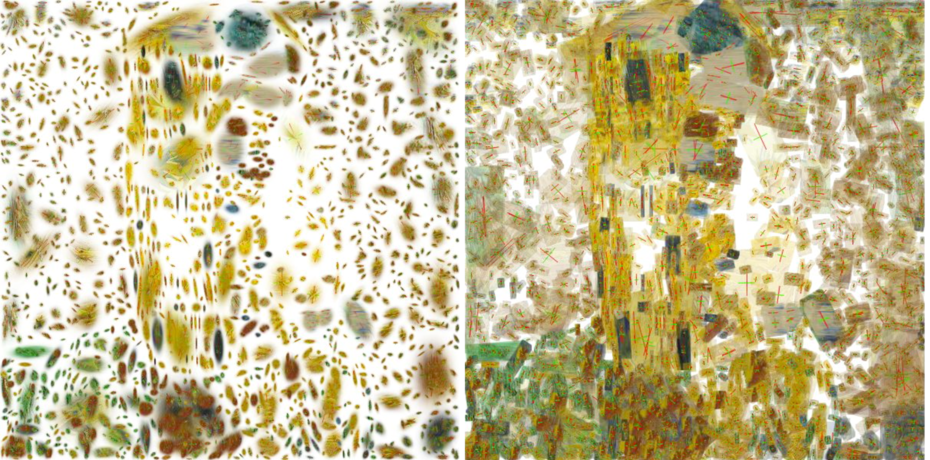
\includegraphics[width=3.1in]{images/spatial-blending-3.png}
  
  \caption{Using the target image and database shown in Figure-\ref{fig:teaser}, we show an example stylization with (first image) and without (second image) spatial blending.  We also draw the region's orientation depicted by red/green axes in order to better show the regions (best viewed in the color manuscript at 200\%).}
  \label{fig:spatial-blending}
\end{figure}
\begin{figure}[ht]
  \centering
  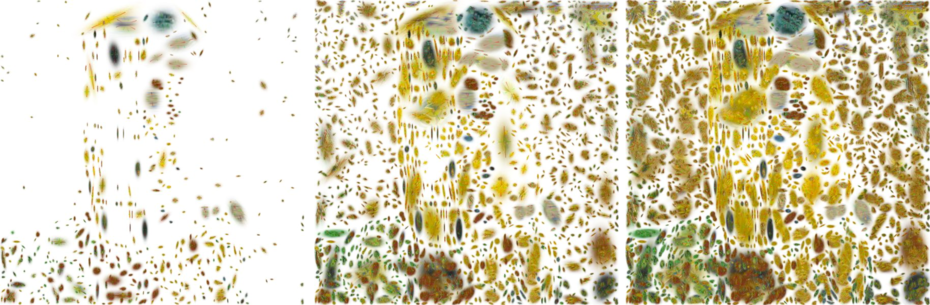
\includegraphics[width=3.1in]{images/increasing-timesteps-2.png}
  
  \caption{Using the target image and database shown in Figure-\ref{fig:teaser}, the timesteps are increased over time.  This allows the user to detect more regions and develop a denser and higher contrast stylization.}
  \label{fig:timesteps}
\end{figure}
\begin{figure}[ht]
  \centering
  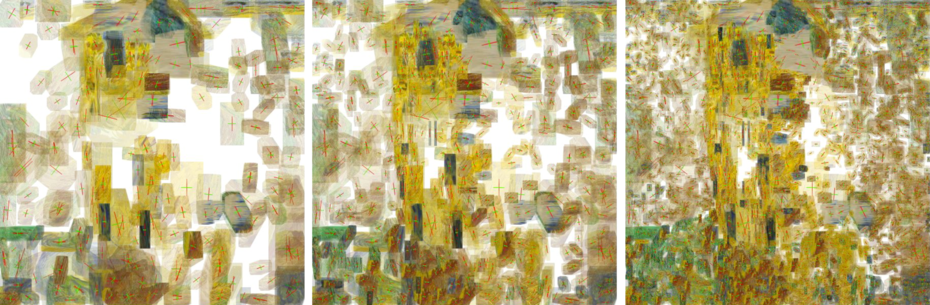
\includegraphics[width=3.1in]{images/decreasing-minimum-size-2.png}
  
  \caption{Using the target image and database shown in Figure-\ref{fig:teaser}, the minimum region size is decreased over time, allowing the user to detect smaller regions and produce finer detailed stylizations.}
  \label{fig:minimum-size}
\end{figure}
\begin{figure}[ht]
  \centering
  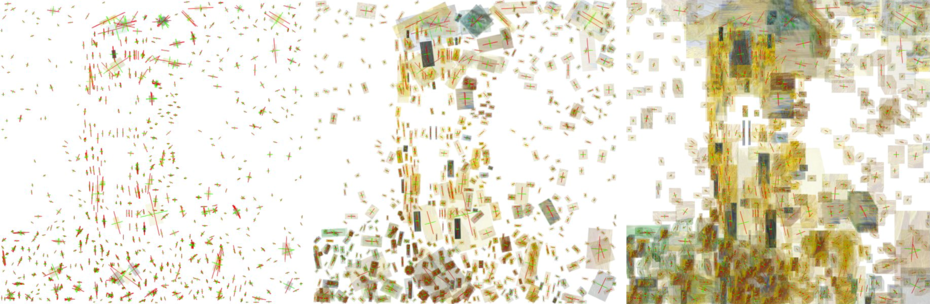
\includegraphics[width=3.1in]{images/blending-radius-2.png}
  
  \caption{Using the target image and database shown in Figure-\ref{fig:teaser}, the blending radius is increased over time.  This parameter influences the overall size of the drawn regions.  Setting this number smaller can help to produce finer details on top of existing layers, often associated with both Impressionist and Abstract Expressionist styles.}
  \label{fig:blending-radius}
\end{figure}
\begin{figure}[ht]
  \centering
  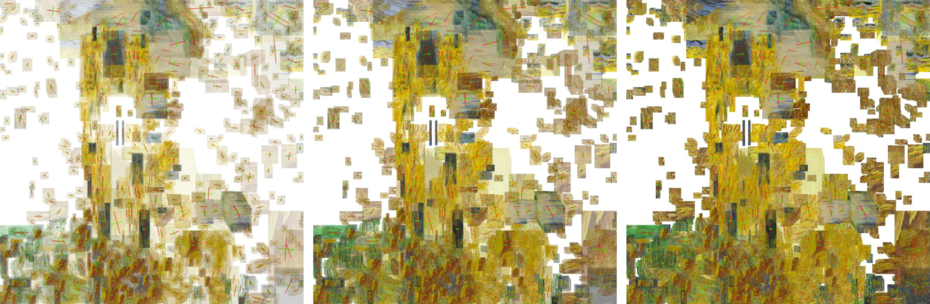
\includegraphics[width=3.1in]{images/temporal-blending.png}
  
  \caption{Using the target image and database shown in Figure-\ref{fig:teaser}, we increase the temporal blending factor.  This influences the opacity of every region drawn. }
  \label{fig:temporal-blending}
\end{figure}
\begin{figure}[ht]
  \centering
  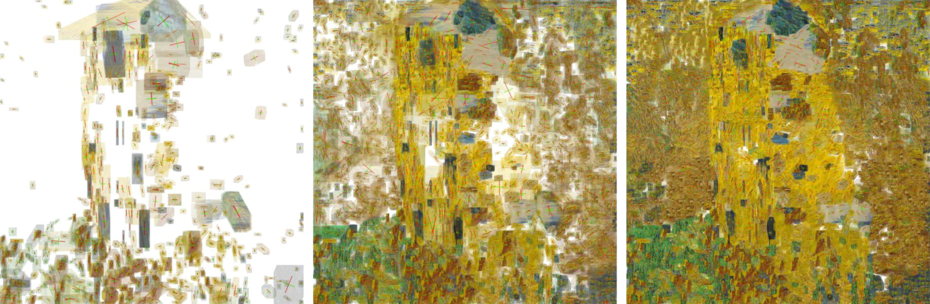
\includegraphics[width=3.1in]{images/temporal-blending-changing-params.png}
  
  \caption{Using the target image and database shown in Figure-\ref{fig:teaser}, we use temporal blending as well as decreasing minimum region size and increased timesteps to begin to produce the final synthesis.}
  \label{fig:temporal-blending-changing-parameters}
\end{figure}
For the target, we allow the user to interactively define a few parameters affecting the output stylization.  
\begin{itemize}
\item \textit{Spatial blending}: Allows the user to use feathered elliptical regions instead of rectangular ones (see Figure-\ref{fig:spatial-blending}).  When stylizing finer details of an image, this parameter is very useful for removing hard edges produced by rectangular regions.  
\item \textit{Timesteps}: Increasing this produces more regions, making the image denser (see Figure-\ref{fig:timesteps}).  As well, this will also produce more regions that coincide with each other.  As a result, when synthesizing with a high number for the timesteps, the result resembles an overpainting effect.  For styles that require many ``layers'' of ``paint'', we use a higher number for the timesteps.  When used in combination with blending, increasing this can also increase the contrast.
\item \textit{Minimum region size}: This parameter determines the minimum allowed region size for synthesis.  Setting this number very low (e.g. below 100 pixels) produces styles more similar to Impressionism, as many small regions are detected (see Figure-\ref{fig:minimum-size}).  
\item \textit{Maximum region size}: Similar to the minimum region size parameter, this parameter determines the largest allowed region size. Generally setting this number as high as possible will be sufficient.  However, it may be desirable to interactively change this parameter over time, allowing for large regions to be drawn at first, then only allowing smaller ones. 
\item \textit{Temporal blending}: Uses alpha blending to composite regions over time (see Figure-\ref{fig:temporal-blending}).  Together with an increased number of timesteps, this parameter can be used to change the contrast of the overall image (as shown in Figure-\ref{fig:temporal-blending-changing-parameters}).  
\item \textit{Motion tracking}: Allows regions to be drawn only if their detected motion is higher than a fixed threshold.  For our experiments, we set this number to 5.  
\item \textit{Blending radius}: Influences the feathering radius of the detected region (see Figure-\ref{fig:blending-radius}).  Normally, each detected region is matched to one in the database and then through an affine transformation placed where the detected region was using the same scale and rotation.  However, it may be desirable to change the scale of this region using the blending radius to produce different effects.  When scaling this region down, a user confines drawing to only small regions being painted, often produces styles associated with Abstract Expressionism.
\end{itemize}
For image-based targets, the aforementioned parameters effect the frame-to-frame compositing, meaning the same image is rendered over itself.  For video-based targets, however, only a single iteration is used for each frame, as much of the information required for building styles requiring more detailed composites can be extracted over the first 1 or 2 frames.  We demonstrate how these parameters can influence a wide range of stylizations in the next section.
\section{Results}  
\label{sec:results}
We use the presented framework to produce artistic stylizations of photo-realistic images and videos.  In this section, we show our results in image-based stylization using a landscape, abstract, and painterly scene. We then show how the same framework can be used with video targets, including an abstract and portrait video.  As well, we show a particular case where the source material is aggregated from a live-stream of the target, i.e. the source and target are the same, a process we call ``Memory Mosaicing''.  

\subsection{Image: Landscape}\vspace{-0.4em}
\begin{figure*}[ht]
  \centering
  \includegraphics[width=\textwidth]{images/cows-klee.png}
  \caption{A landscape picture of cows grazing is synthesized using 13 images of Expressionism painter Paul Klee to produce the image on the right.  Images representing faithful reproductions of Paul Klee sourced from \href{http://www.artchive.com/}{Mark Harden's Artchive} are public domain. Photo of cows taken by the author.}
  %www.sai.msu.su/wm/paint/auth/klee/
  %This work is in the public domain in the United States because it was first published outside the United States (and not published in the U.S. within 30 days) and it was first published before 1978 without complying with U.S. copyright formalities or after 1978 without copyright notice and it was in the public domain in its home country on the URAA date (January 1, 1996 for most countries).
  %This work is in the public domain in the European Union and non-EU countries with a copyright term of life of the author plus 70 years or less.
  \label{fig:cows-klee}
\end{figure*}
In Figure-\ref{fig:cows-klee}, we synthesize a landscape photo of cows grazing using Expressionist painter Paul Klee.  We turn off spatial blending and use a small value for the minimum region size.  We also allow the maximum region size to be very large.  This results in a relatively smaller region being matched to the sky and stretched to fill the top-half of the image.  The synthesized region happens to look like a rainbow, though the original region itself was very abstract (see the first image in the second row of the Klee corpus).  
\subsection{Image: Abstract}\vspace{-0.4em}
\begin{figure*}[ht]
  \centering
  \includegraphics[width=\textwidth]{images/blanket-klimt.png}
  \caption{A close-up picture of a blanket is synthesized using Klimt's The Kiss to produce the image on the right. Best viewed in the color manuscript at 200\%. Images representing faithful reproductions of Gustav Klimt sourced from \href{http://commons.wikimedia.org}{Wikimedia Commons} are public domain.  Photorealistic scene of blanket taken by the author.}
  %https://en.wikipedia.org/wiki/File:Gustav_Klimt_016.jpg
  \label{fig:blanket-klimt}
\end{figure*}
In Figure-\ref{fig:blanket-klimt}, we synthesize a close-up picture of a blanket using Klimt's The Kiss.  The target this time is very abstract and we will not need to synthesize parameters that force an abstract quality rendering such as large region sizes.  As such, we allow the minimum region size to be very small producing more details, though retaining a style associated with Abstract Expressionism.
\subsection{Image: Painterly}\vspace{-0.4em}
\begin{figure*}[ht]
  \centering
  \includegraphics[width=\textwidth]{images/van-gogh-monet.png}
  \caption{Van Gogh's ``The Bedroom'' is synthesized using 3 images of Monet paintings to produce the image on the right. Images representing faithful reproductions of Van Gogh and Claude Monet sourced from \href{http://commons.wikimedia.org}{Wikimedia Commons} are public domain.}
  %https://commons.wikimedia.org/wiki/File:La_Chambre_%C3%A0_Arles,_by_Vincent_van_Gogh,_from_C2RMF.jpg
  %https://en.wikipedia.org/wiki/File:Claude_Monet,_Impression,_soleil_levant,_1872.jpg
  %https://en.wikipedia.org/wiki/File:Bridge_Over_a_Pond_of_Water_Lilies,_Claude_Monet_1899.jpg
  %https://en.wikipedia.org/wiki/File:Monet_Water_Lilies_1916.jpg
  \label{fig:van-gogh-monet}
\end{figure*}
We demonstrate how CBVS can stylize existing painterly images into other styles.  In the teaser graphic in Figure-\ref{fig:teaser}, we use three paintings by Van Gogh to stylize Klimt's The Kiss.  Here, we set the minimum region size to be small, allowing finer details and smaller brush strokes, and allow the timesteps to be high as we want to bring out as much contrast as possible.  

In Figure-\ref{fig:van-gogh-monet}, we try synthesizing Van Gogh's The Bedroom using 3 images of Monet's Water Lilies series.  Here, we ensure we detect many small regions by increasing the timesteps and setting the minimum region size to be very small.  Further, we turn on spatial blending as we decrease the minimum region size, as we want to avoid rendering any strong edges, retaining an Impressionist quality.
\subsection{Video: Portrait}
\begin{figure}[ht]
  \centering
  \includegraphics[width=2.8in]{images/dad-rowing-4x2.png}
  \caption{Left: 4 frames from a target video; Right: Stylization using Paul Klee's corpus in Figure-\ref{fig:cows-klee}.  We aim to synthesize with greater expression and less abstraction, and allow the minimum region size to be very small. Best viewed in the color manuscript at 200\% or in the video online. Photos by the author.}
  \label{fig:rowing}
\end{figure}
Two examples in video-based stylization are presented: one of a subject rowing a boat and another of abstract imagery.  In Figure-\ref{fig:rowing}, we can see 4 frames taken from a video stylization.  We use the same corpus as in Figure-\ref{fig:cows-klee} and allow the minimum region size to be very small, resulting in a more Expressionist style.  The first frame is not as composed as the later frames, as there will have only been 1 frame of compositing.  As a result, the first frame in video-based Expressionist stylization may not be a consistent style with its later frames.
\subsection{Video: Abstract}\vspace{-0.4em}
\begin{figure}[ht]
  \centering
  \includegraphics[width=2.8in]{images/blanket-video.png}
  \caption{Left: 4 frames from a target video; Right: Stylization using Paul Klee's corpus in Figure-\ref{fig:cows-klee}.  Here we aim to stylize with greater abstraction than in Figure-\ref{fig:rowing}, and set the minimum region size to be fairly large. Best viewed in the color manuscript at 200\% or in the video online.   Photos by the author.}
  \label{fig:blanket-video}
\end{figure}
In Figure-\ref{fig:blanket-video}, we stylize a video using the same corpus as in Figure-\ref{fig:cows-klee} and set the minimum region size to be very large.  Thus, instead of producing an Expressionist style as in Figure-\ref{fig:rowing}, less details are synthesized resulting in a more abstract style.  The first frame in this video does not necessarily require more than 1 iteration as it is synthesizing very large regions that often also overlap.

\subsubsection{Video: The Simpsons vs. Family Guy}

70k views and Vimeo Staff Pick, and selected for exhibition twice, once at the Tin Shed Gallery in London, UK, and again at the Media Art Histories conference during the ART+COMMUNICATION: SAVE AS Exhibition in Riga, Latvia.

\subsection{Memory Mosaicing}\vspace{-0.4em}
% picture of memory mosaicing as video thumbnails

The artistic stylization process can be used in a real-time context without an explicit corpus.  In this case, we aggregate representations learned from the ongoing stream of target frames.  Parameters are generally set by the user interacting with the process, or contained to a single preset.  In particular, restricting the total number of representations as first-in-first-out queue allows the process to continue in real-time with a simple linear search index.  In the examples shown in Figure \ref{fig:memory-mosaicing}, we show two example outputs from the same camera stream.  In the left image, we aim for large region sizes and low timesteps, resulting in a more abstract style, reminiscent of Cubist style paintings.  In the right example, we allow higher timesteps and only small region sizes, resulting in a more expressive style similar to paintings in Abstract Expressionism.  

\section{Discussion and Future Works}
We have presented a framework for producing artistic stylizations of images or videos.  A corpus of image material is automatically segmented, defining the possible strokes effecting the possible colors and textures in the stylization.  Using a simple set of parameters, we have shown that many stylizations of a target image or video are possible, ranging from Impressionism, Expressionism, and Abstract Expressionism.  By allowing the interactive refinement of an image's stylization, we allow the user to experiment with a range of stylizations through simple parameters.  This interactive refinement affords compositing, the ability to blend together stylizations from different parameters over time.  We also demonstrate the extension of this framework to video-based stylization using simple motion tracking.  As in image-based stylization, the user can influence the stylization through the same set of parameters in real-time to interactively refine the stylization.  

The extension of video-based stylization is also particularly suited for real-time contexts as shown in ``Memory Mosaicing'', where a database is aggregated from learning representations in a target frame over time. 

A number of issues could be addressed in future versions.  For instance, synthesized regions with poor shape matches can be heavily distorted in a resulting synthesis.  In these cases, it is likely that the database did not include any other matches with more similar shapes, or the shape descriptor had been weighted too low.  As well, the speed of the synthesis in a real-time context can be greatly improved with other search methods such as tree or hash-table based indexes.  As well, our approach to addressing the temporal coherence of the resulting stylization may be improved with investigating incorporating more recent models of optical flow, keyframe detection, and possibly spatiotemporal detection of representations rather than purely spatial ones.   
%\section*{Acknowledgements}
%Thanks to Baptiste Caramiaux and Atau Tanaka for their comments on an earlier draft.  Also thanks to Enrica Cassentini for her help in creating a children's painting and earlier tests in stylization.  
%%% Please use the ``acmsiggraph'' BibTeX style to properly format your
%%% bibliography.

\begin{figure}[h]
  \centering
  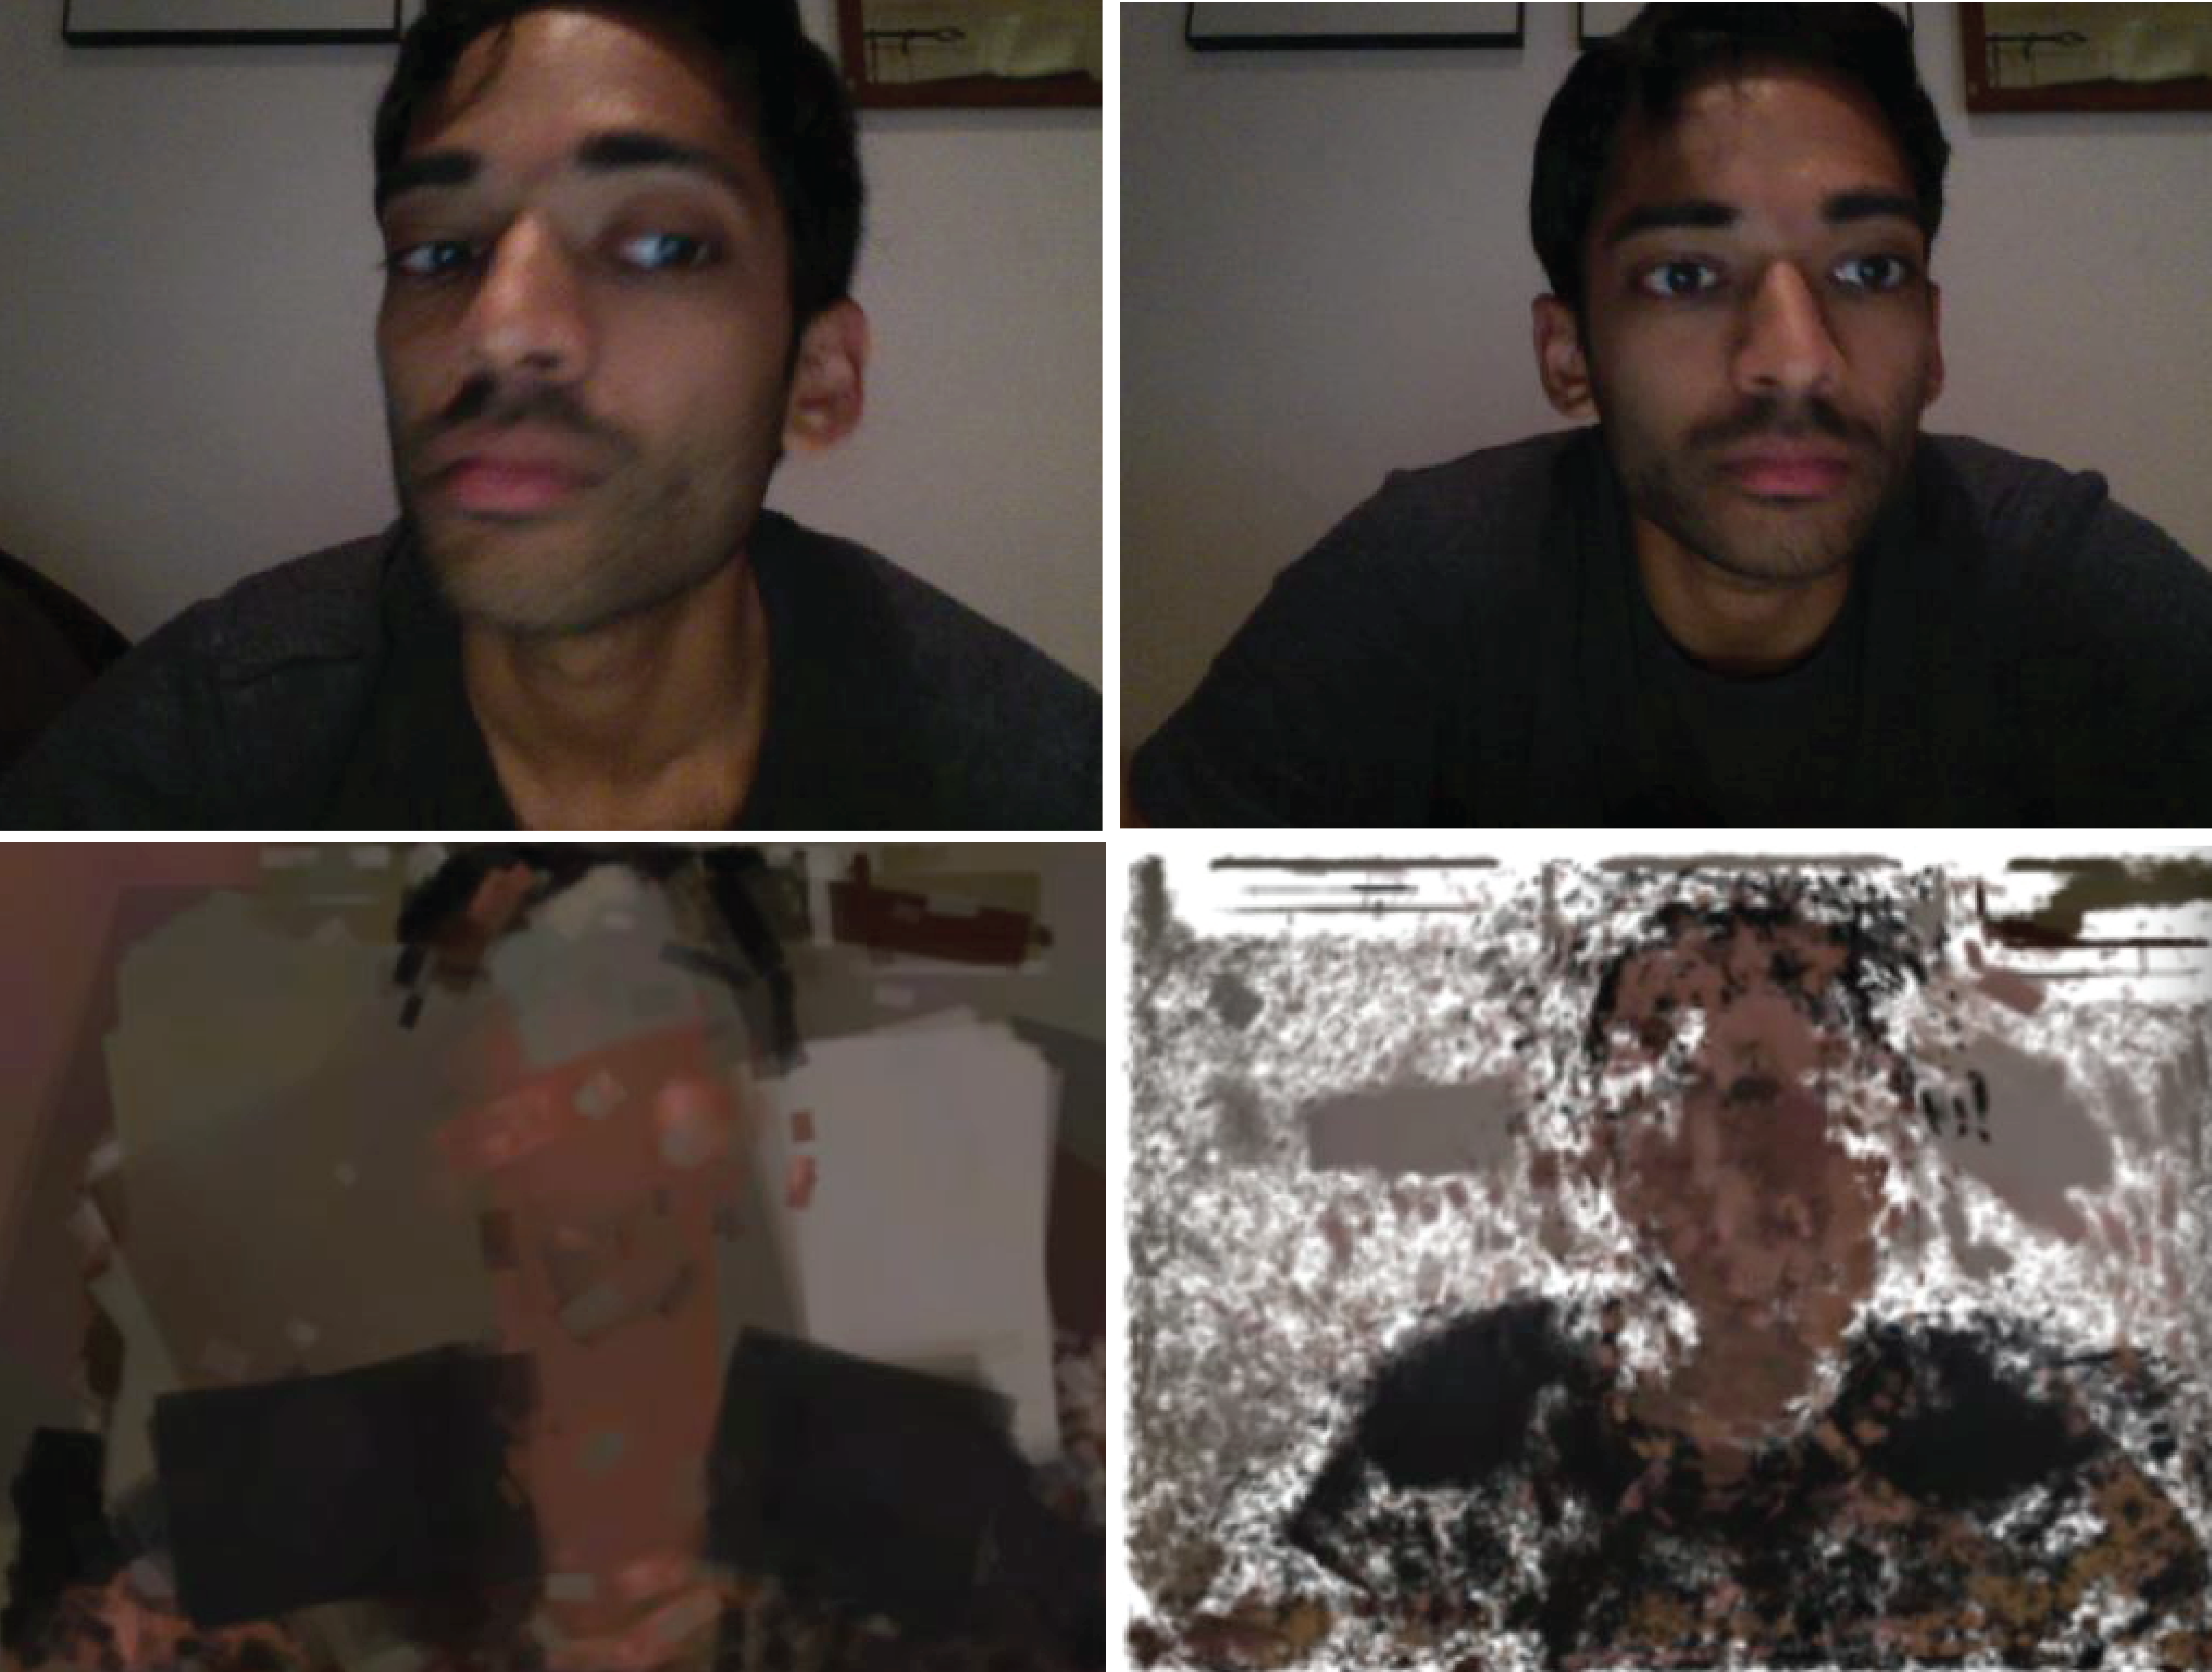
\includegraphics[width=2.8in]{images/memory-mosaic-2x2.png}
  \caption{2 examples of ``Memory Mosaicing'' showing the input (top) and resulting real-time stylization (bottom).   Photos by the author.}
  \label{fig:memory-mosaicing}
\end{figure}



%%%%%%%%%%%%%%%%%%%%%%%%%%%%%%%%%%%%%%%%%%%%%%%%%%%
%%%%%%%%%%%%%%%%%%%%%%%%%%%%%%%%%%%%%%%%%%%%%%%%%%%
%%%%%%%%%%%%%%%%%%%%%%%%%%%%%%%%%%%%%%%%%%%%%%%%%%%
%%%%%%%%%%%%%%%%%%%%%%%%%%%%%%%%%%%%%%%%%%%%%%%%%%%
%%%%%%%%%%%%%%%%%%%%%%%%%%%%%%%%%%%%%%%%%%%%%%%%%%%
%%%%%%%%%%%%%%%%%%%%%%%%%%%%%%%%%%%%%%%%%%%%%%%%%%%
%%%%%%%%%%%%%%%%%%%%%%%%%%%%%%%%%%%%%%%%%%%%%%%%%%%



%%%%%%%%%%%%%%%%%%%%%%%%%%%%%%%%%%%%%%%%%%%%%%%%%%%
%%%%%%%%%%%%%%%%%%%%%%%%%%%%%%%%%%%%%%%%%%%%%%%%%%%
%%%%%%%%%%%%%%%%%%%%%%%%%%%%%%%%%%%%%%%%%%%%%%%%%%%
%%%%%%%%%%%%%%%%%%%%%%%%%%%%%%%%%%%%%%%%%%%%%%%%%%%
%%%%%%%%%%%%%%%%%%%%%%%%%%%%%%%%%%%%%%%%%%%%%%%%%%%
%%%%%%%%%%%%%%%%%%%%%%%%%%%%%%%%%%%%%%%%%%%%%%%%%%%
%%%%%%%%%%%%%%%%%%%%%%%%%%%%%%%%%%%%%%%%%%%%%%%%%%%

\chapter{Computational Audiovisual Scene Synthesis}
\label{ch:audiovisual}
\minitoc

\section{Introduction}

Talk about attempts to combine models in perception and practice.   DIEM model, how do you combine two modalities.

Classic effects in crossmodal/multisensory perception

Unresolved scientific questions... hence parallel...

\section{Augmented Reality Hallucination}

\begin{figure}
  \centering
  \includegraphics[width=2.4in]{images/vam.png}
  \caption{An exhibition at the Victoria and Albert Museum in London had participants wear Augmented Reality goggles with software running a real-time version of ``Memory Mosaicing''.  Photos by the author.}
  \label{fig:vam}
\end{figure}
\begin{figure}
  \centering
  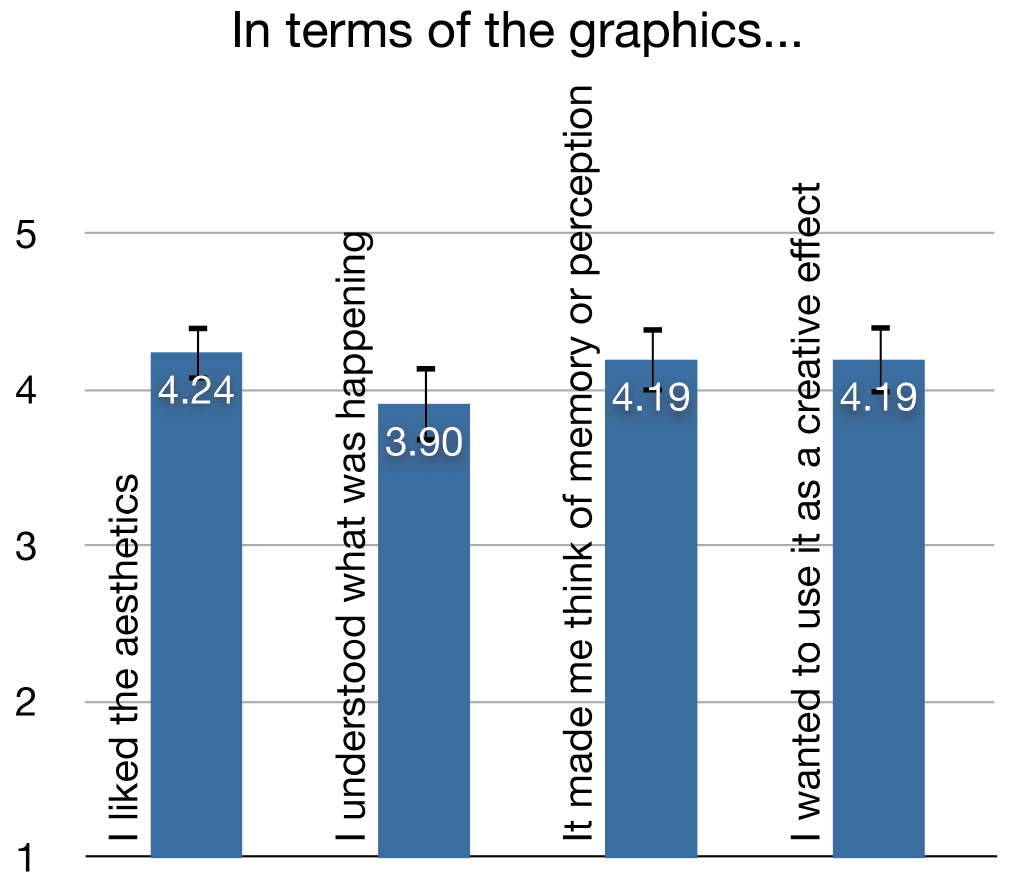
\includegraphics[width=2.4in]{images/vam-graphics-bar-resize-01.png}
  \caption{Results of the ``Augmented Reality Hallucination'' installation feedback where 21 participants were asked to rate different aspects of the visual synthesis.  Error bars depict +/- 1 S.E.}
  \label{fig:vam-graphics-bar}
\end{figure}

An interesting case of ``Memory Mosaicing'' is when a participant can actively explore a visual scene.  By using augmented reality goggles, we allowed participants to explore their environment through the our proposed stylization process during an exhibition called ``Augmented Reality Hallucinations'' held at the Victoria and Albert Museum in London.  Participants were invited to wear the goggles where two small CRT screens presented the same output of a ``Memory Mosaicing'' of a single camera mounted on the goggles right eye that faced the scene in front of them (see Figure \ref{fig:vam}).  As the only user interaction was in exploring a scene, a single preset was defined based on large region sizes and low number of timesteps.  

Participants were also invited to give quantitative and qualitative feedback on their experience.  The summary of the quantitative feedback is shown in Figure \ref{fig:vam-graphics-bar}.  On the feedback form, when participants were asked, ``Did this experience make you think of anything you had seen or heard before?'', three participants made references to their experiences on hallucinogens and two to dreams.  Also of note in the qualitative feedback was references to art styles such as, ``It reminded me of Francis Bacon's Figurative style'' and ``The movement was Impressionistic, almost painterly''.  When asked, ``What did you dislike most about the experience?'', of note were the responses, ``Would have liked more depth in colour'', ``Not sure what I was seeing at first with the goggles'', and ``Hard to understand how it works.''  The lack of understanding of the process may also be revealed in the quantitative analysis in the second bar of the graph.  However, on average, this number is still quite high across participants, though there is also no baseline to compare to.  

\subsection{Hardware}
\subsubsection{Vuzix Wrap20AR}
\subsubsection{Oculus Rift}


\section{YouTube Smash Up}



\subsection{YouTube Content ID}

In October 2007, YouTube introduced a content management tool, Video ID, to help content owners find infringing material.  Block, track, monetize.

Margaret Gould Stewart, YouTube's head of content revealed in a TED talk \cite{Stewart2010},

\begin{quotationb}
Here we can see the reference file being compared to the user generated content. The system compares every moment of one to the other to see if there's a match. This means we can identify a match even if the copy uses just a portion of the original file, plays it in slow motion, and has degraded audio or video.  The scale and speed of this system is truly breathtaking -- we're not just talking about a few videos, we're talking about over 100 years of video every day between new uploads and the legacy scans we regularly do across all of the content on the site. And when we compare those 100 years of video, we're comparing it against millions of reference files in our database. It'd be like 36,000 people staring at 36,000 monitors each and every day without as much as a coffee break.
\end{quotationb}

Smitelli's reverse engineering of YouTube's Content ID system revealed a number of parameters which could and could not be detected by their system \cite{Smitelli2009}.  

Though one month after the 2012 fall democratic convention speech featuring first lady Michelle Obama was aired and subsequently taken down due to copyright infringement \cite{Singel2012}, YouTube released a statement saying they would enforce manual reviewing of more of their copyright claims by the content owners in an effort to reduce erroneous claims \cite{Alfishawi2012}.  


%%%%%%%%%%%%%%%%%%%%%%%%%%%%%%%%%%%%%%%%%%%%%%%%%%%
%%%%%%%%%%%%%%%%%%%%%%%%%%%%%%%%%%%%%%%%%%%%%%%%%%%
%%%%%%%%%%%%%%%%%%%%%%%%%%%%%%%%%%%%%%%%%%%%%%%%%%%
%%%%%%%%%%%%%%%%%%%%%%%%%%%%%%%%%%%%%%%%%%%%%%%%%%%
%%%%%%%%%%%%%%%%%%%%%%%%%%%%%%%%%%%%%%%%%%%%%%%%%%%
%%%%%%%%%%%%%%%%%%%%%%%%%%%%%%%%%%%%%%%%%%%%%%%%%%%
%%%%%%%%%%%%%%%%%%%%%%%%%%%%%%%%%%%%%%%%%%%%%%%%%%%



%%%%%%%%%%%%%%%%%%%%%%%%%%%%%%%%%%%%%%%%%%%%%%%%%%%
%%%%%%%%%%%%%%%%%%%%%%%%%%%%%%%%%%%%%%%%%%%%%%%%%%%
%%%%%%%%%%%%%%%%%%%%%%%%%%%%%%%%%%%%%%%%%%%%%%%%%%%
%%%%%%%%%%%%%%%%%%%%%%%%%%%%%%%%%%%%%%%%%%%%%%%%%%%
%%%%%%%%%%%%%%%%%%%%%%%%%%%%%%%%%%%%%%%%%%%%%%%%%%%
%%%%%%%%%%%%%%%%%%%%%%%%%%%%%%%%%%%%%%%%%%%%%%%%%%%
%%%%%%%%%%%%%%%%%%%%%%%%%%%%%%%%%%%%%%%%%%%%%%%%%%%

\chapter{Conclusion}
\label{ch:conclusion}
\minitoc

\section{Summary}
\section{Contribution}
\section{Limitations}
\section{Future Work}
\section{Final Discussion}




%%%%%%%%%%%%%%%%%%%%%%%%%%%%%%%%%%%%%%%%%%%%%%%%%%%
%%%%%%%%%%%%%%%%%%%%%%%%%%%%%%%%%%%%%%%%%%%%%%%%%%%
%%%%%%%%%%%%%%%%%%%%%%%%%%%%%%%%%%%%%%%%%%%%%%%%%%%
%%%%%%%%%%%%%%%%%%%%%%%%%%%%%%%%%%%%%%%%%%%%%%%%%%%
%%%%%%%%%%%%%%%%%%%%%%%%%%%%%%%%%%%%%%%%%%%%%%%%%%%
%%%%%%%%%%%%%%%%%%%%%%%%%%%%%%%%%%%%%%%%%%%%%%%%%%%
%%%%%%%%%%%%%%%%%%%%%%%%%%%%%%%%%%%%%%%%%%%%%%%%%%%



%%%%%%%%%%%%%%%%%%%%%%%%%%%%%%%%%%%%%%%%%%%%%%%%%%%
%%%%%%%%%%%%%%%%%%%%%%%%%%%%%%%%%%%%%%%%%%%%%%%%%%%
%%%%%%%%%%%%%%%%%%%%%%%%%%%%%%%%%%%%%%%%%%%%%%%%%%%
%%%%%%%%%%%%%%%%%%%%%%%%%%%%%%%%%%%%%%%%%%%%%%%%%%%
%%%%%%%%%%%%%%%%%%%%%%%%%%%%%%%%%%%%%%%%%%%%%%%%%%%
%%%%%%%%%%%%%%%%%%%%%%%%%%%%%%%%%%%%%%%%%%%%%%%%%%%
%%%%%%%%%%%%%%%%%%%%%%%%%%%%%%%%%%%%%%%%%%%%%%%%%%%

\appendix
\chapter{Appendix}
\label{chap:appendix1}
\bibliographystyle{ThesisStyle}
\bibliography{library}
%\printnomenclature
\end{document}
